% !TEX root = ln_diss.tex
\graphicspath{{img/ch1/}}
\chapter{Finite elements for the wave equation} \label{chap:FE}

\par This chapter introduces the boundary value problem that describes the radiation mechanism in an unbounded medium. The vector wave equation is then derived from Maxwell's eqations, being the partial differential equation that describes waves propagation. The finite element formulation for the electric field wave equation follows, presented for a full-wave solution of electromagnetic radiation problems. Several boundary conditions, that will be used throughout this dissertation, will be introduced here, allowing for the treatment of fields propagation analysis from either waveguides ports or free-space impinging waves. Some test cases will be shown, comparing to a commercial package, analyzing the FES implemented formulations behavior. FES is the core of the domain decomposition and the nonlinear analyzes presented, respectively, in chapters \ref{chap:DD} and \ref{chap:NL}.

%%%%%%%%%%%%%%%%%%%%%%

\section{Radiation in an unbounded medium}

\par The problem of electromagnetic radiation from a generic distribution of current sources in a unbounded medium relies on the solution of the Maxwell's equations \cite{rothwell2009electromagnetics}
\begin{eqnarray}
\nabla \times \mathcalb{E}(\mathbf{r},t) &= & -\frac{\partial}{\partial t}\mathcalb{B}(\mathbf{r},t) \qquad \qquad \qquad \quad \mathit{Faraday}\textrm{'}\mathit{\!s \ law}, \label{eq:tfaraday}  \\
\nabla \times \mathcalb{H}(\mathbf{r},t) &= & \frac{\partial}{\partial t}\mathcalb{D}(\mathbf{r},t) + \mathcalb{J}(\mathbf{r},t)  \quad \ \ \textit{Maxwell-Amp\`{e}re}\textrm{'}\mathit{\!s \ law}, \label{eq:tampere} \\[5pt]
\nabla \cdot \mathcalb{D}(\mathbf{r},t) &= & {\varrho}(\mathbf{r},t) \qquad \qquad \qquad \qquad \  \mathit{Poisson}\textrm{'}\mathit{\!s \ equation}, \label{eq:tpoisson}\\[5pt]
\nabla \cdot \mathcalb{B}(\mathbf{r},t) &= & 0 \qquad \qquad \qquad \qquad 	\ \ \ \ \mathit{Gauss}\textrm{'}\mathit{\! \ law \ for \ magnetism}, \label{eq:tgauss}
\end{eqnarray} where $\mathcalb{E}$ is the \textit{electric field intensity}, which carries the S.I.\footnote{Syst\`eme International d'unit\'es.} units $\mathrm{\nicefrac{\mathrm V}{\mathrm m}}$, $\mathcalb{H}$ the \textit{magnetic field intensity} in $\mathrm{\nicefrac{\mathrm A}{\mathrm m}}$, $\mathcalb{D}$ the \textit{electric displacement} in $\mathrm{\nicefrac{\mathrm C}{m^2}}$ (or $\mathrm{\nicefrac{\mathrm{As}}{m^3}}$), $\mathcalb{B}$ the \textit{magnetic induction} in $\mathrm{\nicefrac{\mathrm{Wb}}{m^2}}$ (or $\mathrm{\nicefrac{\mathrm{Vs}}{m^2}}$), $\mathcalb{J}$ the \textit{electric current density} in $\mathrm{\nicefrac{\mathrm A}{\mathrm m}}$ and $\mathcal{\varrho}$ the \textit{electric charge density} in $\mathrm{\nicefrac{\mathrm C}{m^3}}$ (or $\mathrm{\nicefrac{\mathrm{As}}{m^3}}$).
 All these values are dependent on the position vector $\mathbf{r} \in \mathbb{R}^3$ and on the time variable $t \in \mathbb{R}$. Combining the divergence of \eqref{eq:tampere} with \eqref{eq:tpoisson}, we obtain the \textit{current continuity equation}
\begin{equation}
\nabla \cdot \mathcalb{J}(\mathbf{r},t) + \frac{\partial}{\partial t} \mathcal{\varrho}(\mathbf{r},t) = 0.
\end{equation}
\par In order to solve Maxwell's system of first order partial differential equations (PDEs), it is necessary to provide the \textit{boundary conditions} and the \textit{initial conditions}. Furthermore, as the number of equations is less than the number of unknowns, we need to supply the \textit{constitutive relations}, which relates the electric displacement and the magnetic induction to the fields
\begin{eqnarray}
\label{eq:constgen1}
\mathcalb{D}(\mathbf{r},t) &= & \dyad{\epsilon}(\mathbf{r},t) \cdot \mathcalb{E}(\mathbf{r},t) \\
\label{eq:constgen2}
\mathcalb{B}(\mathbf{r},t) &= &  \dyad{\mu}(\mathbf{r},t) \cdot \mathcalb{H}(\mathbf{r},t),
\end{eqnarray} 
where $\dyad{\epsilon}$ and $\dyad{\mu}$ are dyadic tensors depending on the material in which the fields exist\footnote{The constitutive relations in (\ref{eq:constgen1}-\ref{eq:constgen2}) are stated in a form such that they can represent \textit{isotropic} and \textit{anisotropic} media.}. Also, in presence of conductive materials, the electric field gives birth to an electric current density
\begin{eqnarray}
\mathcalb{J}^c(\mathbf{r},t) &= &\dyad{\sigma}(\mathbf{r},t) \cdot \mathcalb{E}(\mathbf{r},t) \qquad \mathit{Ohm}\textrm{'}\mathit{\!s \ law},
\end{eqnarray}
where $\dyad{\sigma}$ is the \textit{electric conductivity} dyadic tensor in $\mathrm{\nicefrac{\mathrm S}{\mathrm m}}$, and the superscript \textit{c} on $\mathcalb{J}^c(\mathbf{r},t)$ indicates that the current density is induced by the electric field. With this additional equation, the current $\mathcalb{J}(\mathbf{r},t)$ in \eqref{eq:tampere} can be considered to be composed by an induced part, $\mathcalb{J}^c(\mathbf{r},t)$, and by an impressed part, $\mathcalb{J}^i(\mathbf{r},t)$, the latter actually being the source generating the electromagnetic fields.
%For a unbounded medium, the boundary conditions are those that ensure the fields extinction out of the domain investigated. This is possible by forcing the 
\par The boundary conditions ensure the continuity of the fields at the interfaces between different media, and this is stated as\footnote{The continuity equations (\ref{eq:conte1}-\ref{eq:contb1}) are derived from an integral solution of the Maxwell's equations, assuming a connected volume made by a part of region 1 and a part of region 2, i.e. a closed surface crossing the boundary interface between the two regions.}, for a surface interfacing two media,
\begin{eqnarray}
\hat{\mathbf{n}} \times \left ( \mathcalb{E}_1(\mathbf{r},t)-\mathcalb{E}_2(\mathbf{r},t) \right ) &= & 0,  \label{eq:conte1} \\
\hat{\mathbf{n}} \times \left ( \mathcalb{H}_1(\mathbf{r},t)-\mathcalb{H}_2(\mathbf{r},t) \right ) &= & \mathcalb{J}_s(\mathbf{r},t), \\
\hat{\mathbf{n}} \cdot \left ( \mathcalb{D}_1(\mathbf{r},t)-\mathcalb{D}_2(\mathbf{r},t) \right ) &= & \varrho_s(\mathbf{r},t), \\
\hat{\mathbf{n}} \cdot \left ( \mathcalb{B}_1(\mathbf{r},t)-\mathcalb{B}_2(\mathbf{r},t) \right ) &= & 0, \label{eq:contb1}
\end{eqnarray}
where $\hat{\mathbf{n}}$ is the unit vector normal to the surface, outwardly directed from the first region. $\mathcalb{J}_s$ and $\rho_s$ are the \textit{electric surface current density} in $\mathrm{\nicefrac{\mathrm A}{\mathrm m}}$ and \textit{electric surface charge density} in $\mathrm{\nicefrac{\mathrm C}{m^2}}$. %By (\ref{eq:conte1}-\ref{eq:contb1}), we obtain surface current and charge densities that keep informations on the fields outside (region 2) of the region in which the Maxwell's equations are solved (region 1), as if the whole domain were ununbounded.

\par For the radiation problem we need to solve in this chapter, we will consider \textit{isotropic} (\textit{homogeneous}) and \textit{time-invariant} media, for which the dyadics relating the fields to the electric displacement and magnetic induction are scalar values (diagonal tensors with equal entries). Thus, the constitutive relations become
\begin{eqnarray} 
\mathcalb{D}(\mathbf{r},t) &= \ \ \ \epsilon \mathcalb{E}(\mathbf{r},t) &= \ \ \ \epsilon_0 \epsilon_r \mathcalb{E}(\mathbf{r},t),  \label{eq:fsconst1}\\
\mathcalb{B}(\mathbf{r},t) &= \ \ \ \mu \mathcalb{H}(\mathbf{r},t)  &= \ \ \ \mu_0 \mu_r \mathcalb{H}(\mathbf{r},t), \label{eq:fsconst2}
\end{eqnarray}
where the constant $\epsilon_0 = 8.854 \times 10^{-12} \ \mathrm{\nicefrac{\mathrm F}{\mathrm m}}$ is the \textit{free-space permittivity}, $\epsilon_r$ the \textit{relative permittivity}, a non-dimensional constant, $\mu_0 = 4\pi \times 10^{-7} \ \mathrm{\nicefrac{\mathrm H}{\mathrm m}}$ is the \textit{free-space permeability} and $\mu_r$ the \textit{relative permeability}, also non-dimensional. As we expect electromagnetic waves to be propagating, we denote their speed as  $c = \nicefrac{1}{\sqrt{\epsilon \mu}} = \nicefrac{c_0}{\sqrt{\epsilon_r \mu_r}}$ with $c_0  \approx 2.998 \times 10^{8} \ \mathrm{\nicefrac{\mathrm m}{s}}$ the \textit{free-space speed of light}.

\par For the solution of Maxwell's equations, there must be also given the initial conditions, that is, the values of the sources and the fields on the boundaries at the initial observation time $t=t_0$. Our treatment will consider the frequency-domain formulation of the fields invoking the spectral representation of time dependent fields by the \textit{Fourier integral theorem}  $${\psi}(\mathbf{r},t) = \frac{1}{2\pi} \int_{-\infty}^{\infty} {\Psi} (\mathbf{r}, \omega) \mathrm{e}^{j\omega t} d\omega.$$ Applying the \textit{Fourier integral theorem} to the Maxwell's equations (\ref{eq:tfaraday}-\ref{eq:tgauss}), we obtain
\begin{eqnarray}
\nabla \times {\mathbf{E}}(\mathbf{r},\omega) &= & -j\omega{\mathbf{B}}(\mathbf{r},\omega), \label{eq:ffaraday} \\
\nabla \times {\mathbf{H}}(\mathbf{r},\omega) &= & j\omega{\mathbf{D}}(\mathbf{r},\omega) + {\mathbf{J}}(\mathbf{r},\omega), \label{eq:fampere} \\
\nabla \cdot {\mathbf{D}}(\mathbf{r},\omega) &= & {\rho}(\mathbf{r},\omega), \label{eq:fpoisson}\\
\nabla \cdot {\mathbf{B}}(\mathbf{r},\omega) &= & 0,\label{eq:fgauss}
\end{eqnarray}
and to the continuity equation we obtain
\begin{equation}
\nabla \cdot {\mathbf{J}}(\mathbf{r},\omega) + j \omega {\rho}(\mathbf{r},\omega) = 0, \label{eq:contJ}
\end{equation}
where we have used the Fourier integral of the time derivatives operator $$\frac{\partial}{\partial{t}}{\psi}(\mathbf{r},t) \leftrightarrow j\omega {\Psi} (\mathbf{r}, \omega),$$
$\omega$ being the angular frequency ($\omega = 2 \pi f$ with $f$ the frequency in $\mathrm{Hz}$) and $j = \sqrt{-1}$. The frequency dependent function ${\Psi}(\mathbf{r},\omega)$ represents the spectrum of the time dependent function ${\psi}(\mathbf{r},t)$, obtained by the \textit{Fourier Transform} $${\Psi} (\mathbf{r}, \omega) = \int_{-\infty}^{\infty} {\psi}(\mathbf{r},t) \mathrm{e}^{-j\omega t} dt \qquad \in \mathbb{C}, \ \forall \omega \in \mathbb{R}.$$ 
The spectral formulation allows us to neglect the initial conditions, the spectrum being computed by an integral over the entire domain of $t$ ($t \in \mathbb{R}$).
Also, with the spectral representation, the constitutive relations in isotropic media become
\begin{eqnarray} 
{\mathbf{D}}(\mathbf{r},\omega) &= & \epsilon_0 \epsilon_r {\mathbf{E}}(\mathbf{r},\omega),  \label{eq:ffsconst1}\\
{\mathbf{B}}(\mathbf{r},\omega) &= & \mu_0 \mu_r {\mathbf{H}}(\mathbf{r},\omega). \label{eq:ffsconst2}
\end{eqnarray}


\section{The time harmonic wave equation} %%%%%%%%%%%%%% WAVE EQUATION

\par The solutions ${\mathbf{E}}(\mathbf{r},\omega)$ and ${\mathbf{H}}(\mathbf{r},\omega)$ of the Maxwell equations (\ref{eq:ffaraday}-\ref{eq:fgauss}), can be computed using the \textit{frequency-domain wave equation} in the electric field, obtained combining the curl of Faraday's equation \eqref{eq:ffaraday} and the constitutive relation \eqref{eq:ffsconst2},
\begin{eqnarray}
\nabla \times \frac{1}{\mu_r} \nabla \times {\mathbf{E}}(\mathbf{r},\omega) &= & - j\omega\mu_0 \nabla \times {\mathbf{H}}(\mathbf{r},\omega), 
\end{eqnarray}
\noindent then, by the use of Maxwell-Amp\`ere's law \eqref{eq:fampere} and the constitutive relation \eqref{eq:ffsconst1}, we obtain
\begin{eqnarray}
\nabla \times \frac{1}{\mu_r} \nabla \times {\mathbf{E}}(\mathbf{r},\omega) - k_0^2 \epsilon_r {\mathbf{E}}(\mathbf{r},\omega) &= & - jk_0\zeta_0{\mathbf{J}}(\mathbf{r},\omega),  \label{eq:waveE}
\end{eqnarray}
where $k_0 = \omega \sqrt{\epsilon_0 \mu_0} = \nicefrac{\omega}{c_0} = \nicefrac{2\pi}{\lambda_0}$ is the \textit{free space wavenumber} in $\frac{1}{\mathrm{m}}$, with $\lambda_0$ the \textit{free space wavelength} in meters, and $\zeta_0 = \omega \sqrt{\frac{\mu_0}{\epsilon_0}}$ is the \textit{free space impedance} in $\mathrm{\Omega}$\footnote{One can straightforwardly deduce that the scalar term $\omega \mu_0$ that scales the current density is equivalent to $k_0 \zeta_0$.}. The solutions of these second-order PDEs are the same as the ones of the first-order Maxwell's PDEs, as long as the fields are spatially twice differentiable everywhere. As we will see later, this complication will be removed with the introduction of the weak form employed in the finite elements formulation.

Throughout this dissertation, we will analyze bounded media. Due to computational resources limitations, the real-world domain is restricted to the parts where the fields are to be computed, encompassing the device or object to analyze. As we will see later, proper boundary conditions will be used to enforce continuity of the fields from the domain to the surrounding and \textit{viceversa}. Furthermore, we will consider the computational domain devoid of electromagnetic fields sources, hence ${\mathbf{J}^i}(\mathbf{r},\omega)$ can be drop in \eqref{eq:waveE}, keeping only the induced current densities ${\mathbf{J}^c}(\mathbf{r},\omega)$. Also, we will consider the electric field to have a \textit{time-harmonic} dependence (and so will have the magnetic field) of the form
\begin{eqnarray}
\mathcalb{E}(\mathbf{r},t) =  \mathfrak{Re} \left( \tilde{\mathcalb{E}}(\mathbf{r}) \ \exp{j\omega t} \right) &\leftrightarrow &{\mathbf{E}(\mathbf{r})}. \label{eq:waveHarmE}
\end{eqnarray}
\noindent Only one frequency will be treated at a time where material properties behave linearly (independent form the electromagnetic fields flowing through them), and in nonlinear analyzes (Chapter \ref{chap:NL}), materials will receive a special treatment in order to consider the higher-order harmonics generated, and their coupling behavior. As a result, the time-harmonic wave equation for the electric field can be written as
\begin{eqnarray}
\nabla \times \frac{1}{\mu_r} \nabla \times {\mathbf{E}} + j k_0 \zeta_0 \sigma {\mathbf{E}} - k_0^2 \epsilon_r {\mathbf{E}} &= & 0, \label{eq:waveeqE}
\end{eqnarray}
\noindent where, for the sake of simplicity, $\mathbf{r}$ have been drop. Once \eqref{eq:waveeqE} is solved for $\mathbf{E}$, the magnetic field $\mathbf{H}$ can be straightforwardly recovered with of the use of \eqref{eq:ffaraday}, together with the constitutive relations. For instance,
\begin{eqnarray}
{\mathbf{H}} &= & \frac{\nabla \times {\mathbf{E}}}{-j k_0\zeta_0\mu_r}.  \label{eq:waveeqErecH}
\end{eqnarray}

\section{Finite element method}

The principal peculiarity of the finite element method (FEM) is the division of a given domain $\Omega$ into a set of simple subdomains, called \textit{finite elements}. The underlying principle of the method is to replace the entire continuous domain with a number of interconnected finite elements, the so-called \textit{mesh} $\mathcal{M}_h(\Omega)$), in which the unknown function is approximated by a finite linear combination of simple basis functions or \textit{shape functions} with unknown coefficients. Then, the local system of algebraic relations, related to the PDE we wish to solve, is derived in each element upon applying either the Rayleigh-Ritz Method (variational procedure) or, most commonly, the Weighted Residual Method in the Galerkin framework. Finally, the local systems of equations computed for each element are assembled to obtain a global system of equations to solve for the unknown function over the whole domain $\Omega$. 

The main four steps of the FEM procedure can be summarized as follows:
\begin{itemize}
\setlength{\itemsep}{0pt}
\item \textit{Preprocessing}: define the computational domain $\Omega$ of the problem, select the domain truncation method (waveports truncation and radiation boundaries for electromagnetic problems) building a pertinent CAD (Computer Aided Design) model, select the types of finite elements and discretize the domain with finite elements to create the mesh $\mathcal{M}_h(\Omega)$,
\item \textit{Assembly}: after accurate evaluation of the function space of the problem to be solved, select the basis functions and their polynomial order. Then generate the element matrices by the application, over each element, of the Rayleigh-Ritz Method or the Weighted Residual Method to the PDE. The integral equation of the previous methods may allow, depending on the PDE, to obtain the weak variational form upon applying integration by parts. Assemble the local element matrices to form the global system of equations which will be sparse due to the compact supports of the basis funcions, and finally impose the boundary conditions,
\item \textit{Solution}: the resulting global system of equations, stated in a matrix form, can now be solved either with direct methods (Gaussian elimination optimized for sparse matrices, maybe after LU or Cholesky factorization) or iterative methods (stationary or Krylov subspace), with proper preconditioning (Incomplete LU or Cholesky, Successive Over Relaxation, Jacobi, Gauss-Seidel) of the system matrix,
\item \textit{Postprocessing}: retrieve the interpolated function to extract the parameters of interest (modal scattering parameters, radiation pattern, radar cross section or simply the fields for visualization).
\end{itemize}

\subsection{Mesh generation}

The mesh generation is perhaps the most important and difficult phase of the FEM procedure as it affects the computational requirements (both memory and CPU times), and the accuracy of the results. The shape of elements should provide the best conformity of the mesh to the CAD model, especially for complex geometries. Common element shapes (Fig. \ref{fig:Elements}) are triangles and quadrilaterals for 2D models, tetrahedra and hexahedra for 3D models \cite{cubit}. Triangles and tetrahedra are called simplices. A fundamental characteristic of simplices is that any polygon or polyhedron can be expressed as the union of simplices. This renders them the best suited to model curved surfaces and irregular regions (Fig. \ref{fig:Mesh}).

\begin{figure}[h!]
\centering
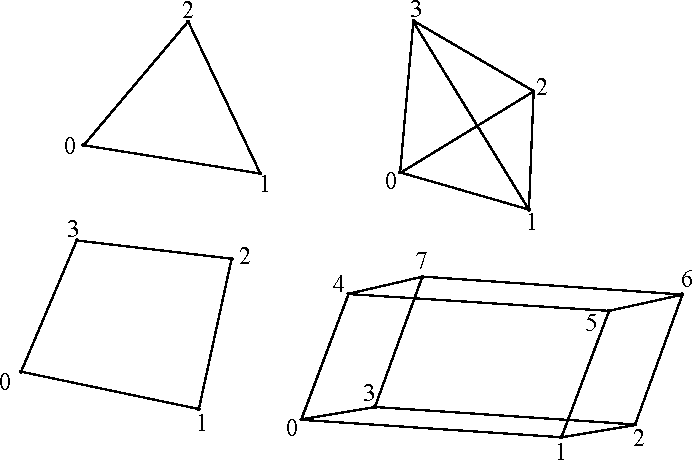
\includegraphics[width=10cm]{Elements}
\caption{Common element shapes. Left to right, top to bottom: triangle, tetrahedron, quadrilateral and hexahedron.}
\label{fig:Elements}
\end{figure}

\begin{figure}[h!]
\centering
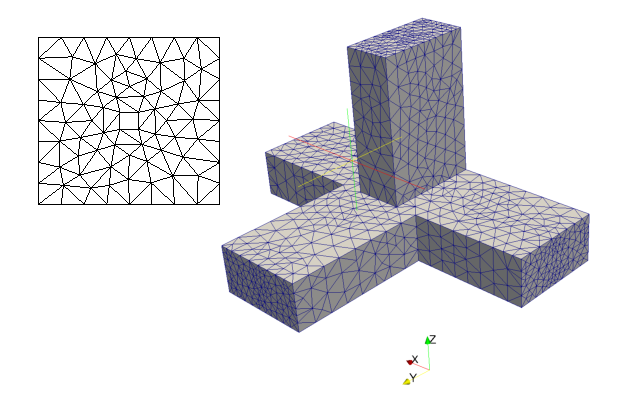
\includegraphics[width=12cm]{Mesh}
\caption{Finite element meshes. Left to right: triangularization a square domain surrounding a small square, tetrahedralization of microwave Magic-Tee.}
\label{fig:Mesh}
\end{figure}

As the mesh is used as the support for a piecewise linear approximation of a function, the accuracy of the approximation directly depends on the sizes and shapes of the elements. If the elements are small enough (typically less than $\frac{\lambda}{10}$ per side), then the field inside the element can be reliably approximated by linear polynomials. For greater dimensions, one may increase the polynomial order to achieve better approximation at the cost of an increase of the interpolation coefficients number.

The accuracy is also related to the elements shape and how far they are to be \quotes{regular} or equilateral: there is a mathematical connection between the mesh \quotes{quality}, the interpolation errors and the global matrix conditioning \cite{tsukerman1998comparison}. Low quality, \quotes{needle-like}, elements may increase the condition number of the system matrix (poor conditioning), and consequently, may cause a degradation in the accuracy of the results. There have been a lot of efforts in finding the best compromise between the generation of good quality mesh while containing the computational requirements. The most diffused approach is the adaptive mesh refinement ($h$-AMR), where appropriately chosen error indicators (mainly based on the gradient of the function) are used to refine locally higher error elements (next to metallic corners, discontinuities in material properties and any other potential singularity of the function) of the mesh \cite{sun2000adaptive,ingelstrom2004higher}. Other approaches are a combination of the elements refinements ($h$-refinements) and the polynomial orders refinements ($p$-refinements) which lead to a better compromise \cite{solin2010adaptive}.

FES package integrates, in the 2D form, the Triangle Mesh Generator \cite{shewchuk2002delaunay} and, in the 3D form, TetGen \cite{si2008three}. Both are based on the Delaunay triangulation which intrinsically allow for optimized mesh quality control, even for really complex geometries. Also, for validation purposes, meshes generated from commercial packages, Comsol (2D) and HFSS (3D), can be imported  in the analogous version of FES, restricting in such a way the errors to the steps of the finite element method following the mesh generation, mainly assembly and solve steps.


\subsection{Shape functions}

Accurate definition of the functional space of the solution is necessary to obtain physical solutions. In fact, the PDE with the necessary boundary conditions (initial conditions neglected for the time-harmonic assumption) treated until now, in a totally continuous space, are sufficient to prove existence and uniqueness of the solution. In a discretized world, this might not be true. However, one of the most important results of numerical solution of PDE is given by Cea's theorem \cite{ciarlet1978finite}, the equivalent functional analysis' Max-Milgram theorem, which in simple terms states that once one can prove that a linear operator (the PDE) on a specific functional space is bounded, then the numerical solution to the PDE exists and is unique within a bounded error (maximum error). Furthermore, as the finite discretization tends to the continuous case ($\mathcal{M}_h(\Omega) \rightarrow \Omega$), the error tends to vanish. This is the fundamental aspect of the finite elements: there is a convergence of the numerical solution to the exact solution. 

As a consequence, we need to provide the proper function spaces in which the operators for Maxwell's equations (curls, divergences, gradients) are bounded. We define the \quotes{boundedness} of the solution in $\Omega$ in terms of the Euclidean distance or, more generally, the Lebesgue space $\mathcal{L}^2(\Omega)$. Furthermore, we define the $D$-dimensional ($D := 2,3$) Lebesque space to be a Hilbert space in such a way that
$$\left (\mathcal{L}^2(\Omega)\right)^D = \left \lbrace \mathbf{v} : \Omega \rightarrow \mathbb{C}^D \ | \ \Vert \mathbf{v}\Vert_{(\mathcal{L}^2(\Omega))^D }  = \int_\Omega |\mathbf{v}|^2 d\Omega < \infty \right \rbrace.$$

To guarantee the boundedness of differential operators in vector spaces, we introduce some important Sobolev spaces \cite{monk2003finite}.

\subsubsection{\texorpdfstring{$\mathcal{H}^1(\Omega)$ Sobolev space}{H1 Sobolev space}}

One of the Sobolev spaces, related to all the square integrable functions that have square integrable gradient, is defined as

$$\mathcal{H}^1(\Omega) = \left \lbrace \phi \in \mathcal{L}^2(\Omega) \ | \ \nabla \phi \in (\mathcal{L}^2(\Omega))^D \right \rbrace,$$

\noindent with the norm

$$\Vert\phi\Vert_{\mathcal{H}^1(\Omega)} = \left( \Vert\phi\Vert_{\mathcal{L}^2(\Omega)}^2 + \Vert\nabla \phi\Vert_{(\mathcal{L}^2(\Omega))^D}^2 \right)^{1/2}.$$

\noindent As we will see, this is the \quotes{home} space for the electric field in 2D transversal magnetic formulation for the wave equation. This space and related formulations have been used extensively to assess the domain decomposition and nonlinear analyses of chapters \ref{chap:DD} and \ref{chap:NL}. More generally, this is the home for scalar potentials and for electric charge densities.

\subsubsection{\texorpdfstring{$\mathcal{H}(\mathrm{curl},\Omega)$ Sobolev space}{Hcurl Sobolev space}}

Another important Sobolev space, related to all the square integrable functions that have square integrable curl, is defined as
%
$$\mathcal{H}(\mathrm{curl},\Omega) = \left \lbrace \mathbf{v} \in (\mathcal{L}^2(\Omega))^D \ | \ \nabla  \times \mathbf{v} \in (\mathcal{L}^2(\Omega))^D \right\rbrace,$$
%
\noindent with the norm
%
$$\Vert\mathbf{v}\Vert_{\mathcal{H}(\mathrm{curl},\Omega)} = \left( \Vert \mathbf{v} \Vert_{(\mathcal{L}^2(\Omega))^D}^2 + \Vert\nabla \times \mathbf{v} \Vert_{(\mathcal{L}^2(\Omega))^D}^2 \right)^{1/2}.$$
%
\noindent This space fundamentally represents the electric and magnetic field intensities, $\mathbf{E}$ and $\mathbf{H}$, within Maxwell's equations.
%
\subsubsection{\texorpdfstring{$\mathcal{H}(\mathrm{div},\Omega)$ Sobolev space}{Hdiv Sobolev space}}
%
Another important Sobolev space, related to all the square integrable functions that have square integrable divergence, is defined as
%
$$\mathcal{H}(\mathrm{div},\Omega) = \left\lbrace \mathbf{v} \in (\mathcal{L}^2(\Omega))^D \ | \ \nabla  \cdot \mathbf{v} \in (\mathcal{L}^2(\Omega))^D \right\rbrace,$$
%
\noindent with the norm
%
$$\Vert\mathbf{v}\Vert_{\mathcal{H}(\mathrm{div},\Omega)} = \left( \Vert \mathbf{v} \Vert_{(\mathcal{L}^2(\Omega))^D}^2 + \Vert\nabla \cdot \mathbf{v} \Vert_{(\mathcal{L}^2(\Omega))^D}^2 \right)^{1/2}.$$
%
\noindent This space fundamentally represents the electric and magnetic inductions intensities, $\mathbf{D}$ and $\mathbf{B}$, and the electrical current density $\mathbf{J}$ within Maxwell's equations.
%
\subsubsection{de Rham complex}
%
Here comes an interesting result pertaining to the Sobolev spaces defined above: the vector identities $\nabla \times \nabla \phi = 0$ and $\nabla \cdot \nabla \times \mathbf{v} = 0$, where $\phi \in \mathcal{H}^1(\Omega)$ and $\mathbf{v} \in \mathcal{H}(\mathrm{curl},\Omega)$, can be used to establish a relationship between the spaces. For instance, in view of identity $\nabla \times \nabla \phi = 0$, $\nabla \phi \in \mathcal{H}(\mathrm{curl},\Omega)$ and $\nabla \cdot \nabla \times \mathbf{v} = 0$ implies $\nabla \times \mathbf{v} \in \mathcal{H}(\mathrm{div},\Omega)$. These relationships can be summarized as

$$\mathcal{H}^1(\Omega) \ \stackrel{\nabla}{  \longrightarrow} \ \mathcal{H}(\mathrm{curl},\Omega) \ \stackrel{ \nabla\times}{ \longrightarrow} \ \mathcal{H}(\mathrm{div},\Omega) \stackrel{\nabla\cdot}{ \longrightarrow} \ \mathcal{L}^2(\Omega),$$

\noindent and important mapping can be immediately visualized with this so-called de Rham complex: gradients map $\mathcal{H}^1(\Omega)$ to $\mathcal{H}(\mathrm{curl},\Omega)$ and curls map $\mathcal{H}(\mathrm{curl},\Omega)$ to $\mathcal{H}(\mathrm{div},\Omega)$. 

The electromagnetic quantities and their corresponding function space are shown in table \ref{tab:quantspace}.


\begin{table}[h!]
\begin{center}
\begin{tabular}{|c|c|}
\hline 
Quantity & Function space \\ 
\hline
\hline 
$\mathbf{E}, \mathbf{H}$ & $\mathcal{H}(\mathrm{curl},\Omega)$ \\ 
\hline 
$\mathbf{D}, \mathbf{B}, \mathbf{J}$ & $\mathcal{H}(\mathrm{div},\Omega)$ \\ 
\hline 
$\rho$ & $\mathcal{L}^2(\Omega)$ \\ 
\hline 
$\epsilon_0 \dyad{\epsilon}_r, \mu_0 \dyad{\mu}_r$ & $\mathcal{H}(\mathrm{curl},\Omega) \longrightarrow \mathcal{H}(\mathrm{div},\Omega)$ \\ 
\hline 
\end{tabular}
\end{center}
\caption{Electromagnetic quantities and their function space.}
\label{tab:quantspace}
\end{table}

\subsubsection{Scalar and rotational basis functions}

The basis functions chosen to expand the $\mathcal{H}^1(\Omega)$ space, especially tailored to expand scalar functions, are based on the simplex coordinates $\phi_i$ \cite{pelosi2009quick}. $\phi_i$ is the continuous function that is linear on each triangle or tetrahedron, being one at node $i$ and zero at all other nodes.

Each basis function is associated with either a node $\lbrace i \rbrace$, an edge $\lbrace ij \rbrace$, a triangular face $\lbrace ijk \rbrace$ or a tetrahedron $\lbrace ijkl \rbrace$ of the mesh.

The continuous, scalar ($\mathcal{H}^1(\Omega)$-conforming) finite element spaces of order $p$ are given by $\mathcal{V}^p = \mathcal{S}^1 \oplus \ldots \mathcal{S}^p$, where $\mathcal{S}^p \subset \mathcal{H}^1(\Omega)$ are given in table \ref{tab:H1functions}. We note that the functions in $\mathcal{V}^p$ are continuous across element boundaries.

\begin{table}[h!]
\begin{center}
\begin{tabular}{|c|c|c|}
\hline 
Space & Basis functions & Mesh entity \\ 
\hline
\hline 
$\mathcal{S}^1$ & $\phi_i$ & $\lbrace i \rbrace$ \\ 
\hline 
$\mathcal{S}^2$ & $\phi_i\phi_j$ & $\lbrace ij \rbrace$ \\ 
\hline 
$\mathcal{S}^3$ & $\phi_i\phi_j(\phi_i - \phi_j)$ & $\lbrace ij \rbrace$ \\ 
 & $\phi_i\phi_j\phi_k$ & $\lbrace ijk \rbrace$ \\ 
\hline 
\end{tabular} 
\end{center}
\caption{$\mathcal{H}^1(\Omega)$-conforming basis functions up to order $p = 3$.}
\label{tab:H1functions}
\end{table}


For the rotational basis functions, we have chosen to expand the $\mathcal{H}(\mathrm{curl},\Omega)$ with N\'ed\'elec incomplete order spaces \cite{nedelec1980mixed} which often lead to sparser matrices than the complete order counterpart while achieving approximately the same accuracy. They also permit the use of different elemental orders in a single finite element iterative solution with $p$-multilevel preconditioners \cite{sun2001construction}. The $\mathcal{H}(\mathrm{curl},\Omega)$-conforming finite element space of order $p$ is hence constructed recursively,

$$\mathcal{W}^p = \mathcal{W}^{p-1} \oplus \bar{\mathcal{W}}^{p} \ \mathrm{for} \ p = 2, 3 \ \mathrm{and} \ \mathcal{W}^{1}= \mathcal{R}^{1},$$

\noindent with the incremental space $\bar{\mathcal{W}}^p = \mathcal{R}^p \oplus \nabla \mathcal{S}^p$. The tangential components of $\mathcal{W}^p$ are continuous across element boundaries whereas the normal component may be discontinuous.

\begin{table}[h!]
\begin{center}
\begin{tabular}{|c|c|c|}
\hline 
Space & Basis functions & Mesh entity \\
\hline
\hline 
$\mathcal{R}^1$ & $\phi_i\nabla\phi_j-\phi_j\nabla\phi_j$ & $\lbrace ij \rbrace$ \\
\hline 
$\mathcal{R}^2$ & $3\phi_j\phi_k\nabla\phi_i-\nabla(\phi_i\phi_j\phi_k)$ & $\lbrace ijk \rbrace$ \\
 & $3\phi_k\phi_i\nabla\phi_j-\nabla(\phi_i\phi_j\phi_k)$ & $\lbrace ijk \rbrace$ \\
\hline 
$\mathcal{R}^3$ & $4\phi_j\phi_k(\phi_j - \phi_k)\nabla\phi_i - \nabla\left(\phi_i\phi_j\phi_k(\phi_j-\phi_k)\right)$ & $\lbrace ijk \rbrace$ \\
 & $4\phi_k\phi_i(\phi_k - \phi_i)\nabla\phi_j - \nabla\left(\phi_i\phi_j\phi_k(\phi_k-\phi_i)\right)$ & $\lbrace ijk \rbrace$ \\
 & $4\phi_i\phi_j(\phi_i - \phi_j)\nabla\phi_k - \nabla\left(\phi_i\phi_j\phi_k(\phi_i-\phi_j)\right)$ & $\lbrace ijk \rbrace$ \\
 & $4\phi_j\phi_k\phi_l\nabla\phi_i - \nabla(\phi_i\phi_j\phi_k\phi_l)$ & $\lbrace ijkl \rbrace$ \\ 
 & $4\phi_k\phi_l\phi_i\nabla\phi_j - \nabla(\phi_i\phi_j\phi_k\phi_l)$ & $\lbrace ijkl \rbrace$ \\ 
 & $4\phi_l\phi_i\phi_j\nabla\phi_k - \nabla(\phi_i\phi_j\phi_k\phi_l)$ & $\lbrace ijkl \rbrace$ \\ 
\hline 
\end{tabular} 
\end{center}
\caption{$\mathcal{H}(\mathrm{curl},\Omega)$-conforming basis functions up to order $p = 3$.}
\label{tab:Hcurlfunctions}
\end{table}

\subsection{Galerkin framework}

Among the finite element formulations, the Galerkin approach is the most straightforward to achieve finite element matrices. While the Rayleigh-Ritz approach requires to derive the proper Hamiltonian that describes the physics of the problem,  minimizing it, the Galerkin approach simply requires to define projections, which may be intrinsic from the definition of the shape functions in a Hilbert space. In fact, in a Hilbert space, the projection from a space to another is given by the Lebesgue scalar product 
%
$$<\mathbf{u},\mathbf{v}> = \int_\Omega \mathbf{u}^* \mathbf{v} \ d\Omega,$$
%
\noindent where $^*$ implies the adjoint operator (hermitian transpose). Furthermore, the original Galerkin projection is such that the space of origin $\mathcal{V}$ is the same of the arrival space $\mathcal{V}$. 

Consider the linear operator $A : \mathcal{V} \longrightarrow \mathcal{V}$, the corresponding homogeneous system is
$$A \mathbf{v} = \mathbf{f},$$
\noindent where $\mathbf{v} \in \mathcal{V}$ and $\mathbf{f} \in \mathcal{V}$. With the Galerkin approach, we seek $\mathbf{v} \in \mathcal{V}$ such that
$$< \mathbf{t}, A \mathbf{v}> = <\mathbf{t},\mathbf{f}>, \quad \forall \mathbf{t} \in \mathcal{V}.$$
\noindent Let us also assume the $N$-dimensional space $\mathcal{V}_h\in \mathcal{V}$ described by shape functions $\mathbf{v}_j$ such that $\mathbf{v}_h = \sum_{j=1}^N x_j \mathbf{v}_j$ and $\mathbf{t}_h = \mathrm{span}\lbrace{\mathbf{v}_1, \ldots, \mathbf{v}_i, \ldots, \mathbf{v}_n}\rbrace$. If we seek $\mathbf{v}_h \in \mathcal{V}_h$ such that
\begin{equation}
\sum_{i=1}^N x_j < \mathbf{v}_i, A \mathbf{v}_j> = <\mathbf{v}_i,\mathbf{f}>, \quad \forall \mathbf{v}_i, \ \ \ i=1,\ldots,N,
\label{eq:Galerkin}
\end{equation}
%
\noindent and, by Cae's theorem, $\mathbf{v}_h$ exists and is unique. The system \eqref{eq:Galerkin} can be turned into an $N$-dimensional set of linear equations whose solution is found by solving the $(N \times N)$-matrix system
$$ \mat{A} \ \vect{x} = \vect{b}.$$
The matrix entries $\mathrm{A}_{ij} = < \mathbf{v}_i, A \mathbf{v}_j>$, the source vector entries are $\mathrm{b}_i = <\mathbf{v}_i,\mathbf{f}>$ and the unknown $\vect{x}$ contains the expansion coefficients $x_j$ for the solution $\mathbf{v} \approx \mathbf{v}_h = \sum_{j=1}^N x_j \mathbf{v}_j$.


\subsubsection{Problem model}

Let us consider the domain $\Omega \subset \mathbb{R}^3$ to be bounded by $\mathrm{\partial \Omega = \Gamma = \Gamma_E \cup \Gamma_{H} \cup \Gamma_{WG} \cup \Gamma_R}$ for the antenna problem and by $\mathrm{\partial \Omega = \Gamma = \Gamma_E \cup \Gamma_{H} \cup \Gamma_R}$ for the scattering problem as depicted in figure \ref{fig:FEMproblem}.
\begin{figure}[hbpt!]
\centering
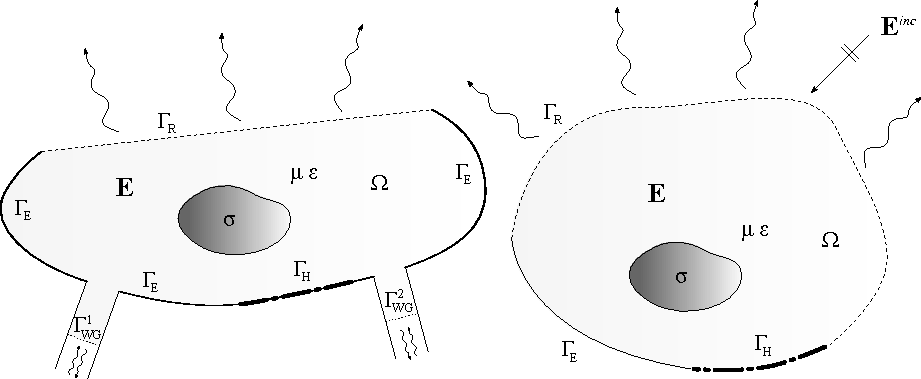
\includegraphics[width=12cm]{FEMproblem} 
\caption{Finite element domains for the antenna and the  scattering problems.}
\label{fig:FEMproblem}
\end{figure}

$\mathrm{\Gamma}_E$ corresponds to Dirichlet boundary conditions, $\mathrm{\Gamma}_H$ to Neumann boundary conditions, $\mathrm{\Gamma}_{WG}$ to mode matching boundary condition at waveguides ports, and $\mathrm{\Gamma}_R$ corresponds to Robin boundary conditions. The later, also known as \textit{impedance} or \textit{radiation} boundary, allow to mimic open problems. The antenna problem can be straightforwardly reduced to a closed waveguide device problem upon neglecting the radiation boundaries.

Consider now the discretized domain $\Omega_h = \bigcup_{n=1}^{N} \Omega_n \subset \Omega$, where the subdomains $\Omega_n$ (triangles or tetrahedra of the mesh) are such that $\Omega_n \cap \Omega_m = \{ \emptyset \}$ for $n \neq m$. $\Omega_h$ is parameterized in by the maximum dimension $h$ of the subdomains $\Omega_n$, and we shall assume that as $h \to 0$, $\Omega_h \to \Omega$ (the mesh is said to be conforming to the CAD model).

With $\hat{\mathbf{n}}$ pointing outwardly from $\Omega$, consider space $\mathcal{W} = \mathcal{W}(\Omega_h) \subset \mathcal{H}(\mathrm{curl}, \Omega)$ of the curl-conforming shape functions $\mathbf{w}$, defined by the direct sum of two closed subspaces as follows
\begin{eqnarray}
\mathcal{W} &= & \mathcal{W}_D \oplus \mathcal{W}_E, \nonumber \\[5pt]
\mathcal{W}_D &:= & \{ \mathbf{w} \in \mathcal{W} \ | \ \hat{\mathbf{n}} \times \mathbf{w} \neq 0 \ \mathrm{on} \ \mathrm{\Gamma}_E \} \subset \mathcal{H}(\mathrm{curl},\Omega), \nonumber \\
\mathcal{W}_E &:= & \{ \mathbf{w} \in \mathcal{W} \ | \ \hat{\mathbf{n}} \times \mathbf{w} = 0 \ \mathrm{on} \ \Gamma_E \} \subset \mathcal{H}(\mathrm{curl},\Omega, \Gamma_E).\nonumber
\end{eqnarray} $\mathcal{W}_D$ is in fact the subspace for the imposition of Dirichlet conditions. The total electric field is given by the approximating finite summations
\begin{eqnarray}
\label{eq:fieldExp}
\mathbf{E} & = & \mathbf{E}_E + \mathbf{E}_D, \nonumber \\[5pt]
\mathbf{E}_E &:= & \sum_{j=1}^{N} x_j \mathbf{w}_j, \qquad \mathbf{w}_j \in \mathcal{W}_E, \nonumber \\
\mathbf{E}_D&:= & \sum_{d=1}^{N^D} x_d \mathbf{w}_d, \qquad \mathbf{w}_d \in \mathcal{W}_D.\nonumber
\end{eqnarray} 

The PDE we must solve to retrieve the fields is \eqref{eq:waveeqE}, reported here for convenience
$$ \nabla \times \frac{1}{\mu_r} \nabla \times {\mathbf{E}} + j k_0 \zeta_0 \sigma {\mathbf{E}} - k_0^2 \epsilon_r {\mathbf{E}} =  0, $$

\noindent and the boundary conditions can be stated as
\begin{eqnarray}
\hat{\mathbf{n}} \times ( {\mathbf{E}} \times \hat{\mathbf{n}}) & = & \bar{\mathbf{E}}_t, \qquad \qquad \qquad \qquad \! \mathrm{on} \ \mathrm{\Gamma}_E, \\
\hat{\mathbf{n}} \times ( {\mathbf{H}} \times \hat{\mathbf{n}}) & = & \bar{\mathbf{H}}_t, \qquad \qquad \qquad \qquad \! \! \mathrm{on} \ \mathrm{\Gamma}_{H}, \\
\hat{\mathbf{n}} \times ( {\mathbf{E}} \times \hat{\mathbf{n}}) & = & Z_s {\mathbf{H}} \times \hat{\mathbf{n}}, \qquad \qquad \quad \ \  \mathrm{on} \ \mathrm{\Gamma}_R. \label{eq:ABC}%, \\
\end{eqnarray} 

\noindent $\bar{\mathbf{E}}_t$ and $\bar{\mathbf{H}}_t$ are known electric field and magnetic field distributions. $Z_s$ is the wave impedance at the radiation boundary to mimic the Sommerfeld radiation condition
$$\lim_{r \to \infty} r \left( (\nabla \times \mathbf{E}) \times \hat{\mathbf{n}} + j k \mathbf{E}\right) = 0,$$
\noindent and hence is chosen as $Z_s = \zeta_0 \sqrt{\frac{\mu_r}{\epsilon_r}}$ on $\Gamma_R$. One consideration must be done on the condition \eqref{eq:ABC}. In fact, that condition impose total absorbing condition on $\Gamma_R$ only for waves impinging perpendicularly to the surface, and the absorbing condition behaves poorly as waves come with a different incident angle. This is why it is typically recommended to put these boundaries at least $\frac{\lambda}{4}$ away form the radiators in order to reduce the internal reflections that may appear. Other methods have been employed to reduce this effect, such as increasing the order of the absorbing boundary condition \cite{jin2002finite} or, in a more rigorous way, employ boundary integral equations \cite{silvester1996finite} to totally absorb the fields from any incident angle.

We proceed with the Galerkin projections, testing with $\mathbf{w}_i \in \mathcal{W}_E$
$$ \int_\Omega \mathbf{w}_i^* \cdot \left ( \nabla \times \frac{1}{\mu_r} \nabla \times {\mathbf{E}} + j k_0 \zeta_0 \sigma {\mathbf{E}} - k_0^2 \epsilon_r {\mathbf{E}} \right) d\Omega =  0. $$
\noindent We integrate by parts the first term 
\begin{equation}
\label{eq:weakform}
\int_\Omega \mathbf{w}_i^* \cdot \nabla \times \frac{1}{\mu_r} \nabla \times {\mathbf{E}} \ d\Omega = \int_\Omega \nabla \times \mathbf{w}_i^* \cdot \frac{1}{\mu_r} \nabla \times {\mathbf{E}} \ d\Omega - \int_\Gamma \mathbf{w}_i^*  \times \frac{1}{\mu_r} \nabla \times {\mathbf{E}} \cdot \hat{\mathbf{n}} \ d\Gamma,
\end{equation}
\noindent and use of Faraday's law for the last right-hand side term
$$  - \int_\Gamma \mathbf{w}_i^*  \times \frac{1}{\mu_r} \nabla \times {\mathbf{E}} \cdot \hat{\mathbf{n}} \ d\Gamma = jk_0\zeta_0 \int_\Gamma \mathbf{w}_i^* \times \mathbf{H} \cdot \hat{\mathbf{n}} \ d\Gamma.$$
\noindent Evaluating the integrals on boundaries separately, we have
%
\begin{eqnarray}
\label{eq:Gamma}
jk_0\zeta_0 \int_\Gamma \mathbf{w}_i^*  \times \mathbf{H} \cdot \hat{\mathbf{n}} \ d\Gamma & = & jk_0\zeta_0 \int_{\Gamma_E} \hat{\mathbf{n}} \times \mathbf{w}_i^* \cdot \mathbf{H} \ d\Gamma \ + \nonumber \\
& & jk_0\zeta_0 \int_{\Gamma_H} \mathbf{w}_i^*  \times \mathbf{H} \cdot \hat{\mathbf{n}} \ d\Gamma \ + \nonumber \\
& & jk_0\zeta_0 \int_{\Gamma_R} \mathbf{w}_i^*  \times \mathbf{H} \cdot \hat{\mathbf{n}} \ d\Gamma,
\end{eqnarray}
%
\noindent where we have used the vector identities $\mathbf{A}\times\mathbf{B}\cdot\mathbf{C} = \mathbf{B}\times\mathbf{C}\cdot\mathbf{A} = \mathbf{C}\times\mathbf{A}\cdot\mathbf{B}$ for the first right-hand side integral, which results to be null as the testing functions are null on $\Gamma_E$. The magnetic field on $\Gamma_H$ can be decomposed as
$$\mathbf{H} = \bar{\mathbf{H}}_t + H_n \hat{\mathbf{n}} $$
\noindent hence the integral on $\Gamma_H$ can be reduced to
$$jk_0\zeta_0 \int_{\Gamma_H} \mathbf{w}_i^*  \times \mathbf{H} \cdot \hat{\mathbf{n}} \ d\Gamma = -jk_0\zeta_0 \int_{\Gamma_H} \mathbf{w}_i^*  \cdot \hat{\mathbf{n}} \times \bar{\mathbf{H}}_t \ d\Gamma.$$
\noindent The previous vector identity can be used, in conjunction with the radiation boundary condition, to recast the integral on $\Gamma_R$ as
\begin{eqnarray*}
jk_0\zeta_0 \int_{\Gamma_R} \mathbf{w}_i^*  \times \mathbf{H} \cdot \hat{\mathbf{n}} \ d\Gamma &= & jk_0\zeta_0 \int_{\Gamma_R} \frac{1}{Z_s}\hat{\mathbf{n}} \times (\mathbf{E} \times \hat{\mathbf{n}}) \cdot \mathbf{w}_i^* \ d\Gamma\\
&=& jk_0\zeta_0 \int_{\Gamma_R} \hat{\mathbf{n}} \times \mathbf{w}_i^* \cdot \frac{1}{Z_s}\hat{\mathbf{n}} \times \mathbf{E} \ d\Gamma
\end{eqnarray*}
\noindent We finally obtain the following weak form
\begin{multline}
\label{eq:FEMform}
\int_\Omega \nabla \times \mathbf{w}_i^* \cdot \frac{1}{\mu_r} \nabla \times \mathbf{E} \ d\Omega +
 j k_0 \zeta_0 \int_\Omega \mathbf{w}_i^* \cdot \sigma \mathbf{E} \ d\Omega \ + 
 j k_0 \zeta_0 \int_{\mathrm{\Gamma}_R} \hat{\mathbf{n}} \times \mathbf{w}_i^* \cdot \frac{1}{Z_s} \hat{\mathbf{n}} \times \mathbf{E} \ d\mathrm{\Gamma} \ - \\
 k_0^2 \int_\Omega \mathbf{w}_i^* \cdot \epsilon_r \mathbf{E} \ d\Omega \ = 
 j k_0 \zeta_0 \int_{\Gamma_{H}} \mathbf{w}_i^* \cdot \hat{\mathbf{n}} \times \bar{\mathbf{H}}_t \ d\Gamma - 
\int_\Omega \nabla \times \mathbf{w}_i^* \cdot \frac{1}{\mu_r} \nabla \times \mathbf{E}_D \ d\Omega \ - \\
j k_0 \zeta_0 \int_\Omega \mathbf{w}_i^* \cdot \sigma \mathbf{E}_D \ d\Omega +
 k_0^2 \int_\Omega \mathbf{w}_i^* \cdot \epsilon_r \mathbf{E}_D \ d\Omega, 
\qquad \forall \mathbf{w}_i \in \mathcal{W}_E.
\end{multline}
\noindent In practical microwave applications, the Dirichlet boundary condition is generally associated to perfect electric conductors where we have $\bar{\mathbf{E}}_t = 0$ ($\mathbf{E}_D = 0$) while the Neumann boundary condition corresponds to perfect magnetic conductors with $\bar{\mathbf{H}}_t = 0$. This implies the right-hand side of \eqref{eq:FEMform} vanishes. Thus, the source vector must be supplied by either waveports modal field distributions on $\Gamma_{WG}$, for the antenna or the waveguide device, or the impinging external field on $\Gamma_R$, for the scattering problem.

\subsubsection{Waveports boundary conditions}

In order to supply excitation on $\Gamma_{WG}$ two approaches can be employed: the radiation conditions on ports or the transfinite element method. The first is somehow less accurate than the second one, but less computationally involving and easy to implement.

%Both the approaches need that the waveguide segments on which the wave ports are applied to be long enough such that the higher order modes are evanescent and once they encounter the electromagnetic structure's discontinuities (e.g. the junction to the antenna) their power contribution is several order of magnitude lower than the one of the dominant mode.

\subsubsection*{Dominant mode continuity}

This approach limits the analysis in $\Omega$ to the accuracy provided by considering only the dominant modes to be incident on $\Gamma_{WG}$ and somehow considering an equivalent radiation condition to absorb the back-scattered field. It is mandatory, for accurate modeling of the problems, that the boundaries are located sufficiently far form any discontinuity, such that any back-scattered higher order mode, evanescent in the waveguide, has vanished (several orders of magnitude lower than the dominant mode) once back at the boundary.

On $\Gamma_{WG}$, if we consider the wave ports to be fed only by a $k^\mathrm{th}$ dominant mode (lowest cut-off frequency), the following relation holds for the port \cite{pelosi2009quick, zhu2006multigrid}
\begin{eqnarray}
\label{eq:WGcond}
\hat{\mathbf{n}} \times \mathbf{H}_t^k & = & \frac{1}{Z_k} \hat{\mathbf{n}} \times \hat{\mathbf{n}} \times \mathbf{E}_t^k - \frac{2}{Z_k} \hat{\mathbf{n}} \times \hat{\mathbf{n}} \times \mathbf{E}_t^{k \ inc}, \qquad \mathrm{on} \ \Gamma_{WG}^k,
\end{eqnarray} where $\mathbf{E}_t^{k \ inc}$ is the incident electric field and ${Z_k}$ the modal impedance. By analogy with the previous formulation for $\Gamma_H$ \eqref{eq:Gamma}, \eqref{eq:FEMform} becomes 
\begin{eqnarray}
\label{eq:FEMformRadPorts}
& & \hspace{-1.5cm} \int_\Omega \nabla \times \mathbf{w}_i^* \cdot \frac{1}{\mu_r} \nabla \times \mathbf{E} \ d\Omega + j k_0 \zeta_0 \int_\Omega \mathbf{w}_i^* \cdot \sigma \mathbf{E} \  d\Omega \ - \nonumber \\
& &\hspace{-1cm} k_0^2 \int_\Omega \mathbf{w}_i^* \cdot \epsilon_r \mathbf{E} \ d\Omega + j k_0 \zeta_0 \int_{\Gamma_R} \hat{\mathbf{n}} \times \mathbf{w}_i^* \cdot \frac{1}{Z_s} \hat{\mathbf{n}} \times \mathbf{E}\  d\Gamma + \nonumber \\
& & \hspace{-.5cm} j k_0 \zeta_0 \sum_{m=1}^{N^M} \int_{\Gamma_{WG}^m} \hat{\mathbf{n}} \times \mathbf{w}_i^* \cdot \frac{1}{Z_m} \hat{\mathbf{n}} \times \mathbf{E}_t^m \ d\Gamma \nonumber \\
& & \hspace{0cm} = j 2 k_0 \zeta_0 \int_{\Gamma_{WG}^k} \hat{\mathbf{n}} \times \mathbf{w}_i^* \cdot \frac{1}{Z_k} \hat{\mathbf{n}} \times \mathbf{E}_t^{k \ inc} \  d\Gamma, \qquad \forall \mathbf{w}_i \in \mathcal{W}_E
\end{eqnarray} where $N^M$ is the total number of modes and $k = 1, \ldots,  N^M$. Each of the $N^M$ modes, or a combination of them, can be used as excitation, leading to a non-null right-hand side in the finite element system. Notice that the modal field distributions $\mathbf{E}_t^m$ and relative impedance can be supplied either analytically or computed with a 2D eigenvalue problem (see below the transverse-longitudinal field formulation). The resulting system is
\begin{eqnarray}
\label{eq:inSystem}
\mat{A} \ \vect{x}  & = & \vect{b},
\end{eqnarray} where $\mat{A} \in \mathbb{C}^{N \times N}$, $\vect{x}$ and $\vect{b} \in \mathbb{C}^{N}$ with $N$ the number of unknowns equal to the number of shape functions $\mathbf{w}_j \in \mathcal{W}_E$. If materials within $\Omega$ are isotropic, then $\mat{A}$ is symmetric positive definite, enabling the use of memory-efficient solvers.

To retrieve scattering coefficients, one must compute, in the postprocessing phase, the following testings
$$S_{mk} = \frac{1}{2} \int_{\Gamma_{WG}^m}  \mathbf{E}^* \cdot \frac{1}{Z_m} \mathbf{E}_t^{m \ inc} \ d\Gamma - \delta_{mk}, \qquad m = 1, \ldots,  N^M,$$
\noindent where $\delta_{mk}$ is Kronecker's delta.

\subsubsection*{Transfinite element method}

The transfinite element method is more accurate in the way that better orthogonality between modes is enforced. On $\Gamma_{WG}$, the tangential electric and magnetic fields can be expanded as
\begin{eqnarray}
{\mathbf{E}}_t & = & \hat{\mathbf{n}} \times ( {\mathbf{E}} \times \hat{\mathbf{n}}) \ = \ \sum_{k} \left ( a_k^r + a_k^i \right ) \mathbf{E}_t^k, \qquad \, \mathrm{on} \ \mathrm{\Gamma}_{WG}, \\
{\mathbf{H}}_t & = & \hat{\mathbf{n}} \times ( {\mathbf{H}} \times \hat{\mathbf{n}}) \ = \ \sum_{k} \left ( a_k^r - a_k^i \right ) \mathbf{H}_t^k, \qquad \, \mathrm{on} \ \mathrm{\Gamma}_{WG},
\end{eqnarray} where $a_k^i, a_k^r$ the $k^\mathrm{th}$ complex modal incident and reflected amplitudes. The first step of the transfinite element method is to collect the shape functions defined in $\Omega$ apart from the ones defined on $\Gamma_{WG}$ such that
\begin{eqnarray}
\mathcal{W}_I & := & \left\lbrace \mathbf{w} \in \mathcal{W} \ | \ \hat{\mathbf{n}} \times \mathbf{w} = 0 \ \mathrm{on} \ \Gamma_{WG} \right\rbrace,\\
\mathcal{W}_{WG} & := & \left\lbrace \mathbf{w} \in \mathcal{W} \ | \ \hat{\mathbf{n}} \times \mathbf{w} \neq 0 \ \mathrm{on} \ \Gamma_{WG} \right\rbrace.
\end{eqnarray}
\noindent Hence, the $k^\mathrm{th}$ mode on $\Gamma_{WG}$ can be expanded in terms of shape functions such that
\begin{equation}
\label{eq:modalExp}
\mathbf{E}_t^k = \sum_{i=1}^{N_{WG}^k} m_i^k \mathbf{w}_i, \qquad \mathbf{w}_i \in \mathcal{W}_{WG}.
\end{equation}
\noindent Let us suppose the coefficients $m_i^k$ to be known. Considering one mode impinging on the waveports at a time, the electric field in $\Omega$ can be decomposed in the sum
\begin{equation}
%\label{eq:basis}
\mathbf{E} = \sum_{j=1}^{N-N_{WG}} x_j \mathbf{w}_j + \sum_{m=1}^{N_M} a_m^r \mathbf{E}_t^m
+ a_k^i \mathbf{E}_t^k, \quad \mathbf{w}_j \in \mathcal{W}_I,
\end{equation}
\noindent while the tangential magnetic field on $\Gamma_{WG}$ becomes 
\begin{equation}
%\label{eq:basis}
\mathbf{H}_t = \sum_{m=1}^{N_M} a_m^r \mathbf{H}_t^m - a_k^i \mathbf{H}_t^k.
\end{equation}
\noindent $N_m$ is the total number of modes retained in modal expansion and $N_{WG} = \sum_{k=1}^{N_M} N_{WG}^k$ is the total number of shape functions pertaining to $\mathcal{W}_{WG}$. The accuracy of the formulation is due to fact the incident mode is absorbed in the modal summation, letting $a_k^r \leftarrow a_k^r + a_k^i$. It follows that
\begin{equation}
%\label{eq:basis}
\mathbf{E} = \sum_{j=1}^{N-N_{WG}} x_j \mathbf{w}_j + \sum_{m=1}^{N_M} a_m^r \mathbf{E}_t^m,
\end{equation}
\noindent and
\begin{equation}
%\label{eq:basis}
\mathbf{H}_t = \sum_{m=1}^{N_M} a_m^r \mathbf{H}_t^m - 2 a_k^i \mathbf{H}_t^k.
\end{equation}
\noindent Again, by analogy with \eqref{eq:Gamma}, the following weak form is optained \cite{zhu2006multigrid} 
%
\begin{multline}
\label{eq:FEMformTFE1}
\int_\Omega \nabla \times \mathbf{w}_i^* \cdot \frac{1}{\mu_r} \nabla \times \left( \sum_{j=1}^{N-N_{WG}} x_j \mathbf{w}_j + \sum_{m=1}^{N_M} a_m^r \mathbf{E}_t^m \right) \ d\Omega +\\
 j k_0 \zeta_0 \int_\Omega \mathbf{w}_i^* \cdot \sigma \left( \sum_{j=1}^{N-N_{WG}} x_j \mathbf{w}_j + \sum_{m=1}^{N_M} a_m^r \mathbf{E}_t^m \right) \ d\Omega \ + \\
 j k_0 \zeta_0 \int_{\mathrm{\Gamma}_R} \hat{\mathbf{n}} \times \mathbf{w}_i^* \cdot \frac{1}{Z_s} \hat{\mathbf{n}} \times \left( \sum_{j=1}^{N-N_{WG}} x_j \mathbf{w}_j + \sum_{m=1}^{N_M} a_m^r \mathbf{E}_t^m \right) \ d\mathrm{\Gamma} - \\
 k_0^2 \int_\Omega \mathbf{w}_i^* \cdot \epsilon_r \left( \sum_{j=1}^{N-N_{WG}} x_j \mathbf{w}_j + \sum_{m=1}^{N_M} a_m^r \mathbf{E}_t^m \right) \ d\Omega \ = \\ 
 j k_0 \zeta_0 \int_{\Gamma_{WG}}  \mathbf{w}_i^* \cdot \hat{\mathbf{n}} \times \left( \sum_{m=1}^{N_M} a_m^r \mathbf{H}_t^m - 2 a_k^i \mathbf{H}_t^k \right) \ d\Gamma, \qquad \forall \mathbf{w}_i \in \mathcal{W}_I\cap \mathcal{W}_E,
\end{multline}
\noindent having considered $\Gamma_E$ to be on perfect electric conductor and $\Gamma_H$ on perfect magnetic conductor. Since the testing shape functions $\mathbf{w}_i$ have been excluded from $\mathcal{W}_{WG}$, the right-hand side integral vanishes and the resulting system of equations is given by
\begin{equation}
\label{eq:FEInt1}
\mat{P} \vect{x_{WG}} + \mat{A} \vect{x_I} = \vect{0},
\end{equation}
\noindent where $\vect{x_{WG}}$ is a vector corresponding to reflected modal amplitudes on $\Gamma_{WG}$ and $\vect{x_I}$ is the unknown vector corresponding to the shape functions internal to $\Omega / \Gamma_{WG}$.

At this point, no excitation is provided yet. We need to supply further testings with the modal expansions \eqref{eq:modalExp}, such that

\begin{multline}
\label{eq:FEMformTFE2}
\int_\Omega \nabla \times \mathbf{E}_t^{i*} \cdot \frac{1}{\mu_r} \nabla \times \left( \sum_{j=1}^{N-N_{WG}} x_j \mathbf{w}_j + \sum_{m=1}^{N_M} a_m^r \mathbf{E}_t^m \right) \ d\Omega +\\
 j k_0 \zeta_0 \int_\Omega \mathbf{E}_t^{i*} \cdot \sigma \left( \sum_{j=1}^{N-N_{WG}} x_j \mathbf{w}_j + \sum_{m=1}^{N_M} a_m^r \mathbf{E}_t^m \right) \ d\Omega \ + \\
 j k_0 \zeta_0 \int_{\mathrm{\Gamma}_R} \hat{\mathbf{n}} \times \mathbf{E}_t^{i*} \cdot \frac{1}{Z_s} \hat{\mathbf{n}} \times \left( \sum_{j=1}^{N-N_{WG}} x_j \mathbf{w}_j + \sum_{m=1}^{N_M} a_m^r \mathbf{E}_t^m \right) \ d\mathrm{\Gamma} - \\
 k_0^2 \int_\Omega \mathbf{E}_t^{i*} \cdot \epsilon_r \left( \sum_{j=1}^{N-N_{WG}} x_j \mathbf{w}_j + \sum_{m=1}^{N_M} a_m^r \mathbf{E}_t^m \right) \ d\Omega \ = \\ 
 j k_0 \zeta_0 \int_{\Gamma_{WG}}  \mathbf{E}_t^{i*} \cdot \hat{\mathbf{n}} \times \left( \sum_{m=1}^{N_M} a_m^r \mathbf{H}_t^m - 2 a_k^i \mathbf{H}_t^k \right) \ d\Gamma, \qquad i = 1, \ldots, N_m.
\end{multline}
\noindent Now the integrals with $\mathbf{w}_j$ vanish,  as their subspace is orthogonal to the subspace of the testing functions $\mathbf{E}_t^i$, that is $\mathcal{W}_I \perp \mathcal{W}_{WG}$. The right-hand side can be also written as
\begin{multline}
 j k_0 \zeta_0 \int_{\Gamma_{WG}}  \mathbf{E}_t^{i*} \cdot \hat{\mathbf{n}} \times \left( \sum_{m=1}^{N_M} a_m^r \mathbf{H}_t^m - 2 a_k^i \mathbf{H}_t^k \right) \ d\Gamma = \\
- j k_0 \zeta_0 \int_{\Gamma_{WG}} \mathbf{E}_t^{i*} \times  \sum_{m=1}^{N_M} a_m^r \mathbf{H}_t^m  \cdot \hat{\mathbf{n}} \ d\Gamma \ + \\
j 2 k_0 \zeta_0 \int_{\Gamma_{WG}} \mathbf{E}_t^{i*}  \times  a_k^i \mathbf{H}_t^k \cdot \hat{\mathbf{n}} \ d\Gamma
\end{multline}
\noindent By the use of orthonormal identity of the transverse modes
\begin{equation}
\int_{\Gamma_{WG}^p} \mathbf{E}_t^{p*}  \times  \mathbf{H}_t^q  \cdot \hat{\mathbf{n}} \ d\Gamma = \delta_{pq} \quad \mathrm{[W]}
\end{equation}
\noindent the follow system of equations is obtained
\begin{equation}
\label{eq:FEInt2}
\mat{R + \mathit{jk_\mathrm{0} \zeta_\mathrm{0}} I} \vect{x_{WG}} + \mat{P}^T \vect{x_I} = \vect{f},
\end{equation}
\noindent where $\mat{R}$ is the matrix obtained by testing on ports, $\mat{I}$ is the identity matrix, and $\mat{f}$ is the column vector with non-null entry $j2 k_0\zeta_0 a_k^i$ corresponding to the non-null incident modal amplitude. $(\cdot)^T$ is the transposition operator. $a_k^i$ is usually chosen to be $1$ (corresponding to $1~\mathrm{[W]}$ of impinging power) in order to retrieve scattering parameters. Furthermore, multiple righ-hand sides can be used to enforce all the modes, one at a time, without need to modify the system matrices. For instance
$$\mat{f} = j2 k_0\zeta_0 \mat{I}.$$
\noindent The full system can finally be cast as
\begin{equation}
\label{eq:FEsys}
\begin{bmatrix}
R + jk_0\zeta_0 I & P^T\\
P & A
\end{bmatrix}
\begin{bmatrix}
x_{WG} \\
x_{I}
\end{bmatrix} =
\begin{bmatrix}
j2 k_0\zeta_0 I \\
0
\end{bmatrix},
\end{equation}
%
\noindent where $x_I = \left[ x_1, \ldots, x_{N-N_{WG}} \right]^T$ are the unknowns internal to $\Omega/\lbrace\Gamma_{WG}\cup\Gamma_{E}\cup\Gamma_{H} \rbrace$, and $x_{WG} = \left[ a_1^r, \ldots, a_{N_m}^r \right]^T$ the complex-valued modal amplitudes for each mode.

Recalling the previously imposed absorbing condition for impinging mode, stated as (1 [W] of impinging power) $a_m^r \leftarrow a_m^r + \delta_{mk}$, the scattering parameters can be straightforwardly computed as
$$S_{mk} = a_m^r - \delta_{mk}, \qquad m = 1, \ldots,  N^M.$$
\noindent To compute the fields for a different impinging power, one might simply scale of the desired amount, $c = \sqrt{P^{inc}}$ with $P^{inc}$ the incident power, both $a_k^i \leftarrow c a_k^i$ and $a_k^r \leftarrow c (a_k^r+a_k^i)$. The power balance of the formulation is such that the scattering parameters remain the same.

A simple manner to assemble \eqref{eq:FEsys} is first to collect all the finite element coefficients pertaining to $\Omega$ apart from those on $\Gamma_{WG}$ such that
\begin{equation}
\begin{bmatrix}
A_{WG,WG} & A_{WG,I}\\
A_{I,WG} & A_{I,I}
\end{bmatrix}.
\end{equation}
\noindent Then, the expansion coefficients \eqref{eq:modalExp} of each mode, which can be viewed as column vectors 
$$\vect{m_k} = \left[m_1^k, \ldots, m_{N_{WG}^k} \right]^T,$$ 
\noindent and can be collected in a matrix $$\mat{M} = \left[\vect{m_1}, \ldots, \vect{m_{N_{M}}} \right] \ \in \mathbb{C}^{N_{WG} \times N_M}.$$
\noindent The system matrix \eqref{eq:FEsys} is finally obtained by computing
\begin{equation}
\label{eq:EqSysTFE}
\begin{bmatrix}
M^T A_{WG,WG} M + jk_0\zeta_0 I  & M^T A_{WG,I}\\
A_{I,WG} M & A_{I,I}
\end{bmatrix}
\begin{bmatrix}
x_{WG} \\
x_{I}
\end{bmatrix} =
\begin{bmatrix}
j2 k_0\zeta_0 I \\
0
\end{bmatrix}.
\end{equation}
\noindent It is evident that \eqref{eq:EqSysTFE} can be complex valued (due to waveports and radiation boundaries or material losses in terms of non null conductivity or complex permittivity and permeability), but a key point is the symmetry, if the same assumption of isotropic materials stands, which enables the use of memory-efficient matrix solvers.

\subsubsection*{Transverse-longitudinal field formulation}

The impinging modal field distributions in both dominant mode and transfinite element methods can be supplied by an analytical approach, when the geometry of $\Gamma_{WG}$ is rather simple and an expansion is already available. When the geometry gets complicated or the contour boundaries are not simply perfect electric or magnetic but radiating, computations becomes much more involving. Also, non homogeneous materials lead to difficult modal distributions computations.

A versatile way to compute the mode amplitudes is to solve an eigenvalue problem by the use of the finite element method, allowing thus to manage arbitrary geometries with arbitrary materials and boundary conditions. In the following, the transverse-longitudinal field formulation will be presented to compute the transverse fields used for waveports excitations.

\begin{figure}[hbpt!]
\centering
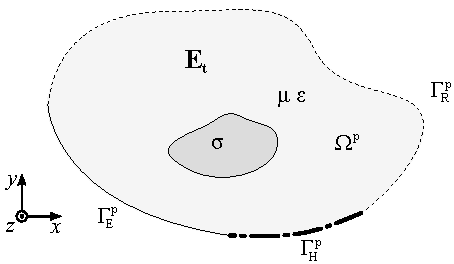
\includegraphics[width=8cm]{FEMproblemEigen} 
\caption{Finite element domain for the waveport eigenvalue problem.}
\label{fig:FEMproblemEigen}
\end{figure}

The electric field distribution $\mathbf{E}$ (at port $p$ on $\Gamma_{WG}$) is computed numerically by solving a \mbox{2-D}\footnote{Similar considerations can be done for $\Omega \equiv \Gamma_{WG}^p \in \mathbb{R}$ to compute excitations in FES-2D.} eigenvalue problem on $\Omega \equiv \Gamma_{WG}^p \in \mathbb{R}^2$ (Fig. \ref{fig:FEMproblemEigen}) using transverse-longitudinal field formulation \cite{zhu2006multigrid}. First, the electric field is expressed as the sum of transverse and longitudinal parts
\begin{equation}
\mathbf{E} = [\mathbf{E}_{t}(x,y) + \hat{\mathbf{z}} \ E_{z}(x,y)] \ \text{e}^{-\gamma z} \quad \text{on } \Omega,
\end{equation}
%
\noindent with $\hat{\mathbf{z}} = -\hat{\mathbf{n}}|_p$ and $\gamma$ is the propagation constant. After the definition of the vector basis functions $\mathbf{v} = \hat{\mathbf{n}}\times\vec{w} \in \mathcal{H}(\mathrm{curl}, \Omega^p, \Gamma_E)$ with $ \mathbf{w} \in \mathcal{W}_{WG} \cap \mathcal{W}_{E}$ such that $\mathbf{E}_{t} = \sum_{j=1}^{N_t} x_{t,j} \mathbf{v}_j$ and the scalar basis functions $\phi \in \mathcal{H}^1(\Omega^p, \Gamma_E)$ such that $E_{z} = \sum_{j=1}^{N_z} x_{z,j} \phi_j$, a Galerkin projection is applied to the eigenvalue problem with isotropic materials governed by
%
\begin{equation}
\nabla \times \frac{1}{\mu_r} \nabla \times \mathbf{E} - {k}_0^2 {\epsilon}_r \mathbf{E} = 0,
\end{equation}
%
\noindent with $\epsilon_r \leftarrow \epsilon_r + {\sigma}/{j\omega_0\epsilon_0}$, leading to the following generalized eigenvalue system of $N_t + N_z$ equations \cite{zhu2006multigrid,jiao2008fast}
\begin{equation}
\label{eq:eigen}
\begin{bmatrix}
{A}_{tt} &0\\
0 &0
\end{bmatrix}
\begin{bmatrix}
\gamma x_{t}\\
x_{z}
\end{bmatrix} = \ \gamma^2
\begin{bmatrix}
{B}_{tt} &{B}_{tz}\\
{B}_{zt} &{B}_{zz}
\end{bmatrix}
\begin{bmatrix}
\gamma x_{t}\\
x_{z}
\end{bmatrix},
\end{equation}
%
\noindent where the matrices entries are given by
\begin{equation*}
\begin{aligned}
A_{tt,ij} &= \int_{\Omega_p} \nabla_t \times \mathbf{v}_i  \cdot \frac{1}{\mu_r} \nabla_t \times \mathbf{v} \ d\Omega \ - \\
 & \qquad k_0^2 \int_{\Omega_p} \mathbf{v}_i  \cdot \epsilon_r \mathbf{v}_j \ d\Omega \ + \\ 
&  \qquad \qquad j k_0 \zeta_0
\int_{\Gamma_R^p} \mathbf{v}_i  \cdot \frac{1}{Z_s} \mathbf{v}_j \ d\Gamma, \\
B_{tt,ij} &= \int_{\Omega_p} \mathbf{v}_i  \cdot  \frac{1}{\mu_r}\mathbf{v}_j \ d\Omega, \\
B_{tz,ij} &= \int_{\Omega_p} \mathbf{v}_i  \cdot  \frac{1}{\mu_r}\nabla_t \phi_j \ d\Omega, \\
B_{zt,ij} &= \int_{\Omega_p} \nabla_t \phi_i  \cdot  \frac{1}{\mu_r}\mathbf{v}_j \ d\Omega, \\
B_{zz,ij} &= \int_{\Omega_p} \nabla_t \phi_i  \cdot  \frac{1}{\mu_r}\nabla_t \phi_j \ d\Omega \ - \\
& \qquad k_0^2 \int_{\Omega_p} \phi_i \epsilon_r \phi_j \ d\Omega \ +\\
& \qquad \qquad j k_0 \zeta_0 \int_{\Gamma_R^p} \phi_i \frac{1}{Z_s} \phi_j \ d\Gamma.
\end{aligned}
\end{equation*}

\noindent $\nabla_t = \hat{\mathbf{x}} \frac{\partial}{\partial x} + \hat{\mathbf{y}} \frac{\partial}{\partial y}$ is the transverse \textit{del} operator.
%

The eigenvalue problem \eqref{eq:eigen}, denoted as $\mat{A}\vect{x} = \lambda \mat{B}\vect{x}$, has $\mat{A}$ and $\mat{B}$ complex symmetric matrices due to the isotropic materials characteristics. The problem can then be solved with a Lanczos-based Krylov subspace solver \cite{farle2004finite} such as the public domain ARPACK solver	\cite{lehoucq1998arpack} in the \textit{shift-invert} mode operation
%
\begin{gather}
\mat{ A-\tau B }^{-1} \mat{B} \vect{x} =  \frac{1}{\lambda-\tau} \vect{x}, \nonumber \\[5pt]
\begin{aligned}
\tau &= k_0^2 \ \epsilon_\text{max} \ \mu_\text{max}, \\
\{\epsilon,\mu\}_\text{max} &= \max\limits_{(x,y)\in\Omega_p} \mathfrak{Re}\left( \{\epsilon,\mu\}(x,y) \right).
\end{aligned} \nonumber
\end{gather}
%
\noindent The shift-invert mode expedites the convergence of the employed iterative process when seeking for largest eigenvalues (lowest cut-off frequencies). Furthermore, spurious modes removal is performed by explicit imposition of $\mat{B}$-orthogonality of the Ritz vectors during the iterative process
%
$$
x_{z}  = - B_{zz}^{-1} B_{zt} \ \gamma x_{t}.
$$
%
Then, the $k^\mathrm{th}$ mode distribution $\mathbf{E}^k$ is normalized such that
%
$$
\int_{\Omega_p}  \mathbf{E}^{k*}  \times  \mathbf{H}^k  \cdot \hat{z} \ d\Omega = 1,
$$
%
\noindent which is achieved upon scaling the unknowns vector such that 
$$ \vect{x} \longleftarrow \frac{\vect{x}}{\sqrt{ \vect{x}^* \mat{B} \vect{x}} }.$$

\subsubsection{Total field scattering}

In this section, the total field scattering formulation is presented in order to treat the electromagnetic scattering from incident waves. We recall the formulation \eqref{eq:FEMform} to incorporate the incident field on the radiation boundary $\Gamma_R$
\begin{multline}
\label{eq:FEMformScatt1}
\int_\Omega \nabla \times \mathbf{w}_i^* \cdot \frac{1}{\mu_r} \nabla \times \mathbf{E} \ d\Omega +
 j k_0 \zeta_0 \int_\Omega \mathbf{w}_i^* \cdot \sigma \mathbf{E} \ d\Omega \ - \\ 
 k_0^2 \int_\Omega \mathbf{w}_i^* \cdot \epsilon_r \mathbf{E} \ d\Omega \ = 
 j k_0 \zeta_0 \int_{\Gamma_{R}} \mathbf{w}_i^* \cdot \hat{\mathbf{n}} \times \mathbf{H} \ d\Gamma, \qquad \forall \mathbf{w}_i \in \mathcal{W}_E.
\end{multline}
%
\noindent The electric and magnetic fields in $\Omega$ can be expressed as the sum of scattered part and an incident part
$$\mathbf{E} = \mathbf{E}^{sc} + \mathbf{E}^{inc}, \qquad \mathbf{H} = \mathbf{H}^{sc} + \mathbf{H}^{inc} $$
\noindent Direct substitution in \eqref{eq:ABC} where the $\mathbf{E} := \mathbf{E}^{sc}$ and $\mathbf{H} := \mathbf{H}^{sc}$ leads to
\begin{eqnarray}
\label{eq:IncBnd}
\hat{\mathbf{n}} \times \mathbf{H} & = & \frac{1}{Z_s} \hat{\mathbf{n}} \times \hat{\mathbf{n}} \times \mathbf{E} + \hat{\mathbf{n}} \times \mathbf{H}^{inc} - \frac{1}{Z_s} \hat{\mathbf{n}} \times \hat{\mathbf{n}} \times \mathbf{E}^{inc}, \qquad \mathrm{on} \ \Gamma_{R}.
\end{eqnarray}
\noindent The first term in right-hand side of \eqref{eq:IncBnd} leads to a radiation boundary integral (canonical first order absorbing boundary condition) while the next two terms will enforce the impinging field values on $\Gamma_R$. As a result
\begin{multline}
\label{eq:FEMformScatt}
\int_\Omega \nabla \times \mathbf{w}_i^* \cdot \frac{1}{\mu_r} \nabla \times \mathbf{E} \ d\Omega + j k_0 \zeta_0 \int_\Omega \mathbf{w}_i^* \cdot \sigma \mathbf{E} \ d\Omega \ + \\
\hspace{-2cm} j k_0 \zeta_0 \int_{\mathrm{\Gamma}_R} \hat{\mathbf{n}} \times \mathbf{w}_i^* \cdot \frac{1}{Z_s} \hat{\mathbf{n}} \times \mathbf{E} \ d\mathrm{\Gamma} \ - 
 k_0^2 \int_\Omega \mathbf{w}_i^* \cdot \epsilon_r \mathbf{E} \ d\Omega \ = \\
 j k_0 \zeta_0 \int_{\Gamma_{R}} \hat{\mathbf{n}} \times \mathbf{w}_i^* \cdot \left( \frac{1}{Z_s} \hat{\mathbf{n}} \times \mathbf{E}^{inc} - \mathbf{H}^{inc} \right) \ d\Gamma, \qquad \forall \mathbf{w}_i \in \mathcal{W}_E.
\end{multline}

\noindent The knowledge of the tangential components of the impinging wave on $\Gamma_R$ is sufficient to compute the total fields in $\Omega$. 
%If we consider a plane wave impinging 


\subsection{Element matrices and system assembly}

Efficient computation \cite{rognes2009efficient} of higher-order finite element matrices can be achieved by quadrature integration, and  mappings of the functions from a reference element to the actual element are used to recover the correct shape functions.

\begin{figure}[h!]
\centering
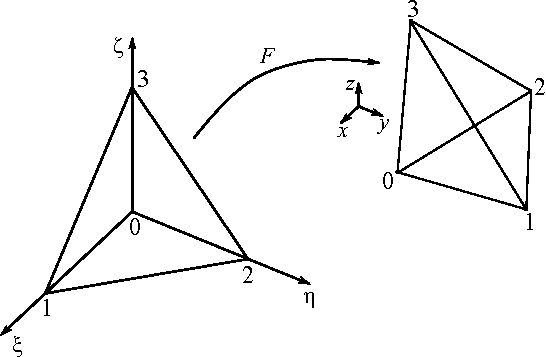
\includegraphics[width=10cm]{MappingTet}
\caption{Linear mapping $F$ of the reference element to the actual element.}
\label{fig:MappingTet}
\end{figure}

Consider the reference and actual elements of Fig. \ref{fig:MappingTet}. There exist a non degenerate affine mapping $F : K_0 \rightarrow K$ from the reference element $K_0$, defined in simplex coordinates $(\xi, \eta, \zeta)$ coordinates, the actual element $K$, defined Cartesian coordinates $(x,y,z)$, defined as
\begin{equation}
\label{eq:mapping}
\begin{bmatrix}
x\\y\\z
\end{bmatrix}
=
\begin{bmatrix}
x_1-x_0 & x_2-x_0 & x_3-x_0\\
y_1-y_0 & y_2-y_0 & y_3-y_0\\
z_1-z_0 & z_2-z_0 & z_3-z_0
\end{bmatrix}
\begin{bmatrix}
\xi \\ \eta \\ \zeta
\end{bmatrix}
+
\begin{bmatrix}
x_0\\
y_0\\
z_0
\end{bmatrix}.
\end{equation}

\noindent The Jacobian matrix $\mat{J}$ of the transformation, defined as
\begin{equation}
\label{eq:jacobian}
\begin{bmatrix}
J
\end{bmatrix}
=
\begin{bmatrix}
\frac{\partial x}{\partial \xi} & \frac{\partial y}{\partial \xi} & \frac{\partial z}{\partial \xi}\\
\frac{\partial x}{\partial \eta} & \frac{\partial y}{\partial \eta} & \frac{\partial z}{\partial \eta}\\
\frac{\partial x}{\partial \zeta} & \frac{\partial y}{\partial \zeta} & \frac{\partial z}{\partial \zeta}
\end{bmatrix},
\end{equation}

\noindent allows for straightforward computation of the partial derivatives of the shape functions: given a scalar function $\phi(\xi, \eta, \zeta)$ on the reference element, its partial derivatives on the actual element can be computed as
\begin{equation}
\label{eq:gradients}
\begin{bmatrix}
\frac{\partial \phi(x, y, z)}{\partial x} \\
\frac{\partial \phi(x, y, z)}{\partial y} \\
\frac{\partial \phi(x, y, z)}{\partial z} 
\end{bmatrix}
=
\begin{bmatrix}
J
\end{bmatrix}^{-1}
\begin{bmatrix}
\frac{\partial \phi(\xi, \eta, \zeta)}{\partial \xi} \\
\frac{\partial \phi(\xi, \eta, \zeta)}{\partial \eta} \\
\frac{\partial \phi(\xi, \eta, \zeta)}{\partial \zeta} 
\end{bmatrix}.
\end{equation}

\noindent Some of the integrals (the $\mathcal{H}(\mathrm{curl},\Omega)$-conforming \textit{stiffness} matrices) we have seen in the previous formulations involve the curls of the shape functions. They can readily be computed upon employing the vector identities $\nabla \times \left( \phi \mathbf{A} \right) = \phi \nabla \times \mathbf{A} + \nabla \phi \times \mathbf{A}$ and $\nabla \times \nabla \phi = 0$ and remembering that the curl operator is linear. The curls of the shape functions of table \ref{tab:Hcurlfunctions} can be recast in functions of the scalar functions and their gradients. Table \ref{tab:curlHcurlfunctions} shows their respective curls.

\begin{sidewaystable}[!]
\begin{center}
\begin{tabular}{|c|c|c|}
\hline 
Rotational basis $\left(\mathcal{H}(\mathrm{curl},\Omega)\right)$ & curl of rotational basis $\left(\mathcal{H}(\mathrm{div},\Omega)\right)$ \\
\hline
\hline 
$\phi_i\nabla\phi_j-\phi_j\nabla\phi_j$  & $2  (\nabla \phi_i \times \nabla \phi_j)$ \\
\hline 
$3\phi_j\phi_k\nabla\phi_i-\nabla(\phi_i\phi_j\phi_k)$ & $3 (\phi_j \nabla \phi_k +  \phi_k \nabla \phi_j ) \times \nabla \phi_i$ \\
$3\phi_k\phi_i\nabla\phi_j-\nabla(\phi_i\phi_j\phi_k)$ & $3 (\phi_k \nabla \phi_i + \phi_i \nabla \phi_k ) \times \nabla \phi_j$ \\
\hline 
$4\phi_j\phi_k(\phi_j - \phi_k)\nabla\phi_i - \nabla\left(\phi_i\phi_j\phi_k(\phi_j-\phi_k)\right)$ & $4\left((\phi_j^2-2\phi_j\phi_k)\nabla\phi_k - (\phi_k^2-2\phi_j\phi_k)\nabla\phi_j \right) \times\nabla\phi_i$ \\
$4\phi_k\phi_i(\phi_k - \phi_i)\nabla\phi_j - \nabla\left(\phi_i\phi_j\phi_k(\phi_k-\phi_i)\right)$ & $4\left( (\phi_k^2-2\phi_k\phi_i)\nabla\phi_i - (\phi_i^2-2\phi_k\phi_i) \nabla\phi_k \right) \times\nabla\phi_j$ \\
$4\phi_i\phi_j(\phi_i - \phi_j)\nabla\phi_k - \nabla\left(\phi_i\phi_j\phi_k(\phi_i-\phi_j)\right)$ & $4\left((\phi_i^2-2\phi_i\phi_j)\nabla\phi_j - (\phi_j^2-2\phi_i\phi_j) \nabla\phi_i\right) \times\nabla\phi_k$ \\
$4\phi_j\phi_k\phi_l\nabla\phi_i - \nabla(\phi_i\phi_j\phi_k\phi_l)$ & $4\left(\phi_k\phi_l\nabla\phi_j + \phi_j\phi_l\nabla\phi_k + \phi_j\phi_k\nabla\phi_l\right)\times\nabla\phi_i$ \\ 
$4\phi_k\phi_l\phi_i\nabla\phi_j - \nabla(\phi_i\phi_j\phi_k\phi_l)$ & $4\left(\phi_l\phi_i\nabla\phi_k + \phi_k\phi_i\nabla\phi_l + \phi_k\phi_l\nabla\phi_i\right)\times\nabla\phi_j$ \\ 
$4\phi_l\phi_i\phi_j\nabla\phi_k - \nabla(\phi_i\phi_j\phi_k\phi_l)$ & $4\left(\phi_i\phi_j\nabla\phi_l+ \phi_l\phi_j\nabla\phi_i + \phi_l\phi_i\nabla\phi_j\right)\times\nabla\phi_k$ \\ 
\hline 
\end{tabular} 
\end{center}
\caption{Curls of $\mathcal{H}(\mathrm{curl},\Omega)$-conforming basis functions up to order $p = 3$.}
\label{tab:curlHcurlfunctions}
\end{sidewaystable}

Finally, the reference element with vertices $N_i, \ i=0,\ldots,3$, in simplex coordinates
\begin{eqnarray*}
N_0 &:= & (0,0,0),\\
N_1 &:= & (1,0,0),\\
N_2 &:= & (0,1,0),\\
N_3 &:= & (0,0,1),
\end{eqnarray*}
\noindent has four scalar (\textit{nodal}) first order shape functions defined as
\begin{eqnarray*}
\phi_0 &= &1 - \xi - \eta -\zeta, \\
\phi_1 &= &\xi, \\
\phi_2 &= &\eta, \\
\phi_3 &= &\zeta.
\end{eqnarray*}
\noindent Considering the linear mapping, the volume integration of a function in $K$ can be transferred to an integration on $K_0$ such that \cite{pelosi2009quick}
%
\begin{equation}
\int_{K} f(x,y,z) \ dx dy dz = \int_{K_0} f(\xi, \eta, \zeta) \ \det\mat{J} \ d\xi d\eta d\zeta,
\end{equation}
%
\noindent where we have made the following transformations
\begin{equation}
\begin{aligned}
\phi(x,y,z) \ & \longrightarrow \ \phi(\xi, \eta, \zeta),\\
\nabla\phi(x,y,z) \ & \longrightarrow \ \mat{J}^{-1} \nabla \phi(\xi, \eta, \zeta).
\end{aligned}
\end{equation}

As stated before, quadrature integration results to be an easy integration method for higher-order shape functions \cite{rachowicz2005hp, zaglmayr2006high}, as a few sampling points of $f(\xi, \eta, \zeta)$ are required to achieve machine precision. %If the order of the function $f(\xi, \eta, \zeta)$ is $2p$, then a Gaussian quadrature requires only $p+1$ points in which the function is evaluated \cite{rachowicz2005hp}. 
As a result,
%
$$\int_{K_0} f(\xi, \eta, \zeta) \ \det\mat{J} \ d\xi d\eta d\zeta \approx \sum_q^{N_q} f(\xi_q, \eta_q, \zeta_q) \ w_q, $$
%
\noindent where $(\xi_q, \eta_q, \zeta_q)$ is the simplex coordinate of the $q^\mathrm{th}$ point in the reference element and $w_q$ the corresponding weight. A set of quadrature rules, which have been implemented in FES-3D, can be found in \cite{keast1986moderate}. These allow to compute all the element matrices of first order with $4$ points, second order with $11$ and third order with $24$ points, resulting in, respectively, $\mathbb{R}^{6\times6}$, $\mathbb{R}^{20\times20}$ and $\mathbb{R}^{45\times45}$ dense matrices. The number of points is actually related to the \textit{mass} matrices, associated to the testing with the non-derived shape functions, which lead to the highest polynomial order for $f(x,y,z)$.

%A numerical approach to construct arbitrary order quadrature rules %can be found in \cite{zhang2009set}. 

Once all the integrals derived from a Galerkin procedure are computed on one element, the coefficients must be added to the global system matrix taking into account, for $\mathcal{H}(\mathrm{curl},K)$ matrices, the direction of the shape function defined on the edges and faces, in order to ensure the effective continuity of tangential components of the field. In fact, adjacent elements may result have opposite vector fields (hence discontinuous) at their interface, due to arbitrary mappings. Local numbering of the elements may be uncorrelated to the global mapping of the mesh.

A simple and elegant manner to enforce continuity is to number the nodes of each element such that the node indices are taken in an increasing way \cite{rognes2009efficient}, for instance
\begin{eqnarray*}
E \lbrace i,j\rbrace & \ \text{with} & \ i < j,\\
F \lbrace i,j,k\rbrace & \ \text{with} & \ i < j < k,\\
T \lbrace i,j,k,l \rbrace & \text{with} & \ i < j < k < l,
\end{eqnarray*}
\noindent where the 2-tuple $E\lbrace i,j\rbrace$ with nodes $i$ and $j$ directed from $i$ to $j$, the 3-tuple $F\lbrace i,j,k\rbrace$ is the face with nodes $i$, $j$ and $k$ and the 4-tuple $T\lbrace i,j,k,l\rbrace$ is the tetrahedron with nodes  $i$, $j$, $k$ and $l$. The face $F\lbrace i,j,k\rbrace$ between two adjacent tetrahedra will have three edges oriented in an unique way on both actual and reference element: $E\lbrace i,j\rbrace $, $E\lbrace i,k\rbrace$ and $E \lbrace j,k\rbrace$. 
\begin{eqnarray*}
E\lbrace i,j\rbrace  & \longrightarrow & E_0\lbrace i_0,j_0\rbrace,\\
E\lbrace i,k\rbrace & \longrightarrow & E_0\lbrace i_0,k_0\rbrace,\\
E \lbrace j,k\rbrace & \longrightarrow & E_0\lbrace j_0,k_0\rbrace,
\end{eqnarray*}
\noindent where $i_0$, $j_0$ and $k_0$ are local indices of the reference element nodes. Same considerations can be made on the faces pertaining to a tetrahedron:
\begin{eqnarray*}
F\lbrace i,j,k\rbrace & \longrightarrow & F_0\lbrace 0,1,2\rbrace,\\
F\lbrace i,j,l\rbrace & \longrightarrow & F_0\lbrace 0,1,3\rbrace,\\
F\lbrace i,k,l\rbrace & \longrightarrow & F_0\lbrace 0,2,3\rbrace,\\
F\lbrace j,k,l\rbrace & \longrightarrow & F_0\lbrace 1,2,3\rbrace,\\[5pt]
T\lbrace i,j,k,l\rbrace & \longrightarrow & T_0\lbrace 0,1,2,3\rbrace.
\end{eqnarray*}

The global numbering of the hierarchical shape functions can be made such that the resulting finite element coefficients are collected by their polynomial order $p$
$$
\begin{bmatrix}
A_{1,1} & A_{1,2} & \ldots & A_{1,p}\\
A_{2,1} & A_{2,2} &  & \vdots\\ 
\vdots & & \ddots & \vdots\\
A_{p,1} & \ldots & \ldots & A_{p,p}
\end{bmatrix}.
$$
\noindent A consequence of this approach is that an efficient $p$-multilevel preconditioner can be built to accelerate iterative solvers on high-order finite element matrices \cite{sun2001construction, ingelstrom2006new}.

The assembly operation, which consists in the summation of finite element coefficients computed from elements that share at least one mesh entity (node, edge or face, depending on the kind of shape functions), is done by mapping a local coefficient to a global mesh entity. In FES, the computation of element matrices and their assembly in global system matrix has been parallelized, on multicore CPU, by the use of the OpenMP \textit{parallel for} directive \cite{chapman2008using}.

\subsection{System solution}

As introduced above, the system matrices are usually large, although they are sparse and symmetric. Therefore, an efficient solution of the finite element
matrix equation is very important, because this aspect typically dominates the overall computer resources requirements. %The important issues are matrix storage schemes, matrix solvers (direct or iterative), and matrix preconditioners (in the iterative case).

The matrices produced by the finite element method are sparse, with only a very small percentage of nonzero elements. By storing only the nonzero entries \cite{shahnaz2005review}, the matrix storage requirement is reduced from $O(N^2)$ to $O(N)$. Popular approaches to sparse matrix storage are those based on either a \textit{compressed row} or a \textit{compressed column} storage format. In these approaches, the nonzero entries of a sparse matrix are stored in a floating-point vector (single or double precision complex entries). In addition, an integer vector is employed to store the row or column indices of the nonzero entries, and another integer vector is introduced to store the location of the first nonzero entry of each row or column in the compressed vector. For a symmetric matrix, only the nonzero entries in the upper or lower triangle (including those on the diagonal) need to be stored. In FES, the use of the template library GMM++ \cite{renard2005gmm++} has allowed for fast and memory efficient global matrix assembly.

The choice of a matrix solver can have a significant impact on the computational efficiency, and it is therefore important to choose a solver that can best exploit the properties of the finite element system matrix. There are two types of matrix solvers:
%
\begin{itemize}
\item the first, known as a \textit{direct solver}, is based on Gaussian elimination, typically after LU or Cholesky decompositions. These solvers are commonly used for full matrices \cite{anderson1995lapack}, although they are also applicable to sparse matrices, namely the \textit{sparse direct solvers}. During the past two decades, remarkable progress has been made on sparse direct solvers. Today, there are many highly robust and efficient direct solvers available that deal with sparse matrices. Among these, Intel's Math Kernel Library (MKL) \cite{intel2013MKL} implements the PARDISO solver \cite{schenk2001pardiso}, a multicore sparse direct solver for both symmetric and unsymmetric matrices. Other, open source solvers, are UMFPACK \cite{davis2004algorithm}, MUMPS \cite{amestoy2001mumps}, and SuperLU \cite{li2011superlu}, which provide a scalable parallel solution on distributed memory computing systems (multiprocessor). FES employs MUMPS, an LU or Cholesky-based (depending on $\mat{A}$ symmetry) sparse direct solver with out-of-core (OOC) capabilities, that is the possibility to store in non-volatile memory the computed factors, while keeping into physical memory only the necessary information for factors being computed. This approach hence allows to solve larger systems than those can fit into physical memory at the expense of reducing the bandwidth to that of the non-volatile support. Recent hardware improvements such as the advent of solid state drives, which have a significantly greater bandwidth than classical (magneto-resistive) hard-drives, may increase the frontiers in direct matrices solution on a simple computer. FES-3D also make use of a multithreaded BLAS, OpenBLAS \cite{OpenBlas}, to enable multicore arithmetic operations for MUMPS. Also, the public package METIS \cite{karypis1995metis} is employed for fill-in reduction (elements entries are reordered to compress them around the diagonal).
%
\item the other, the \textit{iterative solver}, requires significantly less memory than do direct solvers because they are based on calculating successive matrix-vector products according to an iterative algorithm that is designed to converge to the solution \cite{saad2000iterative}. The main drawback of iterative techniques is that they may require a large number of iterations to converge, due primarily to the locations of the eigenvalues of the matrix in the complex plane. However, if the eigenvalues are all clustered around $(1, 0)$, convergence is usually rapid. To improve the convergence of an iterative solver, a preconditioner is typically adopted to move the eigenvalues closer to $(1, 0)$, thereby reducing the iteration count. A preconditioner can be constructed based on physical insight into the problem \cite{greif2007preconditioners} or on the structure of the original matrix \cite{kechroud2004preconditioning}. For iterative solvers, SPARSKIT \cite{saad1994sparsekit} provide a variety of Krylov subspace algorithms, such as those based on the stabilized \textit{biconjugate gradient squared} (BiCGStab) and \textit{generalized minimal residual} (GMRES) methods, and a variety of preconditioners, such as the \textit{incomplete LU} (ILU) and its threshold dropping version ILUT \cite{saad1994ilut}, and \textit{successive over relaxation} (SSOR) preconditioners, to speed up the iterative convergence. Note that MKL also contains sparse iterative solvers. FES-3D implements the \textit{restarded}-GMRES solver \cite{barrett1994templates} mainly employed with the domain decomposition preconditioner as it will be shown in \ref{chap:DD}. The advantage of this Krylov subspace solver is that the number of vectors spanning the solution can be restricted to a \quotes{restarting} number $r$, and the Krylov spanning vectors of the successive GMRES cycle (as convergence may not be achieved within $r$ iterations) are computed at from a starting vector which is the solution achieved at the previous GMRES cycle. This approach does not mathematically guarantee the convergence of the solver (due to restarting), however it has been found to be effective in all the analyses performed with FES-3D, at the expense of increasing the number of iterations.
\end{itemize}


\subsection{Post processing}

In the section of the finite element formulation, one of the relevant parameters in the analysis of electromagnetic structures with waveguide excitations have been introduced: the scattering parameters or \textit{$S$-parameters}. Once the finite element matrix has been solved, these can be be obtained after further testings of the field with the mode distributions on $\Gamma_{WG}$. The transfinite element method is such that these testings are incorporated in the system matrix, and hence the $S$-parameters are retrieved during the system solution. A noticeable advantage of the finite element method is that all the ports of an electromagnetic device or antenna array are coupled by means of the finite element interactions, allowing thus for a rigorous analysis of multiple antennas interactions or the accurate response of a microwave device.

When analyzing antennas, several parameters are of a paramount importance in order to define their performances. Some of these are the antenna \textit{directivity} or the \textit{gain}, which are related to the capability of the antenna to radiate fields in a given direction $\hat{\mathbf{r}}$ far away ($kr\gg\lambda$) from the antenna. One can think of an antenna as the medium of transition of an impinging field in the excited port to the free space. Hence, one has to compute the field radiated far away from the antenna in direction $\hat{\mathbf{r}}$. But with the finite element method, we have restricted the domain of analysis to the surrounding of the antenna. However, we can use the Huygens' principle, which states that fields computed on a bounded surface or an advancing front of a propagating wave can be used to compute the next wave-front and so on. Also, it can be proved that tangential fields on any regular bounding surface are sufficient to compute the radiated fields \cite{rothwell2009electromagnetics}. Hence, the tangential components of the fields $\mathbf{E}\times\hat{\mathbf{n}}$ and $\hat{\mathbf{n}}\times\mathbf{H}$ must be known only on $\Gamma_R$. In fact, there might be power flowing through Robin boundaries, which enforce the continuity of waves, whereas Dirichlet or Neumann boundaries are such all the power is reflected on them.

By Sommerfeld's radiation condition states that far-zone fields in the direction $\hat{\mathbf{r}}$, assuming free-space propagation, behave as
$$(\nabla \times \mathbf{E}(\hat{\mathbf{r}})) \times \hat{\mathbf{r}} + j k_0 \mathbf{E}(\hat{\mathbf{r}}) \stackrel{ r \rightarrow \infty}{\approx} 0,$$
\noindent and hence the following relation between the fields can be obtained
$$ \mathbf{E}(\hat{\mathbf{r}}) = \zeta_0 \mathbf{H}(\hat{\mathbf{r}}) \times  \hat{\mathbf{r}}.$$
\noindent This means the fields behave locally as plane wave, that is the electric and magnetic field are orthogonal and they are both orthogonal to the propagating direction $\hat{\mathbf{r}}$. The corresponding Poynting vector,
$$ \mathbf{S}(\hat{\mathbf{r}}) = \frac{1}{2} \mathbf{E}^*(\hat{\mathbf{r}}) \times \mathbf{H}(\hat{\mathbf{r}}) \stackrel{ r \rightarrow \infty}{=} \frac{|\mathbf{E}(\hat{\mathbf{r}})|^2}{2 \zeta_0}\hat{\mathbf{r}}, \qquad \left[\frac{\mathrm{W}}{\mathrm{m}^2}\right],$$
\noindent provides the electromagnetic power density flowing in that direction. To compute the Poynting vector, only the knowledge of the far-zone electric field is required, and it can be computed through Stratton-Chu relations \cite{orfanidis2002electromagnetic} written in Kottler's form in order to remove the gradients of the free-space Green's function. The resulting integral must be computed in
\begin{eqnarray}
\label{eq:Efar}
{\mathbf{E}}(\hat{\mathbf{r}}) &=  &j\zeta_0k_0 \frac{\mathrm{e}^{-jkr}}{4\pi r} \int_{\Gamma_R}  \mathrm{e}^{jk \hat{\mathbf{r}} \cdot \mathbf{r}'} \left [ \left ( \hat{\mathbf{n}}\times\mathbf{H}(\mathbf{r}') \cdot \hat{\mathbf{r}} \right ) \hat{\mathbf{r}} - \hat{\mathbf{n}}\times\mathbf{H}(\mathbf{r}') \right ] \ d\Gamma \ - \nonumber \\ 
& & \qquad jk_0 \frac{\mathrm{e}^{-jkr}}{4\pi r} \int_{\Gamma_R} \mathrm{e}^{jk \hat{\mathbf{r}} \cdot \mathbf{r}'} \ \mathbf{E}(\mathbf{r}')\times\hat{\mathbf{n}}  \times \hat{\mathbf{r}}  \ d\Gamma,
\end{eqnarray}
\noindent where $\mathbf{r}'$ is a vector pointing to the surface $\Gamma_R$. The integral relation \eqref{eq:Efar} can be computed with quadrature rules over the triangles that constitutes the boundary $\Gamma_R$, as the solution of the finite element system provides the electric and magnetic (through \eqref{eq:waveeqErecH}) fields in $\Omega$.
%
\noindent Finally, directivity $D(\hat{\mathbf{r}})$ and gain $G(\hat{\mathbf{r}})$ are computed by
%
\begin{eqnarray}
\label{eq:Dir}
D(\hat{\mathbf{r}}) &= & \lim_{r\to\infty} 4 \pi r^2 \frac{\mathbf{S}(\hat{\mathbf{r}})\cdot \hat{\mathbf{r}}}{P_\mathrm{rad}} = \lim_{r\to\infty} 2 \pi r^2 \frac{|\mathbf{E}(\hat{\mathbf{r}})|^2}{\zeta_0 P_\mathrm{rad}},\\
\label{eq:Gain}
G(\hat{\mathbf{r}}) &= & \lim_{r\to\infty} 4 \pi r^2 \frac{\mathbf{S}(\hat{\mathbf{r}})\cdot \hat{\mathbf{r}}}{P_\mathrm{in}} = \lim_{r\to\infty} 2 \pi r^2 \frac{|\mathbf{E}(\hat{\mathbf{r}})|^2}{\zeta_0 P_\mathrm{in}}, 
\end{eqnarray}
%
\noindent where $P_\mathrm{rad}$ is the power flowing through $\Gamma_R$ computed as
$$P_\mathrm{rad} = \int_{\Gamma_R} \mathbf{E}^*\times\mathbf{H} \cdot \hat{\mathbf{n}} \ d\Gamma,$$
\noindent and $P_\mathrm{in}$ is the total power entering in $\Omega$ through $\Gamma_{WG}$
$$P_\mathrm{in} = - \int_{\Gamma_{WG}} \mathbf{E}^*\times\mathbf{H} \cdot \hat{\mathbf{n}} \ d\Gamma.$$
\noindent Once the $S$-parameters are known, $P_\mathrm{in}$ can be retrieved upon computing
$$P_\mathrm{in} = \sum_{k=1}^{N_{M}^\mathrm{feed}} 1-|S_{kk}|^2,$$
\noindent where $N_{M}^\mathrm{feed}$ is the actual number of modes feeding the electromagnetic structure through $\Gamma_{WG}$. Note that the limit ${r\to\infty}$ in \eqref{eq:Dir} and \eqref{eq:Gain} can be removed upon neglecting the term $\nicefrac{\mathrm{e}^{-jkr}}{r}$ in \eqref{eq:Efar}.

In electromagnetic wave scattering problems, the \textit{(bistatic) radar cross section} $RCS$ provides information on how an object (or electromagnetic structure in $\Omega$) scatters the electromagnetic field coming from an impinging plane wave, and is defined as
\begin{equation}
\label{eq:RCS}
RCS (\hat{\mathbf{r}}) = \lim_{r\to\infty} 4 \pi r^2 \frac{|\mathbf{E}(\hat{\mathbf{r}})|^2}{|\mathbf{E}^{inc}|^2}.
\end{equation}

At last but not least, one might be interested in recovering the field values in each point $\mathbf{r} \in \Omega$. This can be done upon retrieving the element of the mesh that contains $\mathbf{r}$ (with efficient algorithms such as octrees \cite{szeliski1993rapid}) and remembering that
$$\mathbf{E}_E(\mathbf{r}) := \sum_{j=1}^{N} x_j \mathbf{w}_j(\mathbf{r}),$$
\noindent and 
$$\mathbf{H}_E(\mathbf{r}) := \sum_{j=1}^{N} x_j \frac{\nabla \times \mathbf{w}_j(\mathbf{r})}{-j k_0\zeta_0\mu_r(\mathbf{r})}.$$
%
\noindent The local support of $\mathbf{w}_j(\mathbf{r})$ is such that 
\begin{equation}
\mathbf{w}_j(\mathbf{r}) = \left\lbrace
\begin{array}{cc}
\mathbf{w}_j(\mathbf{r}), & \mathbf{r} \in K,\\
0, & \mathbf{r} \not\in K,\\
\end{array}
\right.
\end{equation}
\noindent where $K$ is any element of the mesh.
Notice that for $\mathbf{r}$ located on the face shared by two elements, the tangential components are continuous, hence equal, but normal components may not. We may approximate the normal component as the average of the normal components computed in both elements. In FES-3D, the evaluation of \eqref{eq:Efar} has been parallelized with OpenMP for the look angles $\hat{\mathbf{r}}$. 

Visualization of electromagnetic quantities in higher-order finite elements, is a computationally demanding step. In fact, most of the rendering environments (DirectX, OpenGL,...) which directly communicate with the GPU interpolate linearly quantities to display. Hence one must increase the number of sampling points of the fields in order to accurately visualize them. 

FES, at this stage, samples the fields at the nodes of the mesh and generates a \textit{Visualization ToolKit} (VTK) file \cite{VTK4}, an open format for scientific visualization. In particular, packages (ParaView, MayaVi) that adopt this format allow for visualization of scalars and vectors on structured or unstructured 2D or 3D meshes. Also, operations such as cutting planes, contours plotting, arithmetics might be available. For orders $p=2$ and $3$, the mesh is refined (Fig. \ref{fig:Refinement}) before evaluation of the fields, generating much more sampling nodes. An efficient procedure might be based on oversampling only where the fields vary rapidly, based on error estimation \cite{remacle2007efficient}. 

\begin{figure}[ht!]
\centering
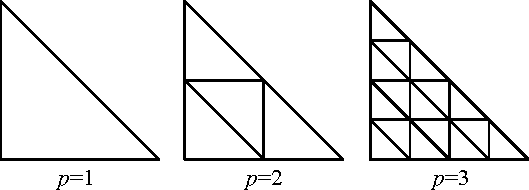
\includegraphics[width=8cm]{Refinement}
\caption{Homogeneous refinement for higher-order finite elements solution visualization.}
\label{fig:Refinement}
\end{figure}

\section{Numerical tests}

This section presents the analysis of four different 3D microwave problems analyzed by FES-3D with the respective comparisons with HFSS (version 10) models:
\begin{itemize}
\item a millimeter-wave E-plane bandpass filter \cite{bui1984broad},
\item a Ka-band corrugated circular horn tailored for radio-astronomy \cite{lucci2005corrugated}, 
%\item a 2.4 GHz, single feed circular polarization patch antenna \cite{maddio2011new},
\item a simple perfect electric scattering sphere.
\end{itemize}

The purpose these tests is to validate the capabilities of the formulations implemented and show some of the features of FES. The core of FES will be extended in the next chapters, where a domain decomposition methods and harmonic balance for nonlinear analyzes of microwave devices will be presented. Current computations are made on AMD Phenom II X4 965 processor with 16 GB of available DDR3 physical memory.

\subsection{Millimeter-wave E-plane bandpass filter analysis}

\begin{figure}[ht!]
\centering
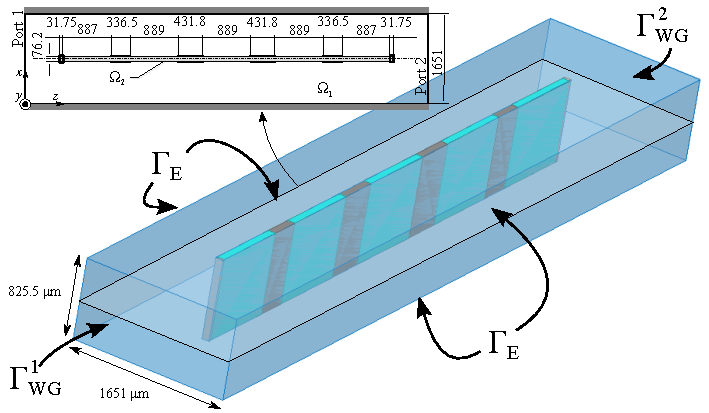
\includegraphics[width=13.4cm]{Bui1984}
\caption{Sketch for the millimeter-wave waveguide filter analyzed and its cross section (H-plane). Measures are given in $\mu m$. }
\label{fig:Bui1984}
\end{figure}

The passband filter designed and presented in \cite{bui1984broad} is realized
by placing on the E-plane a dielectric slab ($\epsilon_r = 2.1$ in $\Omega_2$) partially metalized on both sides in a WR6 rectangular waveguide (Fig. \ref{fig:Bui1984}). All metallic parts will be considered in the FE model as perfect electric conductor. The remaining of the device is devoid of air.

The mesh is composed of 9,686 tetrahedra (not visible here) for a total of 2,074 conjunction nodes. The mesh assembly, with second order basis functions, required about 1.3~s for each frequency of analysis. The boundary conditions where then imposed on the waveports considering both the formulations presented in the previous section. Each 2D eigenmode problem, with second order basis functions, could be solved in approximately 0.4~s. The ARPACK solver, using MUMPS for matrices inversion in the $\mat{B}$-orthogonalization, converged in only 19 iterations (to $10^{-12}$). The dominant mode formulation lead to 57,524 unknowns for a full second order assembly while the transfinite element required less, 56,490 unknowns, as the unknowns on the waveports where removed from the system matrix. 
The overall assembly and solve times where, with the single precision solver, about 5.5~s (2.3~s + 3.2~s) and requiring 132~MB of memory. The double precision solver required approximately the same times, while about twice the memory (255~MB) was needed. Notice that HFSS required only 2~s and about 130~MB of memory for this problem. This could be imparted mainly to the fact it employs a mixed precision solver \cite{sun2008high} for real matrices (in fact they are as no material losses or absorbing boundary conditions are introduced). This kind of solvers iteratively refines the solution provided by a single precision solver $\vect{x}_\mathrm{s}^i =\mat{A}_\mathrm{s}^{-1}\vect{b}_\mathrm{s} \rightarrow \vect{x}_\mathrm{d}^i$ , upon computing a double precision residual vector $\vect{r}_\mathrm{d} = \vect{b}_\mathrm{d} - \mat{A}_\mathrm{d}\vect{x}_\mathrm{d}^i$. Then, the problem on the residual ($\vect{r}_\mathrm{d} \rightarrow \vect{r}_\mathrm{s}$) is solved and added to the double precision solver: $\vect{x}_\mathrm{d}^{i+1} \leftarrow \vect{x}_\mathrm{d}^i + \mat{A}_\mathrm{s}^{-1}\vect{r}_\mathrm{s}$. $s$ and $d$ subscripts correspond, respectively, to single and double precision versions of the matrices or vectors. Furthermore, the use of real matrices noticeably reduce the computational requirements. However, as the purpose of the implemented package is to introduce new computational methodologies, for instance domain decomposition and nonlinear analyzes, the use of real solvers (available with MUMPS) has not been implemented yet.

\begin{figure}[ht!]
\centering
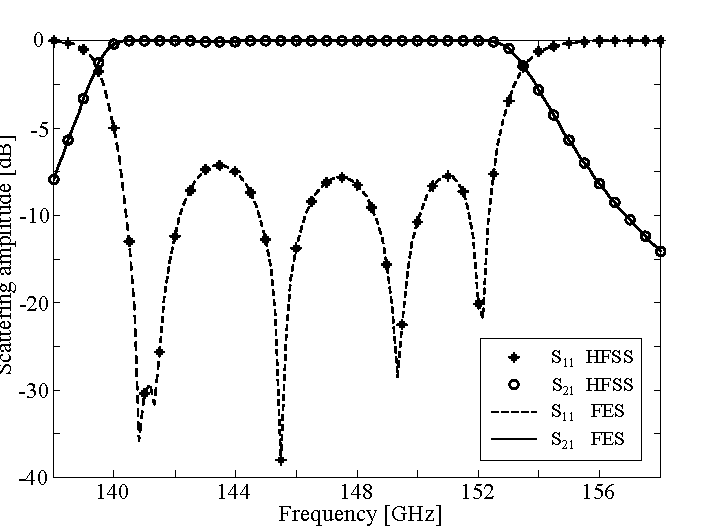
\includegraphics[width=10cm]{Bilat3Dresponse}
\caption{Frequency response of the dominant $\mathrm{TE}_{10}$ mode in the filter, computed with single precision MUMPS solver and dominant mode waveports boundary condition.}
\label{fig:Bilat3Dresponse}
\end{figure}

The frequency (linear) response of the filter, computed with the single precision solver with dominant mode boundary condition on ports, visibly results to be in good agreement with HFSS. In fact, as single precision solver has a numerical error floor of $\approx 10^{-6}$, the dynamic response of the device ($\approx -40~\mathrm{dB} ~\mathrm{to}~0~\mathrm{dB}$) could fit in the dynamic range of numerical precision.

\begin{table}[h!]
\begin{center}
\begin{tabular}{|c|c|c|c|}
\hline 
Dominant (s) & Dominant (d) & Transfinite (s) & Transfinite (d) \\ 
\hline
\hline
$   1.5351 \ 10^{-6}$ & $1.3643 \ 10^{-6}$ & $5.6383 \ 10^{-7}$ & $1.6853 \ 10^{-12}$ \\ 
\hline 
\end{tabular}
\end{center}
\caption{Comparison between the average Euclidean errors for both waveport continuity formulations (only dominant $\mathrm{TE}_{10}$ mode retained), varying the solver precision (s=single, d=double).}
\label{tab:Bilatprecision}
\end{table}

Table \ref{tab:Bilatprecision} shows the relative error $\mathcal{L}^2\left(\mat{S(f)}, \ f\in [138,158]~\mathrm{GHz}\right)$ between the four combinations of waveports formulations and solvers precisions and the solution provided by the mixed precision (real) solver of HFSS in discrete sweep mode. The error is averaged on the 41 equally spaced selected frequency points within the range specified. As we can see, the lower accuracy of the dominant mode formulation is such that a double precision solver does not improve computations. Nevertheless, there no practically appreciable differences between the responses (Fig. \ref{fig:Bilat3Dresponse}). The transfinite element formulation, being more robust, is such that equivalence in results is achieved within numerical precision.


\begin{figure}[h!]
\centering
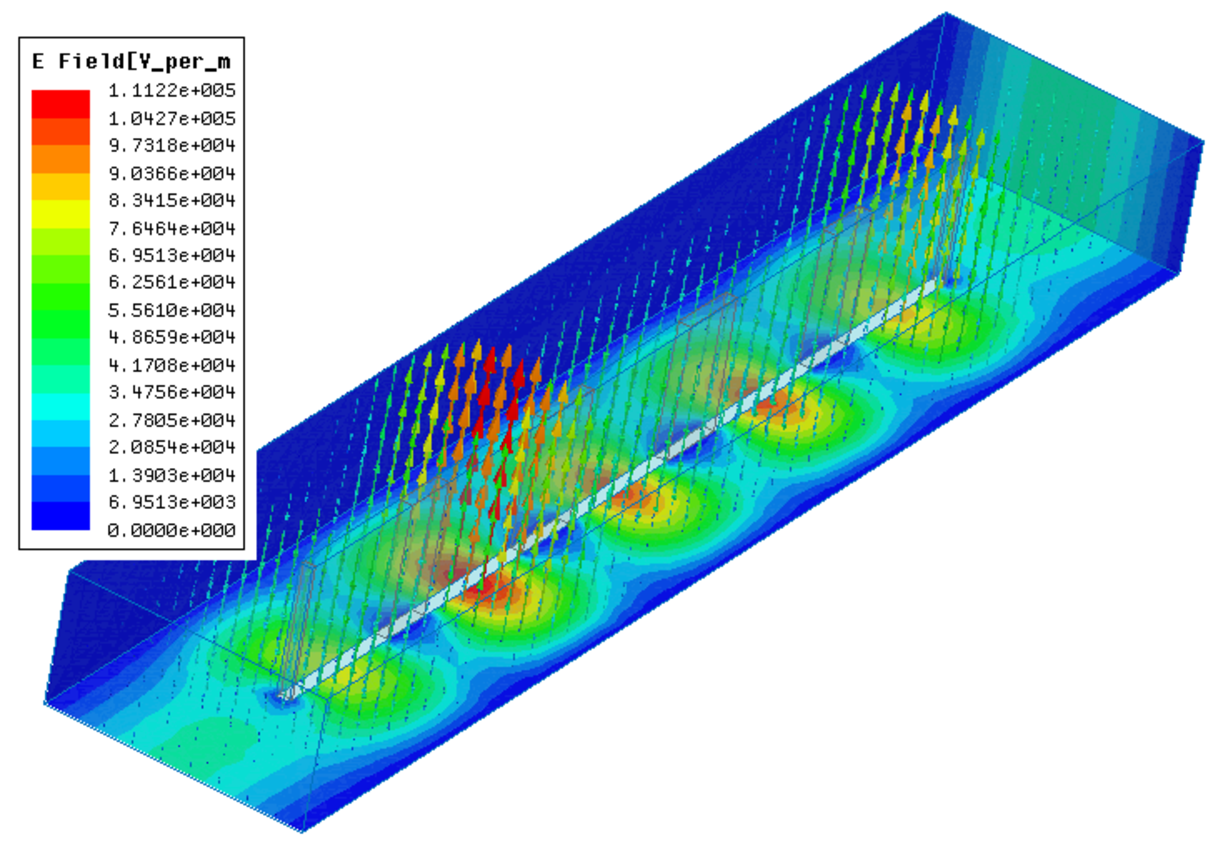
\includegraphics[width=13.4cm]{Bilat3DHFSS}
\caption{Electric field at 150 GHz computed by means of HFSS.}
\label{fig:Bilat3DHFSS}
\end{figure}

\begin{figure}[h!]
\centering
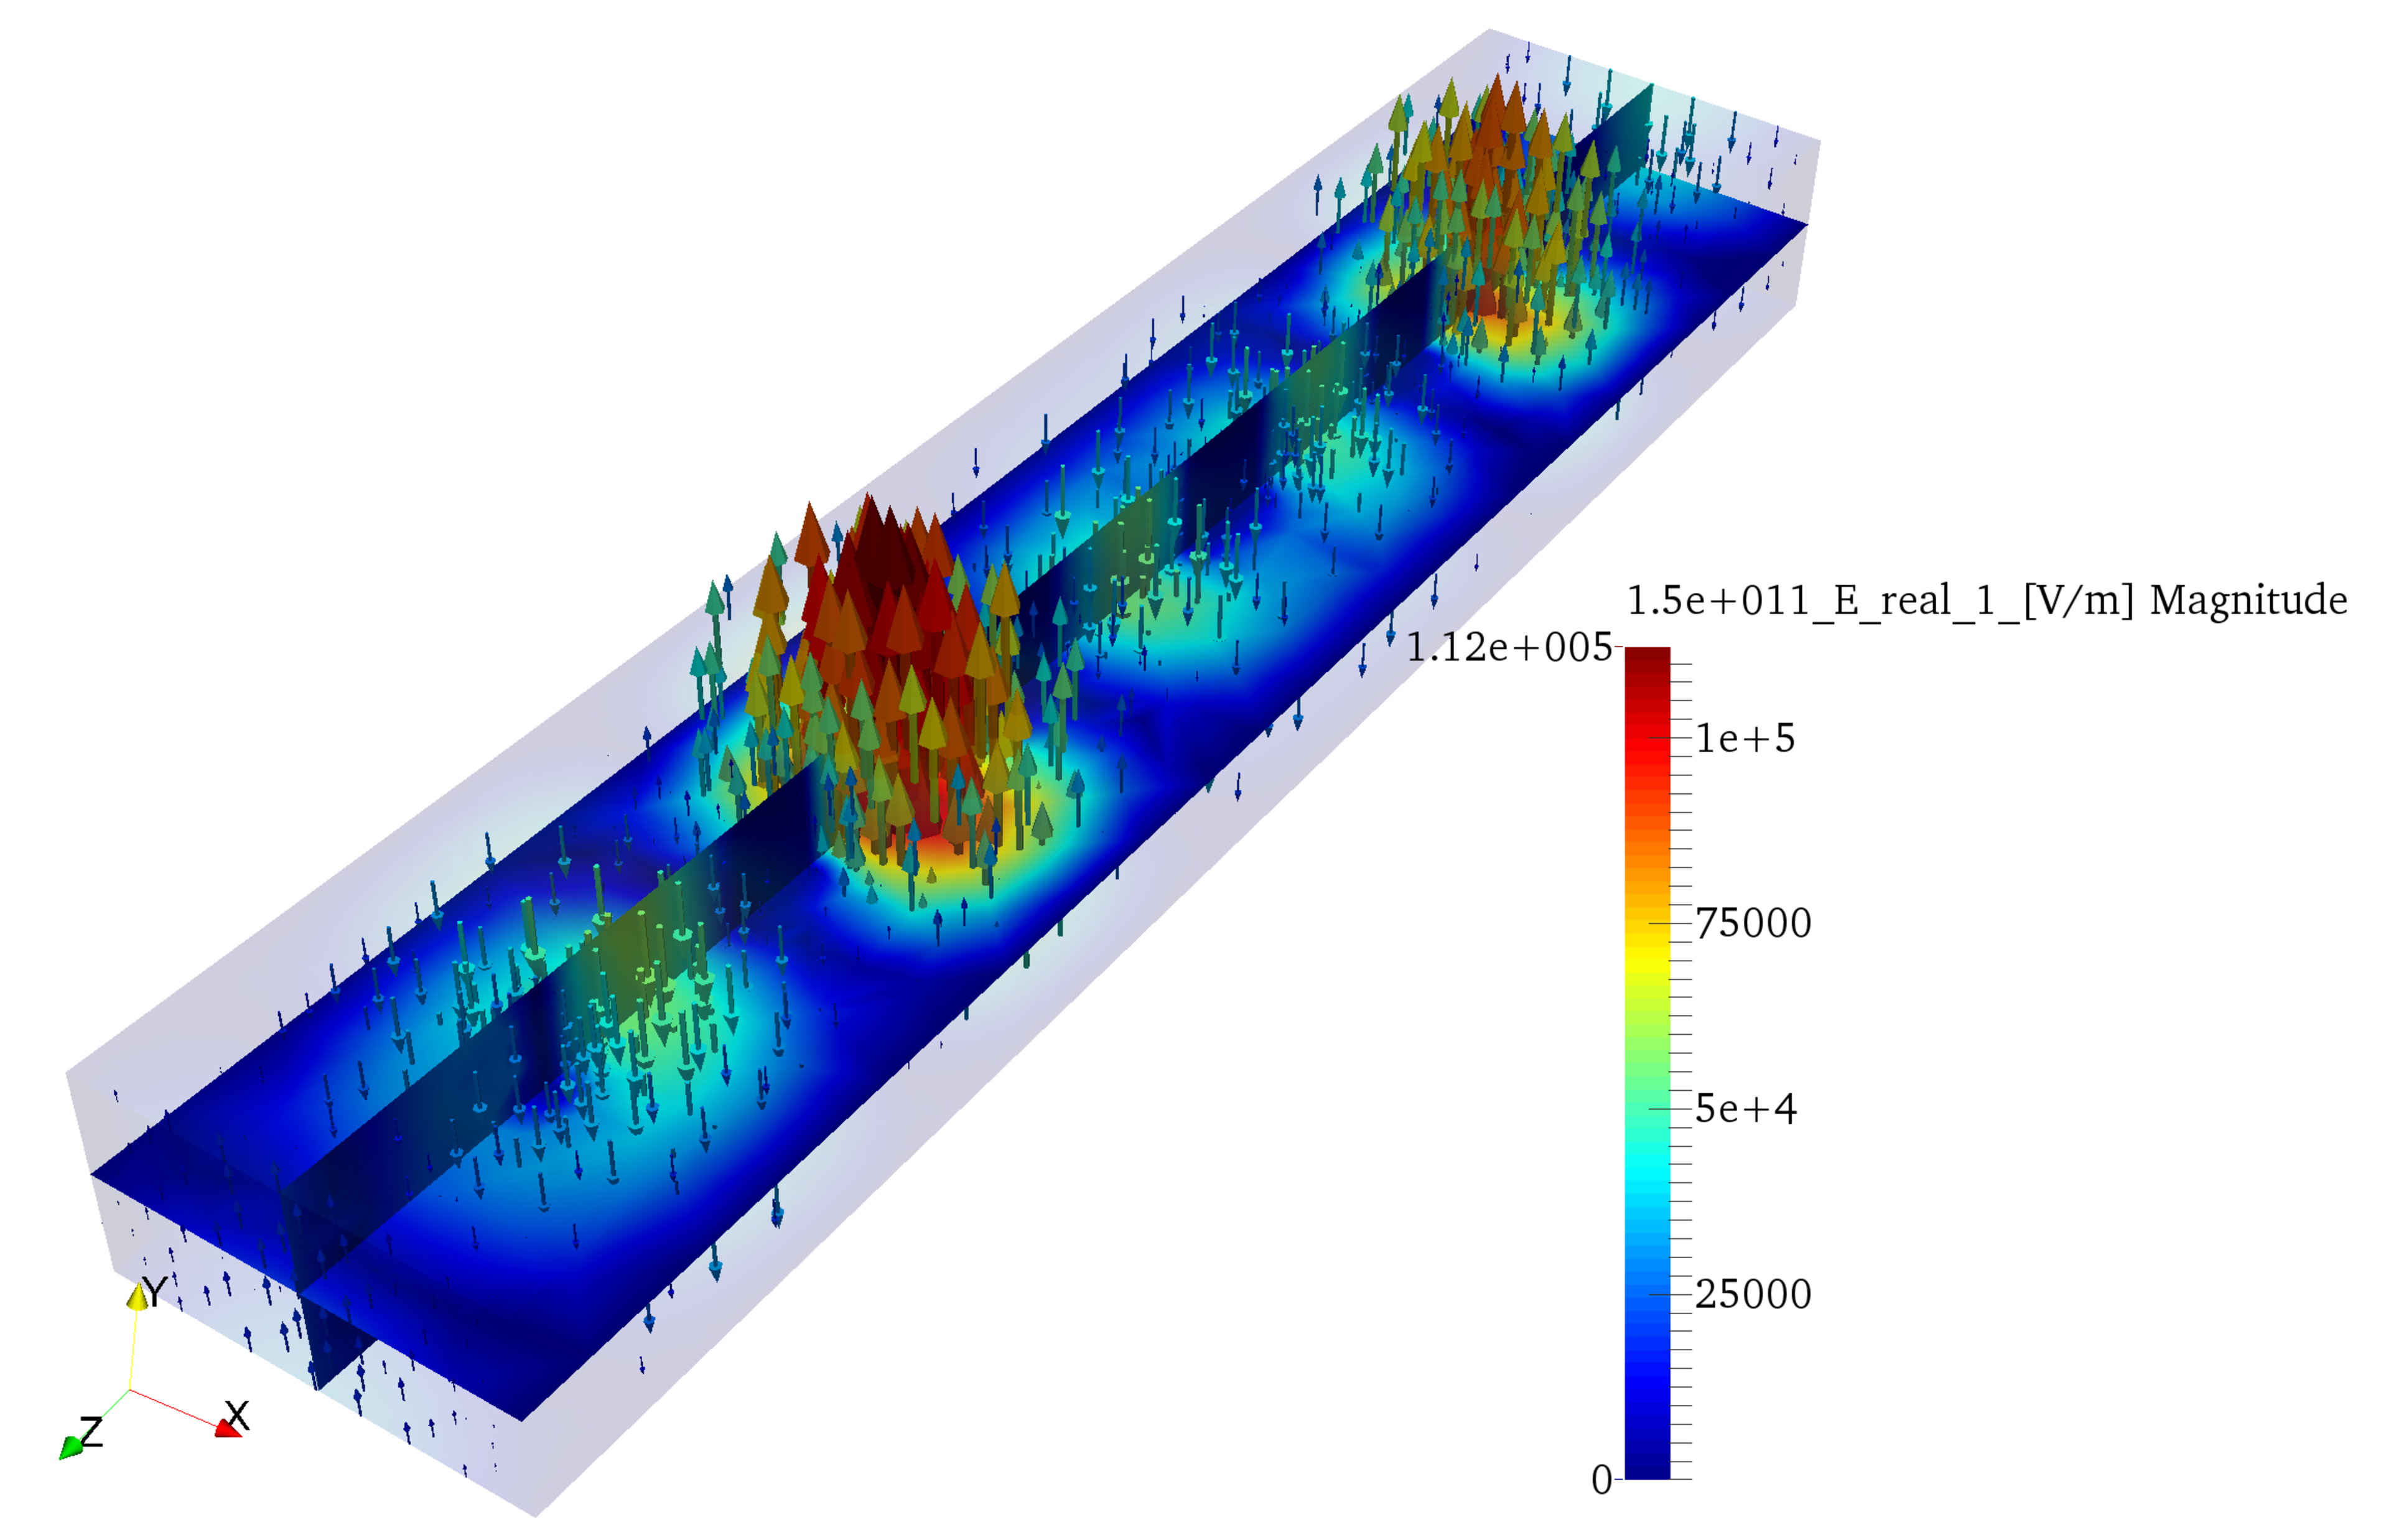
\includegraphics[width=13.4cm]{Bilat3D}
\caption{Electric field at 150 GHz computed by means of FES and visualized in Paraview.}
\label{fig:Bilat3D}
\end{figure}

After the computation of scattering parameters, one might be interested in visualizing the fields at a given frequency. Figs. \ref{fig:Bilat3DHFSS} and \ref{fig:Bilat3D} show the electric fields (real parts) computed at 150~GHz. The electric and magnetic fields, in FES, are computed upon interpolating the respective shape functions at the nodes of the mesh (refined in this case as $p=2$). There is a good agreement between the two electromagnetic solvers and maximum amplitude of the electric field of $\approx 112~\frac{\mathrm{kV}}{\mathrm{m}}$ is attained within the device. Vertical and horizontal cut-planes can be easily obtained in Paraview upon selecting the \quotes{slicing} function. 

\subsection{Corrugated circular horn analysis} \label{sec:Horn}

\begin{figure}[ht!]
\centering
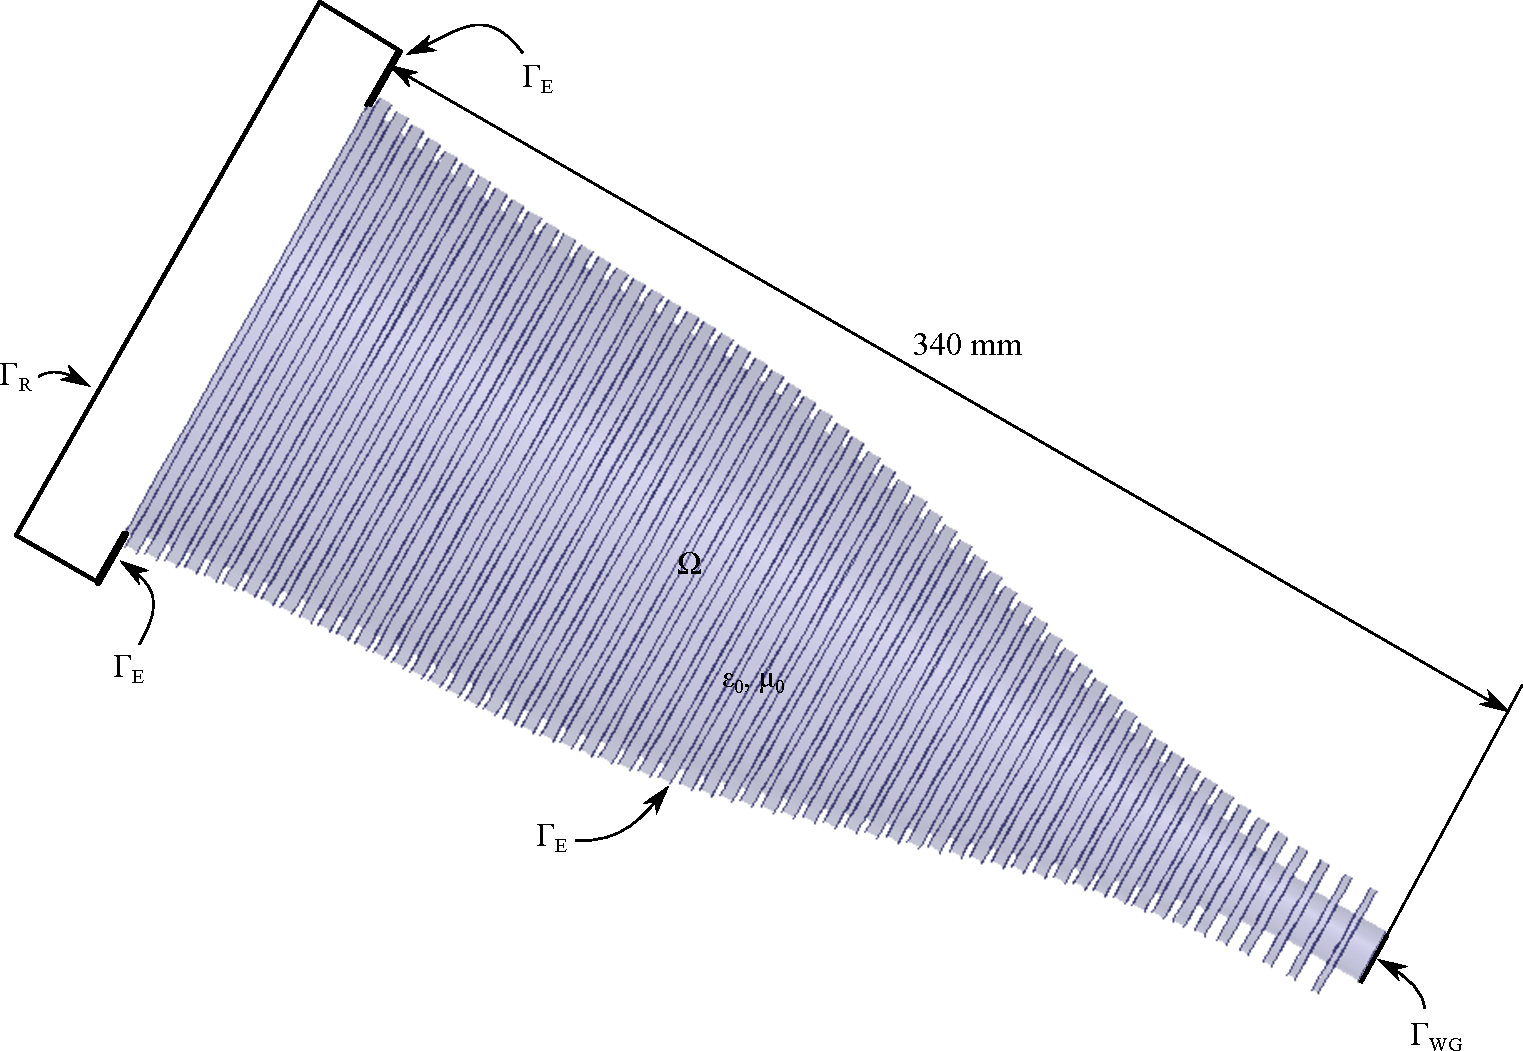
\includegraphics[width=13.4cm]{CircHornSketch}
\caption{Sketch of the 22 GHz corrugated circular horn antenna.}
\label{fig:CircHornSketch}
\end{figure}

In the work \cite{lucci2005corrugated}, there were shown a 22~GHz corrugated circular horn antenna built at the \quotes{Osservatorio Astrofisico di Arcetri}, an institute for radio-astronomical studies of the (Italian) National Research Council. That horn,  whose model is depicted in Fig. \ref{fig:CircHornSketch}, is made of 60 corrugations in order to smooth gradually the transition between guided waves to radiated waves and achieve a pure linear polarization. This procedure results in a better tapering of the radiation pattern, significantly lowering the side lobes. In its designed working conditions, the horn is fed with two degenerate $\mathrm{TE}_{11}$ circular waveguide modes in quadrature: they are both physically oriented perpendicularly and with 90\textdegree~of phase shift.

Here, we have tested the capabilities of FES to analyze multimode problems, with the transfinite element method, and it is a first attempt to evaluate radiation boundary conditions. Notice that antenna is about 25 wavelengths long and the corrugations dramatically increase tetrahedra's number of the mesh, for conformity constraints to the geometry.  The antenna is terminated at its narrower end by a circular waveport boundary and at the mouth or aperture of the horn, by a parallelepiped box on which radiation conditions are imposed. Of course, both horn and box are merged in order to have a unique enclosed medium devoid of air. Simulations are performed with cubic order shape functions.

\begin{figure}[ht!]
\centering
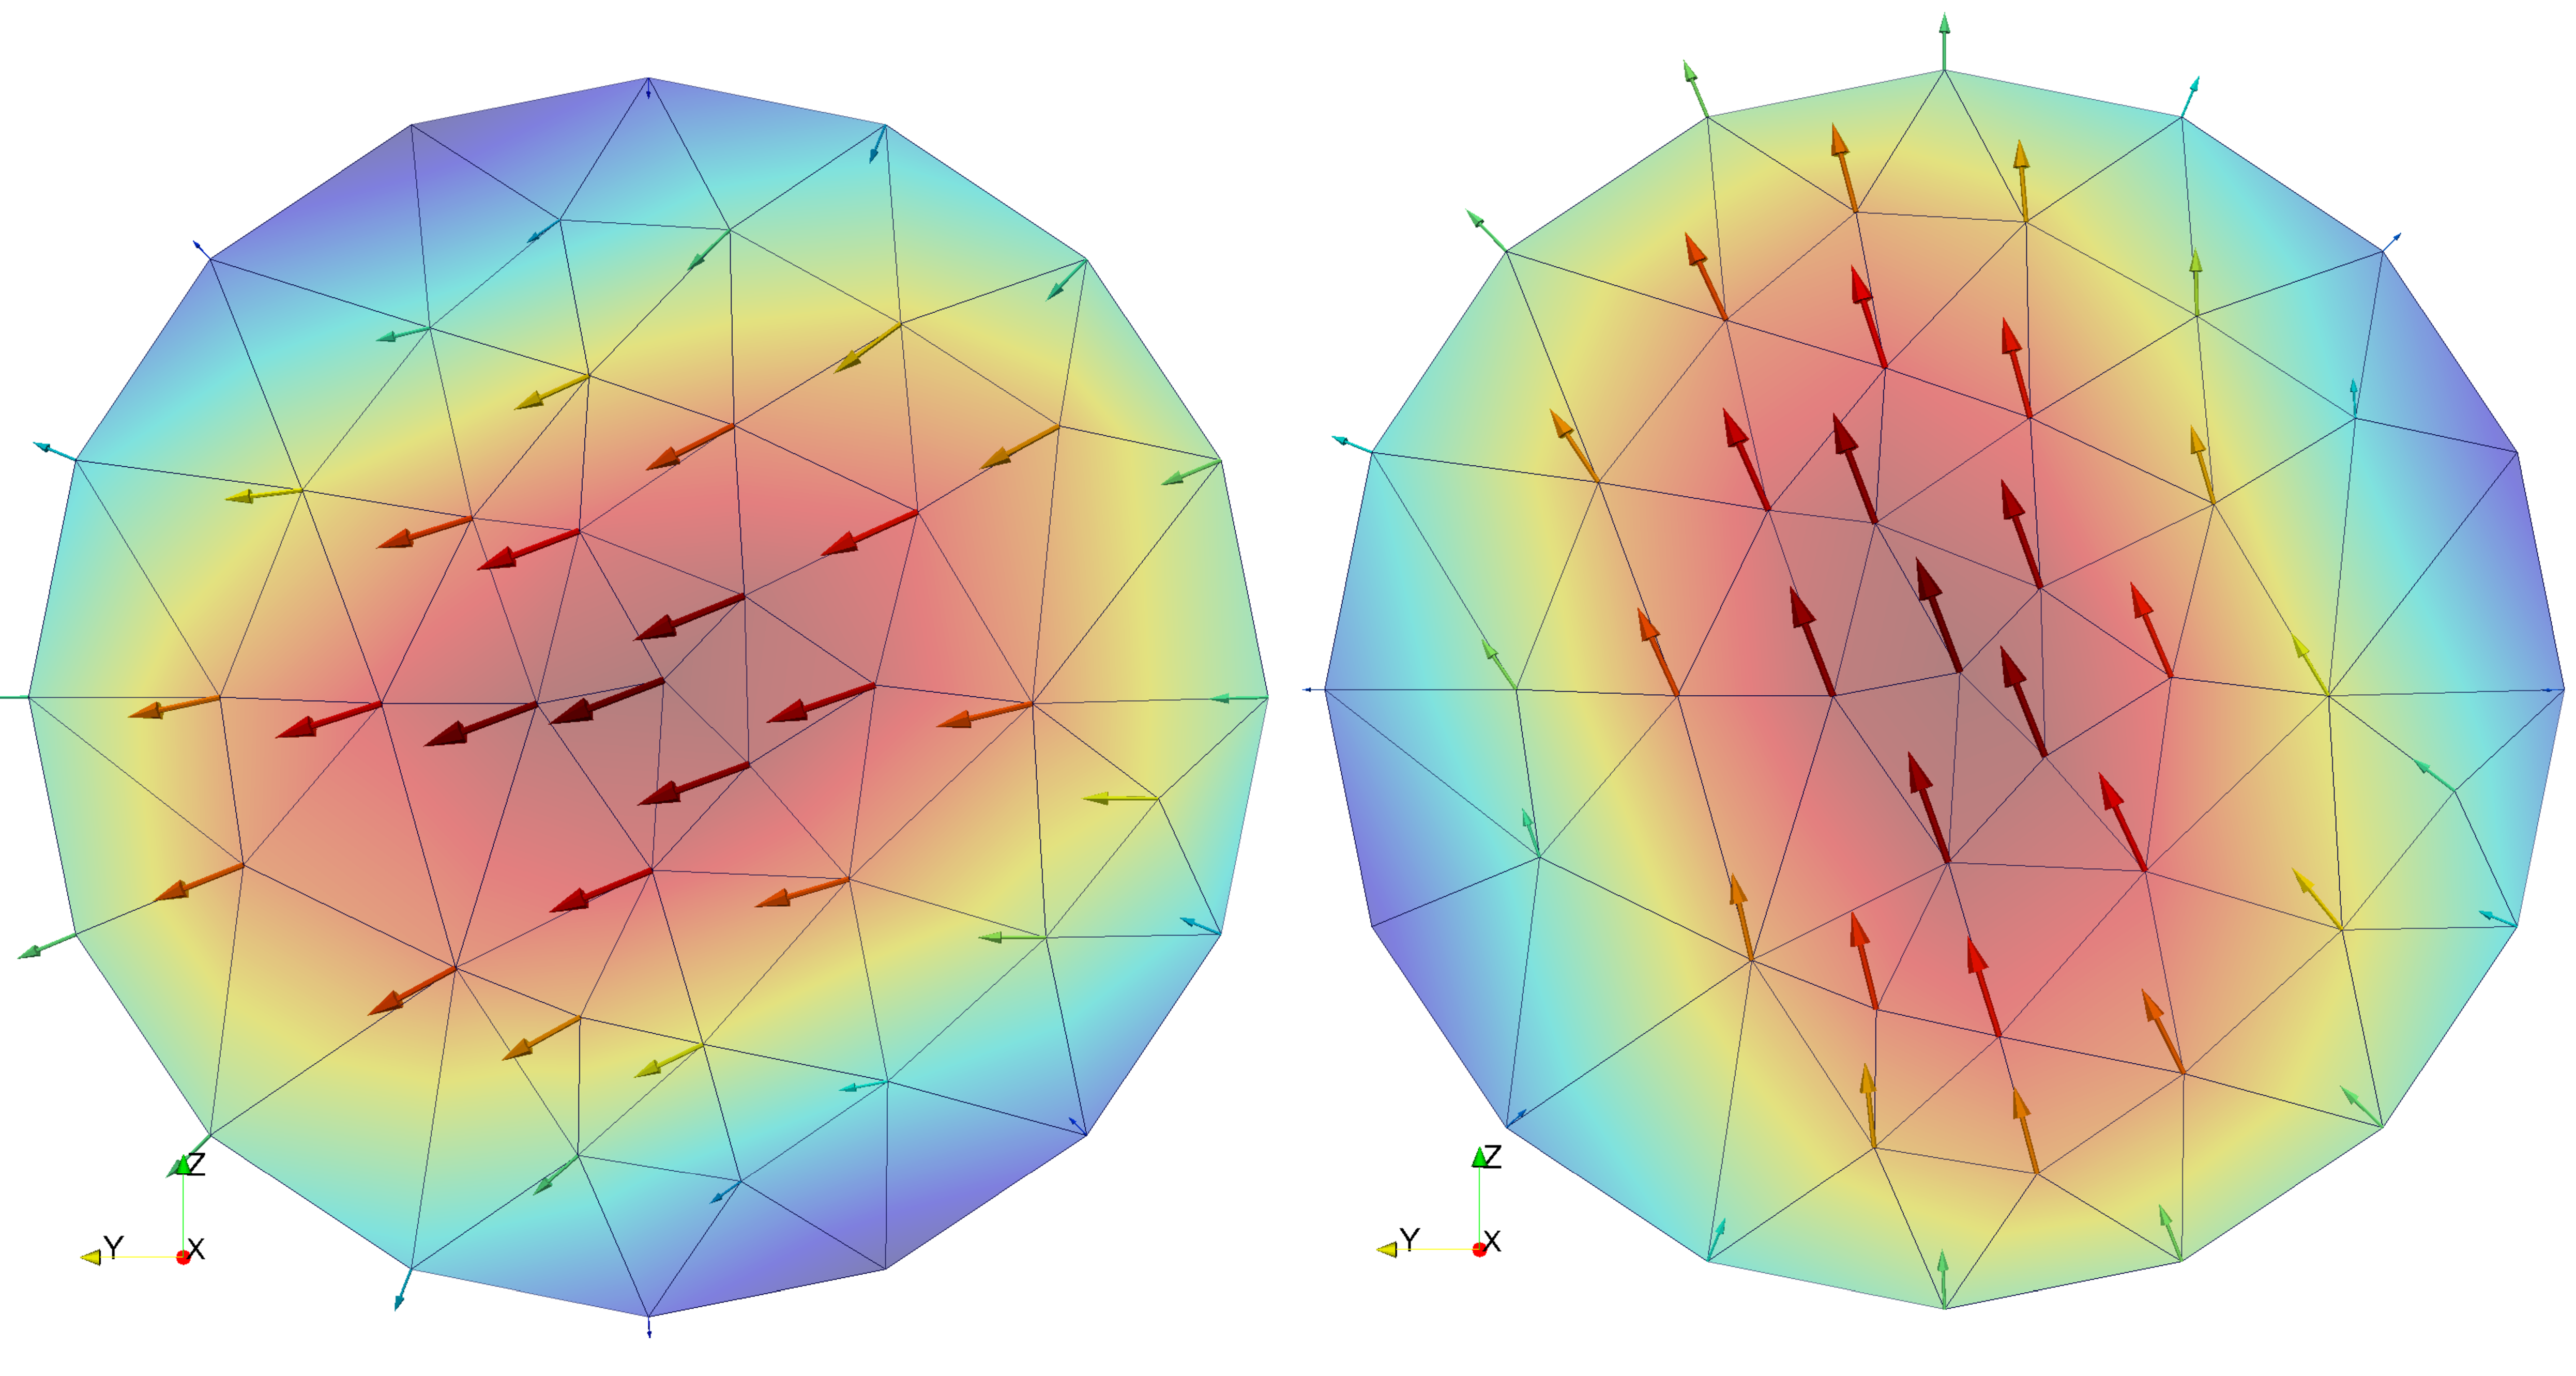
\includegraphics[width=8cm]{Modes}
\caption{Degenerate $\mathrm{TE}_{11}$ modes feeding the antenna (in quadrature).}
\label{fig:Modes}
\end{figure}


The first five modes were computed with ARPACK, and 36 iterations where needed to converge in about 2~s. The excitation modes are shown Fig. \ref{fig:Modes}. Then the assembly and solve on 602,594 unknowns (36,331 tetrahedra) required for the single precision solver about 123~s while the double precision 170~s. In fact, as both the matrices are assembled in the double precision, the single precision solver required 47~s less than its double precision counterpart. Also, memory requirements where different: 3,158~MB for the single precision and 6,159~MB for the double. Notice that HFSS required 146~s and 3.7~GB of memory to solve the problem with its mixed precision complex solver, which is in good agreement with what was stated before.

\begin{eqnarray*}
|\mat{S}|_\mathrm{dB}^\mathrm{HFSS} & = &
\begin{bmatrix}
  -49.7001 & -60.5669 & -55.9466 & -82.8433 & -79.8956 \\
  -60.5669 & -49.9378 & -46.5148 & -87.5034 & -81.1233 \\
  -55.9460 & -46.5148 &  -3.4413 & -80.8478 & -86.5927 \\
  -82.8433 & -87.5033 & -80.8478 & -48.4840 & -88.2707 \\
  -79.8958 & -81.1234 & -86.5927 & -88.2707 & -48.3815
\end{bmatrix},\\
|\mat{S}|_\mathrm{dB}^\mathrm{TFE,single} & = &
\begin{bmatrix}
  -49.0035 & -63.4025 & -64.6486 & -80.1454 & -80.7432 \\
  -63.2030 & -49.6485 & -46.1201 & -91.9744 & -82.0608 \\
  -64.4864 & -46.1409 &  -3.4416 & -81.8164 & -84.3125 \\
  -80.1613 & -91.9789 & -81.8047 & -48.5274 & -91.8034 \\
  -80.7334 & -82.0586 & -84.3199 & -91.8016 & -48.3397
\end{bmatrix},\\
|\mat{S}|_\mathrm{dB}^\mathrm{TFE,double} & = & 
\begin{bmatrix}
  -49.1332 & -63.1736 & -64.5808 & -80.1579 & -80.7213 \\
  -63.1736 & -49.9021 & -46.1233 & -92.0040 & -82.1035 \\
  -64.5808 & -46.1233 &  -3.4414 & -81.8144 & -84.1136 \\
  -80.1579 & -92.0040 & -81.8144 & -48.5264 & -91.8808 \\
  -80.7213 & -82.1035 & -84.1136 & -91.8808 & -48.3394 \\
\end{bmatrix}.
\end{eqnarray*}

The magnitudes of the scattering parameters, shown above, agree within an average error of $\approx 7 \times 10^{-5}$ for single and double precision FES solvers relatively to HFSS solver. Values are, in practical terms, the same. Differences between the results might be imparted also to the use of different third order shape functions between FES and HFSS.

When analyzing antennas, one might be interested in its performances in terms of directivity or gain. Here, as no lossy materials are present, the gain equals the directivity. Figs. \ref{fig:CircHornRadHFSS} and \ref{fig:CircHornRad} show the radiation solids computed by HFSS and FES (VTK file). The gain of the antenna is of about 25.5~dB, and when fed in quadrature, circular polarization is achieved. The postpocessing time was about 302~s for FES, while only about 51~s for HFSS on 259,200 look angles. In Paraview, it is also possible to visualize the far field $\mathbf{E}(\hat{\mathbf{r}})$ as vectors in order to visualize the polarization achieved (in all directions) while time elapses. Also, slices data can be exported for radiation patterns plots on cut-planes (Fig. \ref{fig:Polar}).

\begin{figure}[h!]
\centering
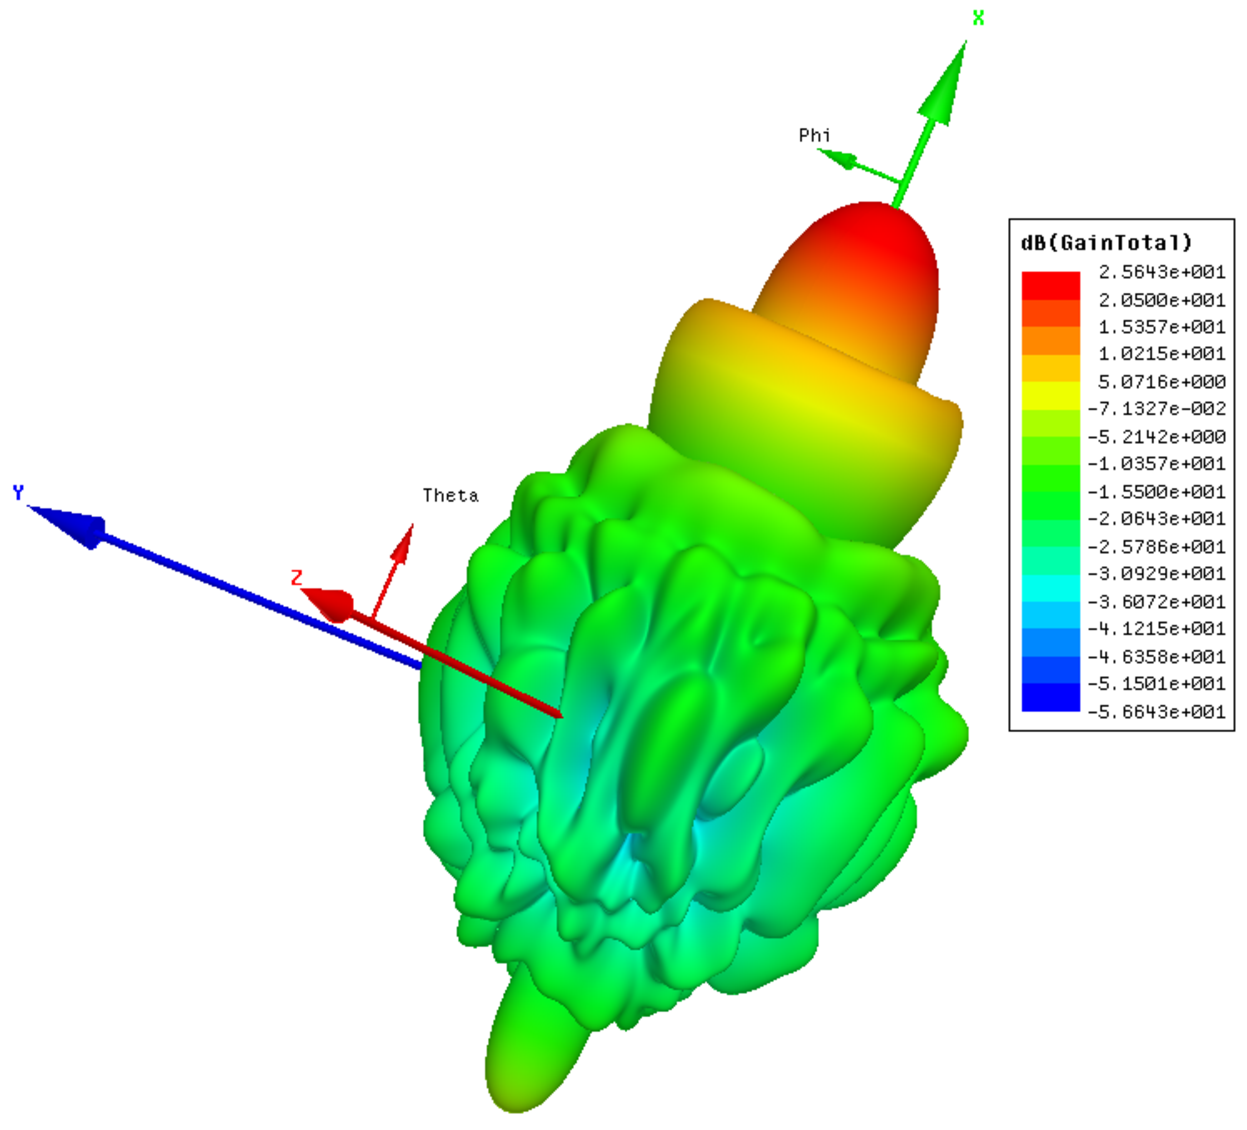
\includegraphics[width=13.4cm]{CircHornRadHFSS}
\caption{Radiation solid at 22~GHz computed with HFSS.}
\label{fig:CircHornRadHFSS}
\end{figure}

\begin{figure}[h!]
\centering
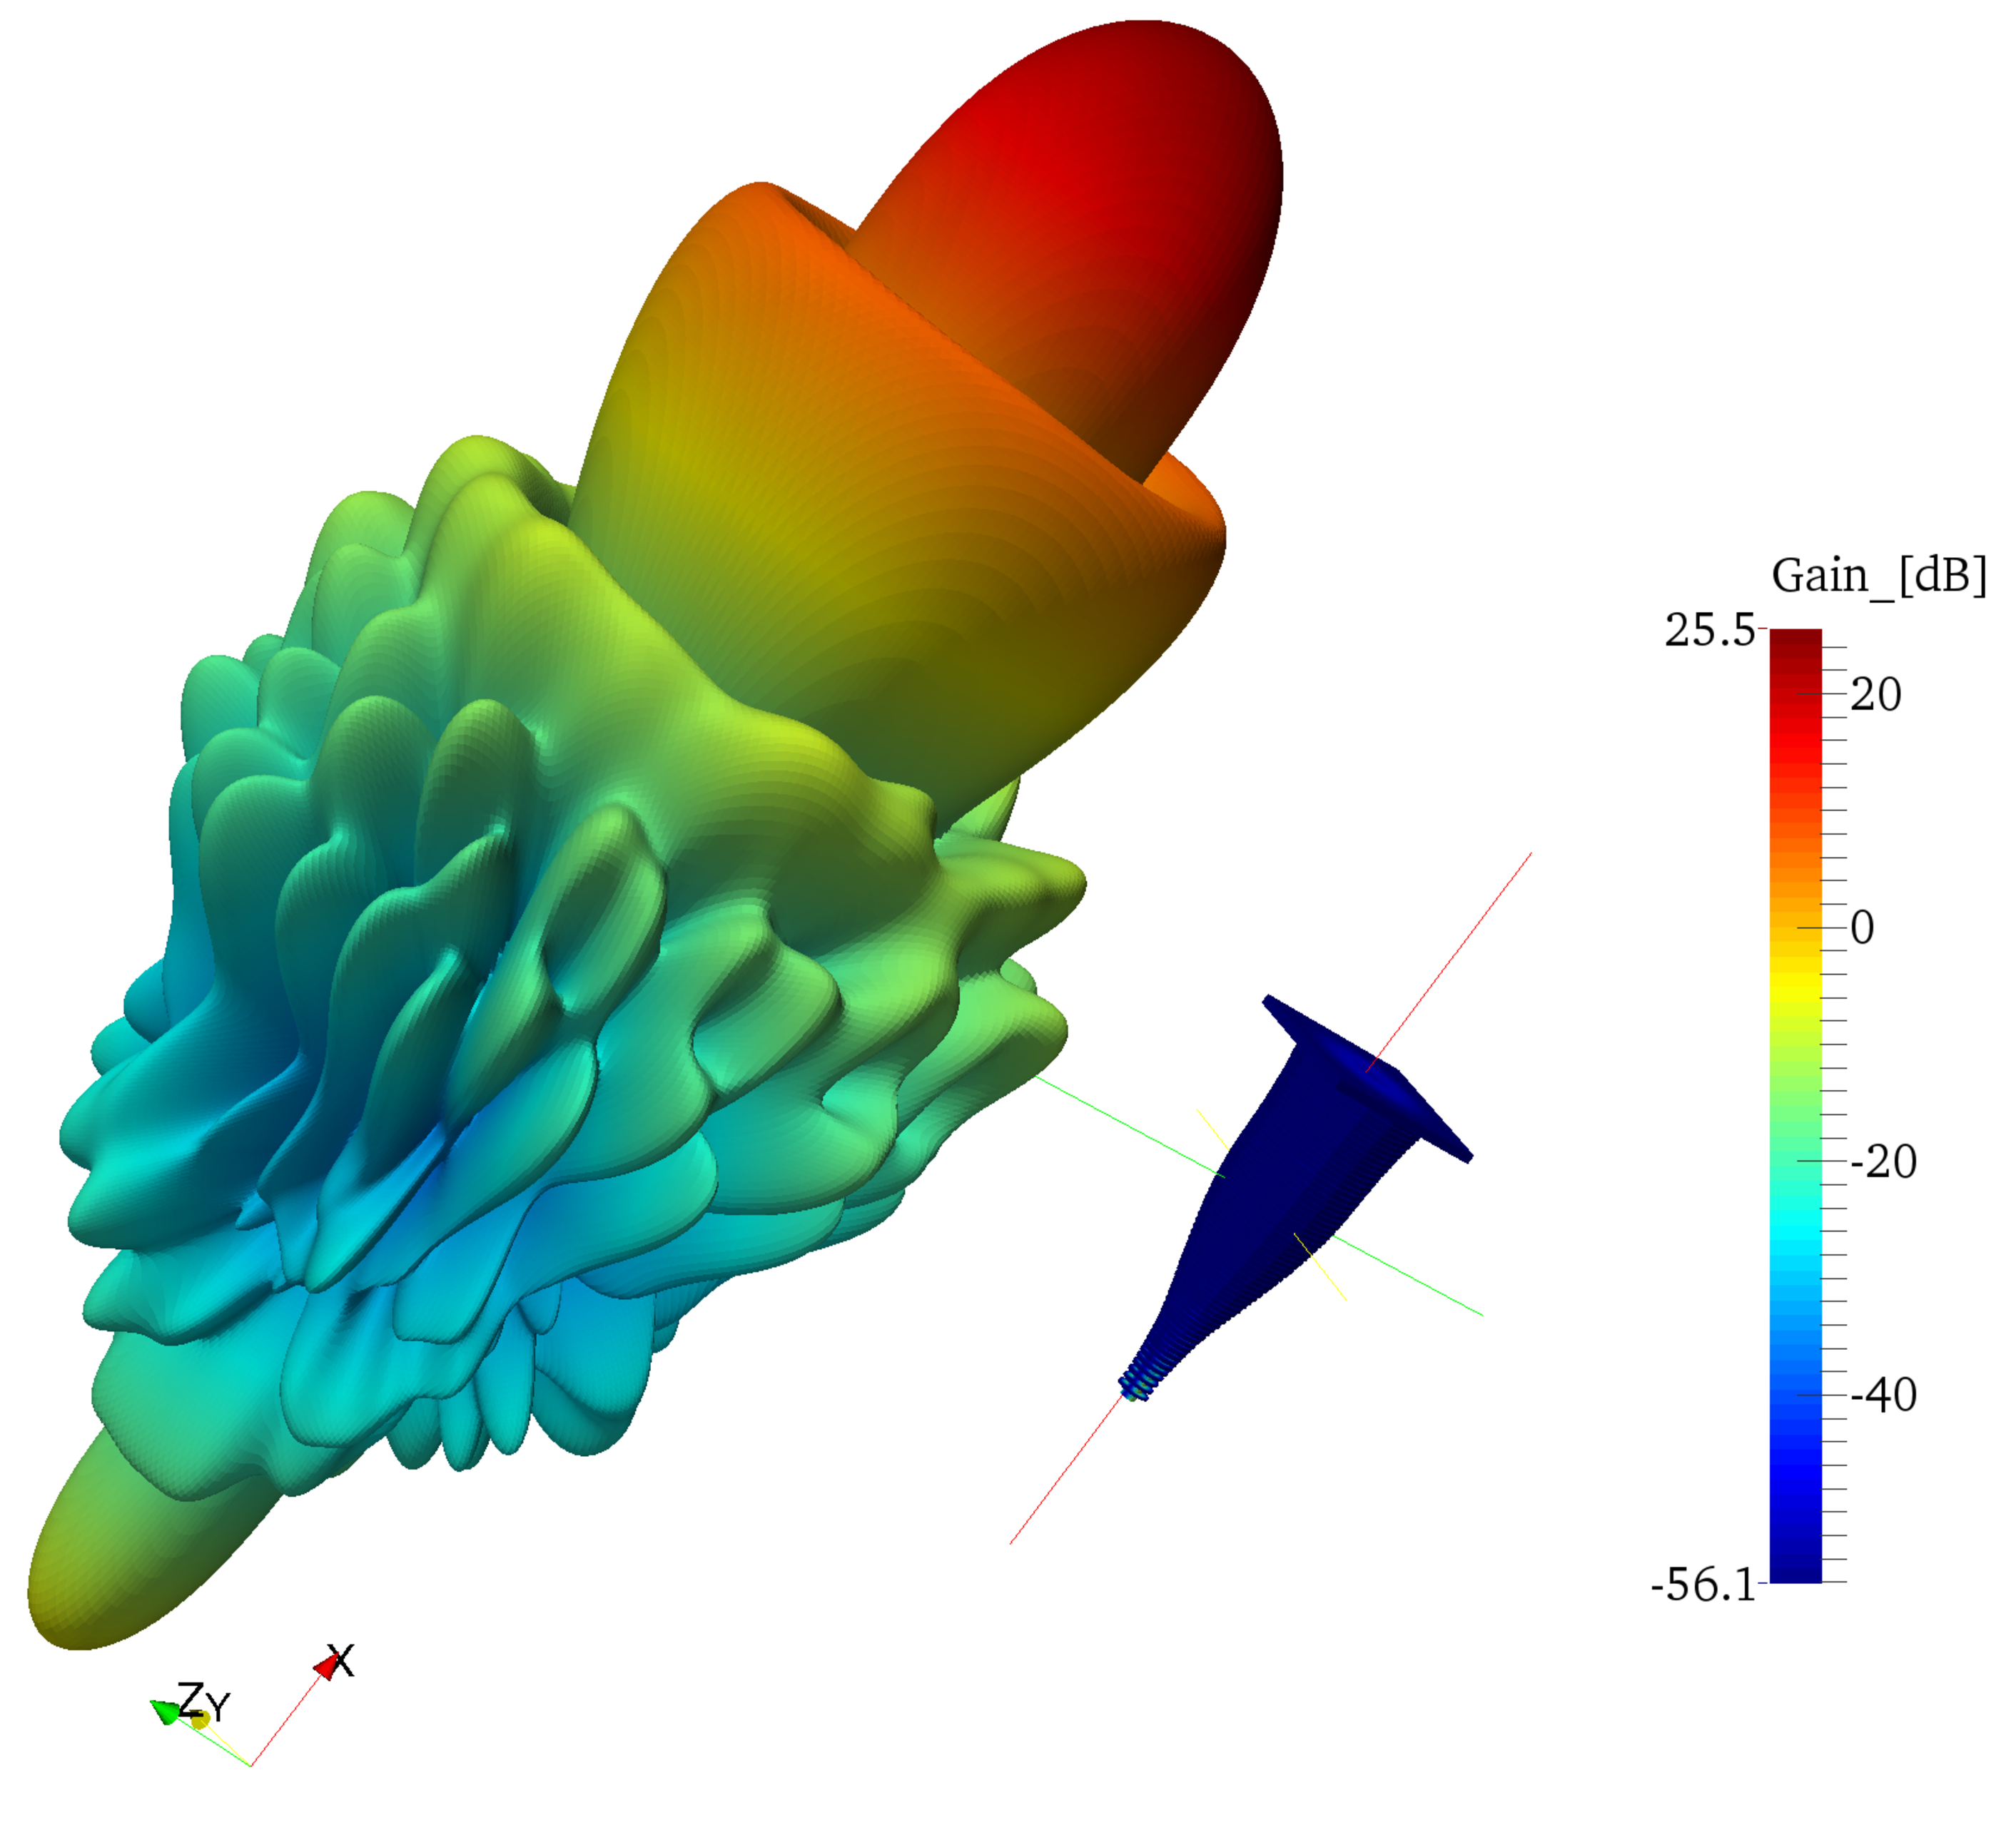
\includegraphics[width=12.4cm]{CircHornRad}
\caption{Radiation solid at 22~GHz computed with FES.}
\label{fig:CircHornRad}
\end{figure}

\begin{figure}[h!]
\centering
\begin{minipage}{6.5cm}
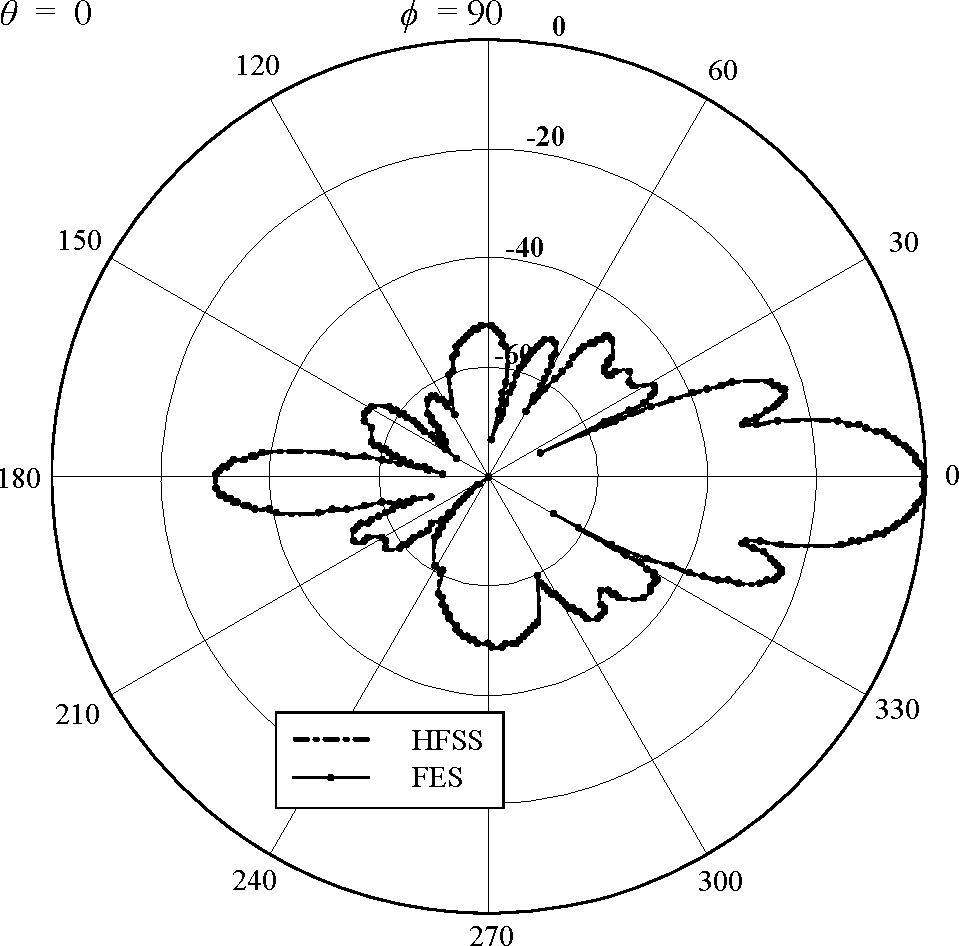
\includegraphics[width=6.4cm]{Polar2}
\end{minipage}
\
\begin{minipage}{6.5cm}
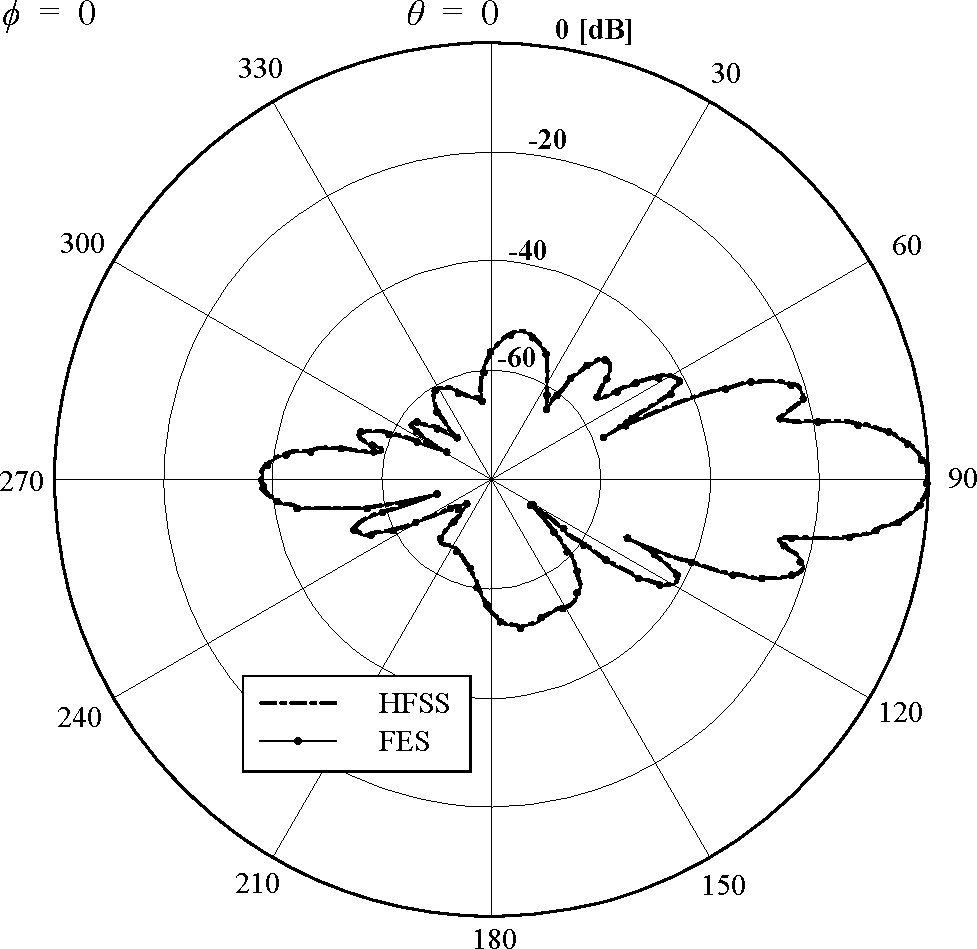
\includegraphics[width=6.4cm]{Polar1}
\end{minipage}
\caption{Normalized gain patterns on the \textit{XY} (left) and the \textit{XZ} (right) planes.}
\label{fig:Polar}
\end{figure}

%\begin{figure}[h!]
%\centering
%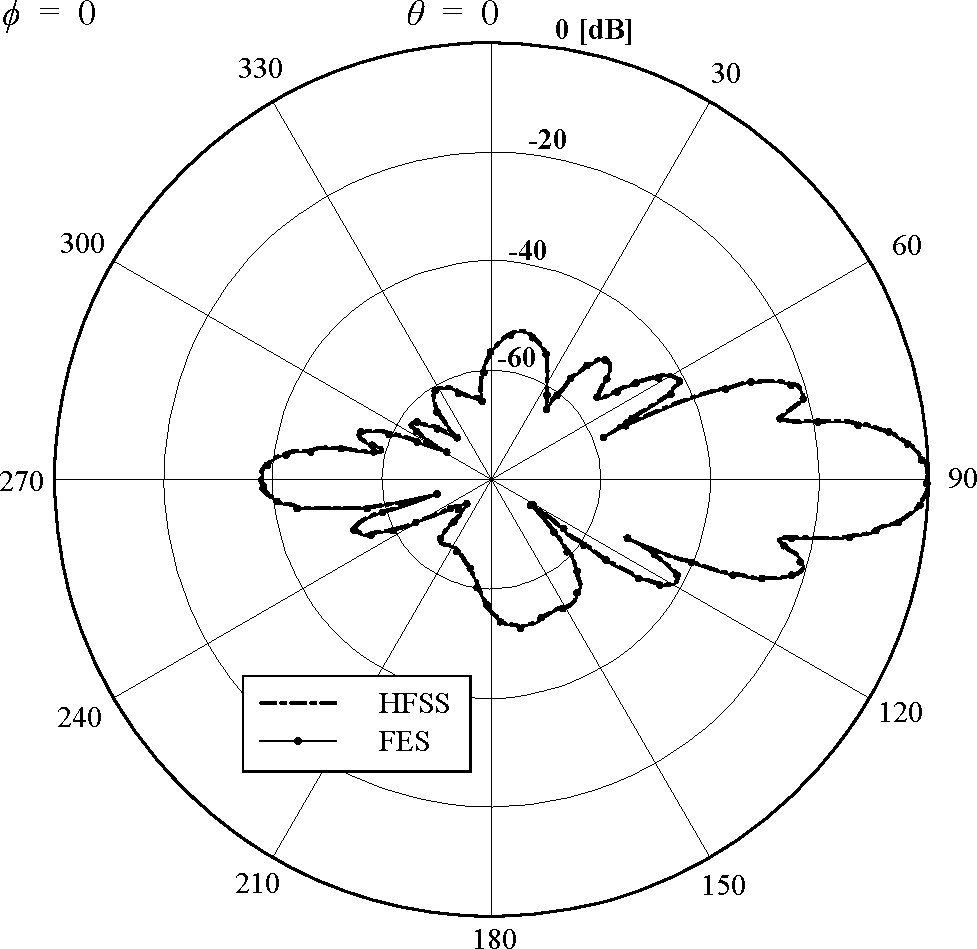
\includegraphics[width=10cm]{Polar1}
%\caption{Normalized gain patterns on the $XZ$ plane comparisons.}
%\label{fig:Polar1}
%\end{figure}


%\subsection{2.4GHz Circular polarization patch antenna analysis}
%
%
%\begin{figure}[ht!]
%\centering
%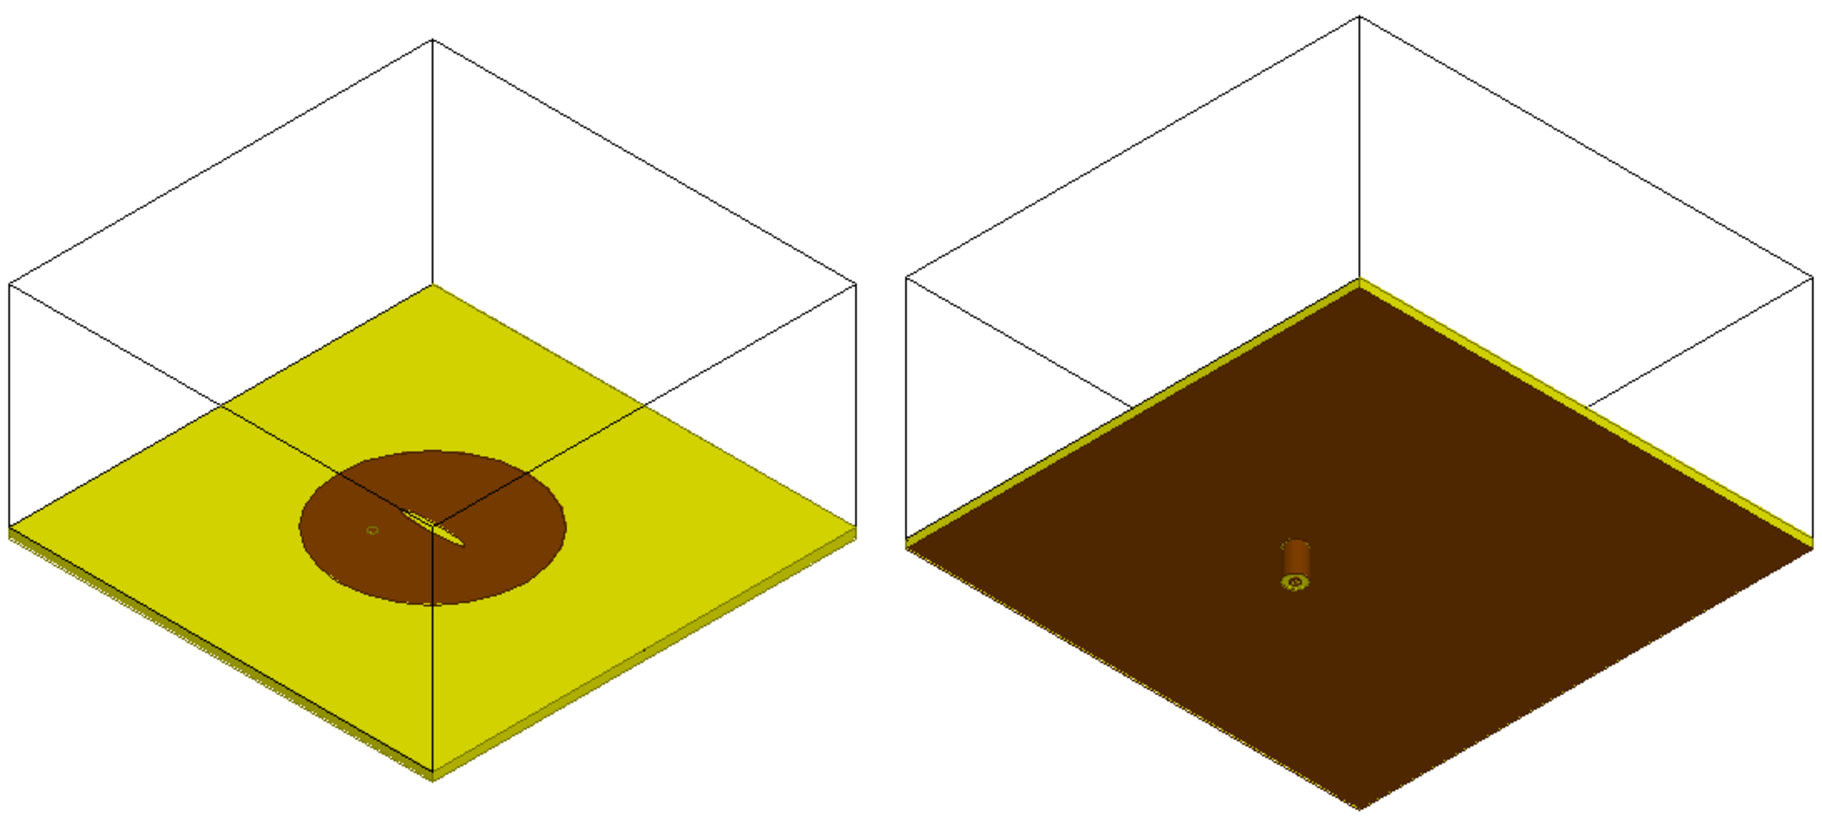
\includegraphics[width=13.4cm]{PatchAntenna}
%\caption{Sketch for the waveguide filter of.}
%\label{fig:PatchAntenna}
%\end{figure}

\clearpage
\subsection{Perfect electric scattering sphere}

Another test, which is \quotes{classical} among all the electromagnetic problems as it founds since more than a century an analytical solution, is that of a metallic sphere located in free-space, made of perfect electric conductor, on which impinges a plane wave from one direction. The domain of finite element analysis is shown in Fig. \ref{fig:Sphere}.

\begin{figure}[ht!]
\centering
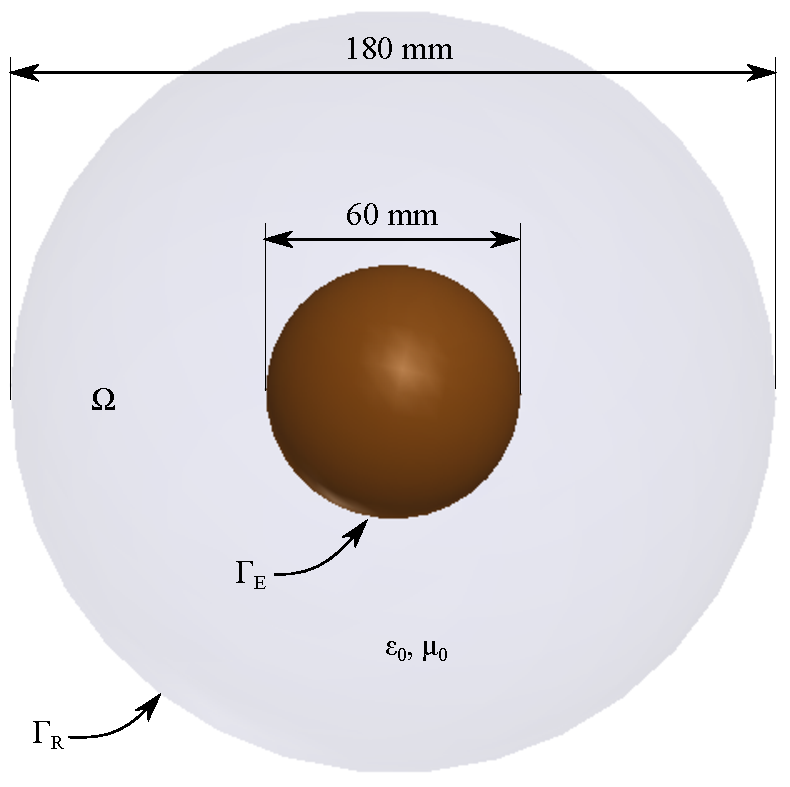
\includegraphics[width=9cm]{Sphere}
\caption{Sketch the scattering problem by a perfectly conducting metallic sphere.}
\label{fig:Sphere}
\end{figure}

Consider a plane wave at frequency $f$, traveling in free-space in the direction $\hat{\mathbf{z}}$. Hence the incident electric field, polarized along $\hat{\mathbf{x}}$, can be written as

$$\mathbf{E}^{inc} = | \mathbf{E}^{inc}| \exp{-jk_0 \hat{\mathbf{z}} \cdot \mathbf{r} } \ \hat{\mathbf{x}},$$

\noindent and the magnetic field

$$\mathbf{H}^{inc} = \frac{1}{\zeta_0} \mathbf{E}^{inc} \times \hat{\mathbf{z}} =  \frac{1}{\zeta_0}| \mathbf{E}^{inc}| \exp{-jk_0 \hat{\mathbf{z}} \cdot \mathbf{r} } \ \hat{\mathbf{y}}.$$

These values can be substituted in the formulation \ref{eq:FEMformScatt} in order to compute the integrals on $\Gamma_R$. In this test case, we have considered the wave, with $| \mathbf{E}^{inc}| = \frac{\mathrm{V}}{\mathrm{m}}$, to be oscillating at 6~GHz. The mesh of 73,252 tetrahedra led to only 89,946 unknowns. The electric fields computed by both HFSS and FES (double precision) are shown in Figs \ref{fig:SphereHFSS} and \ref{fig:SphereField}, considering first order basis functions. The maximum magnitude of the electric field in the domain of analysis $\Omega$ was of about $1.52~\frac{\mathrm{V}}{\mathrm{m}}$ in both cases, and the overall distribution was approximately the same. Due to linear polarization along the $\hat{\mathbf{x}}$ axis, the $XZ$ cut-plane, so-called \textit{E}-plane, shows a different electric field distribution respectively to that on the $YZ$ cut-plane, the \textit{H}-plane.

\begin{figure}[ht!]
\centering
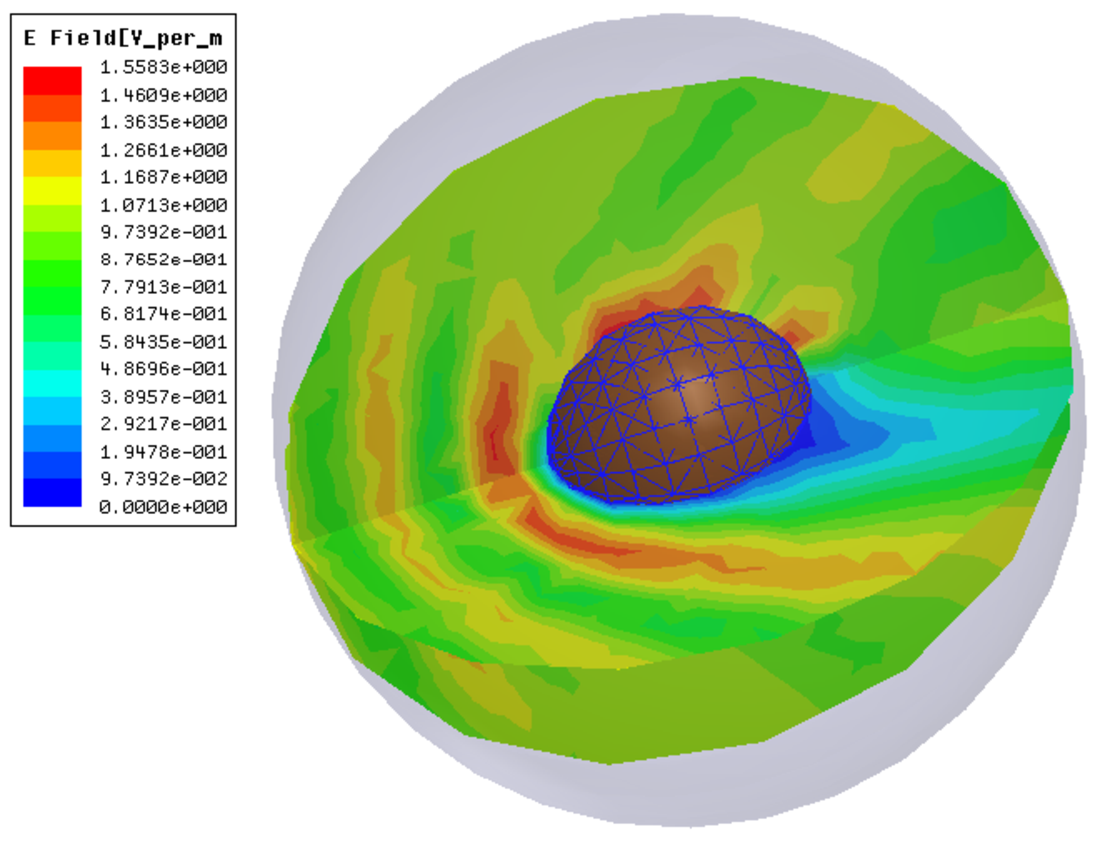
\includegraphics[width=10cm]{SphereHFSS}
\caption{Electric field surrounding the perfectly conducting metallic sphere, computed with HFSS.}
\label{fig:SphereHFSS}
\end{figure}
\begin{figure}[ht!]
\centering
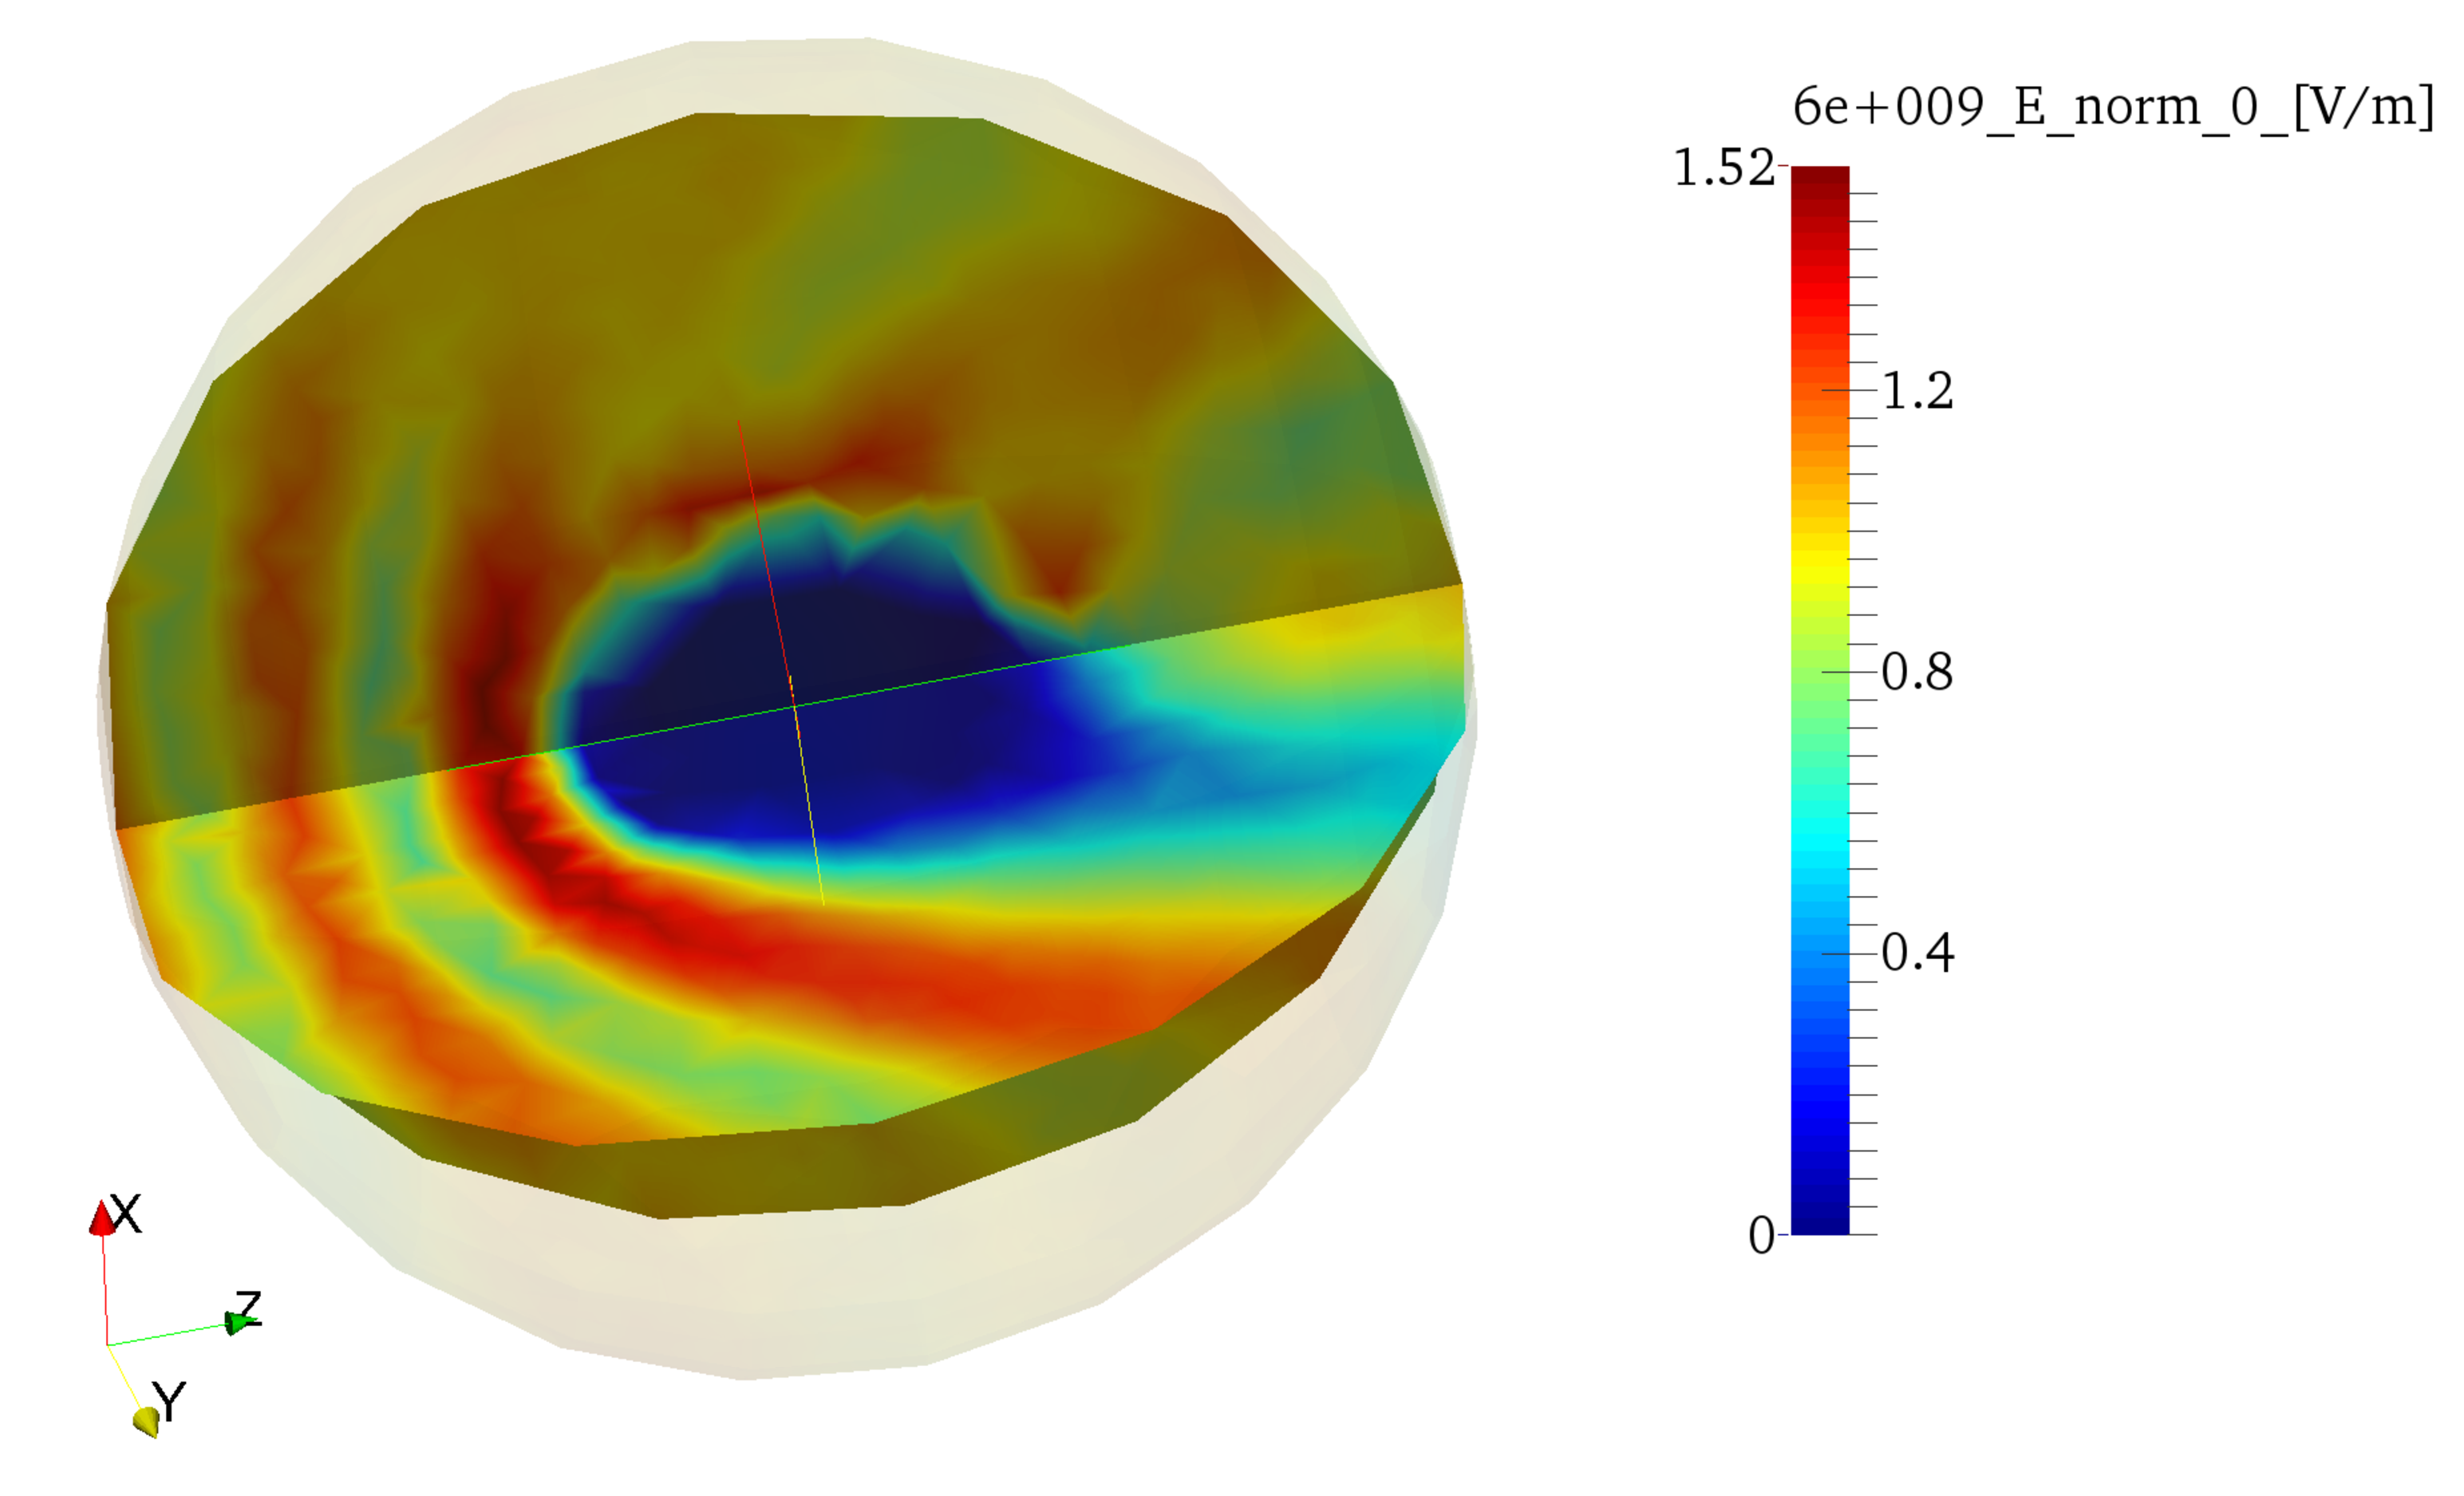
\includegraphics[width=13cm]{SphereField}
\caption{Electric field surrounding the perfectly conducting metallic sphere, computed with FES.}
\label{fig:SphereField}
\end{figure}

The radar cross section magnitude in decibels is shown in Figs. \ref{fig:SphereRCSHFSS} and \ref{fig:SphereRCS}. Also here there is a good a agreement between the solvers, and a maximum of -12~dB in the $\hat{\mathbf{z}}$ direction. The mean relative error between the single precision and HFSS is of $4.49\times 10^{-4}$ while with the double precision solver we had $9.21\times 10^{-5}$, hence the difference in the formulations is more important. However, in practical analyzes, one may consider the results equivalent ($1\%$ error is still neglectable).

\begin{figure}[h]
\centering
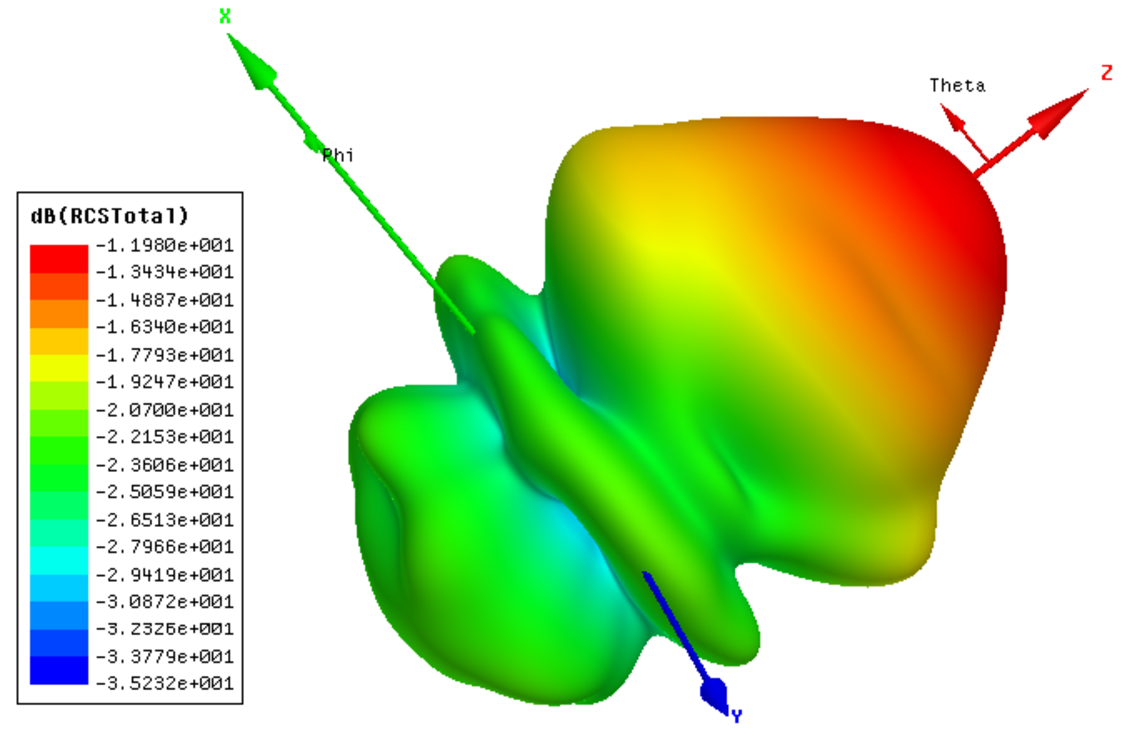
\includegraphics[width=12.4cm]{SphereRCSHFSS}
\caption{Radar cross section of the sphere, computed with HFSS.}
\label{fig:SphereRCSHFSS}
\end{figure}

\begin{figure}[h]
\centering
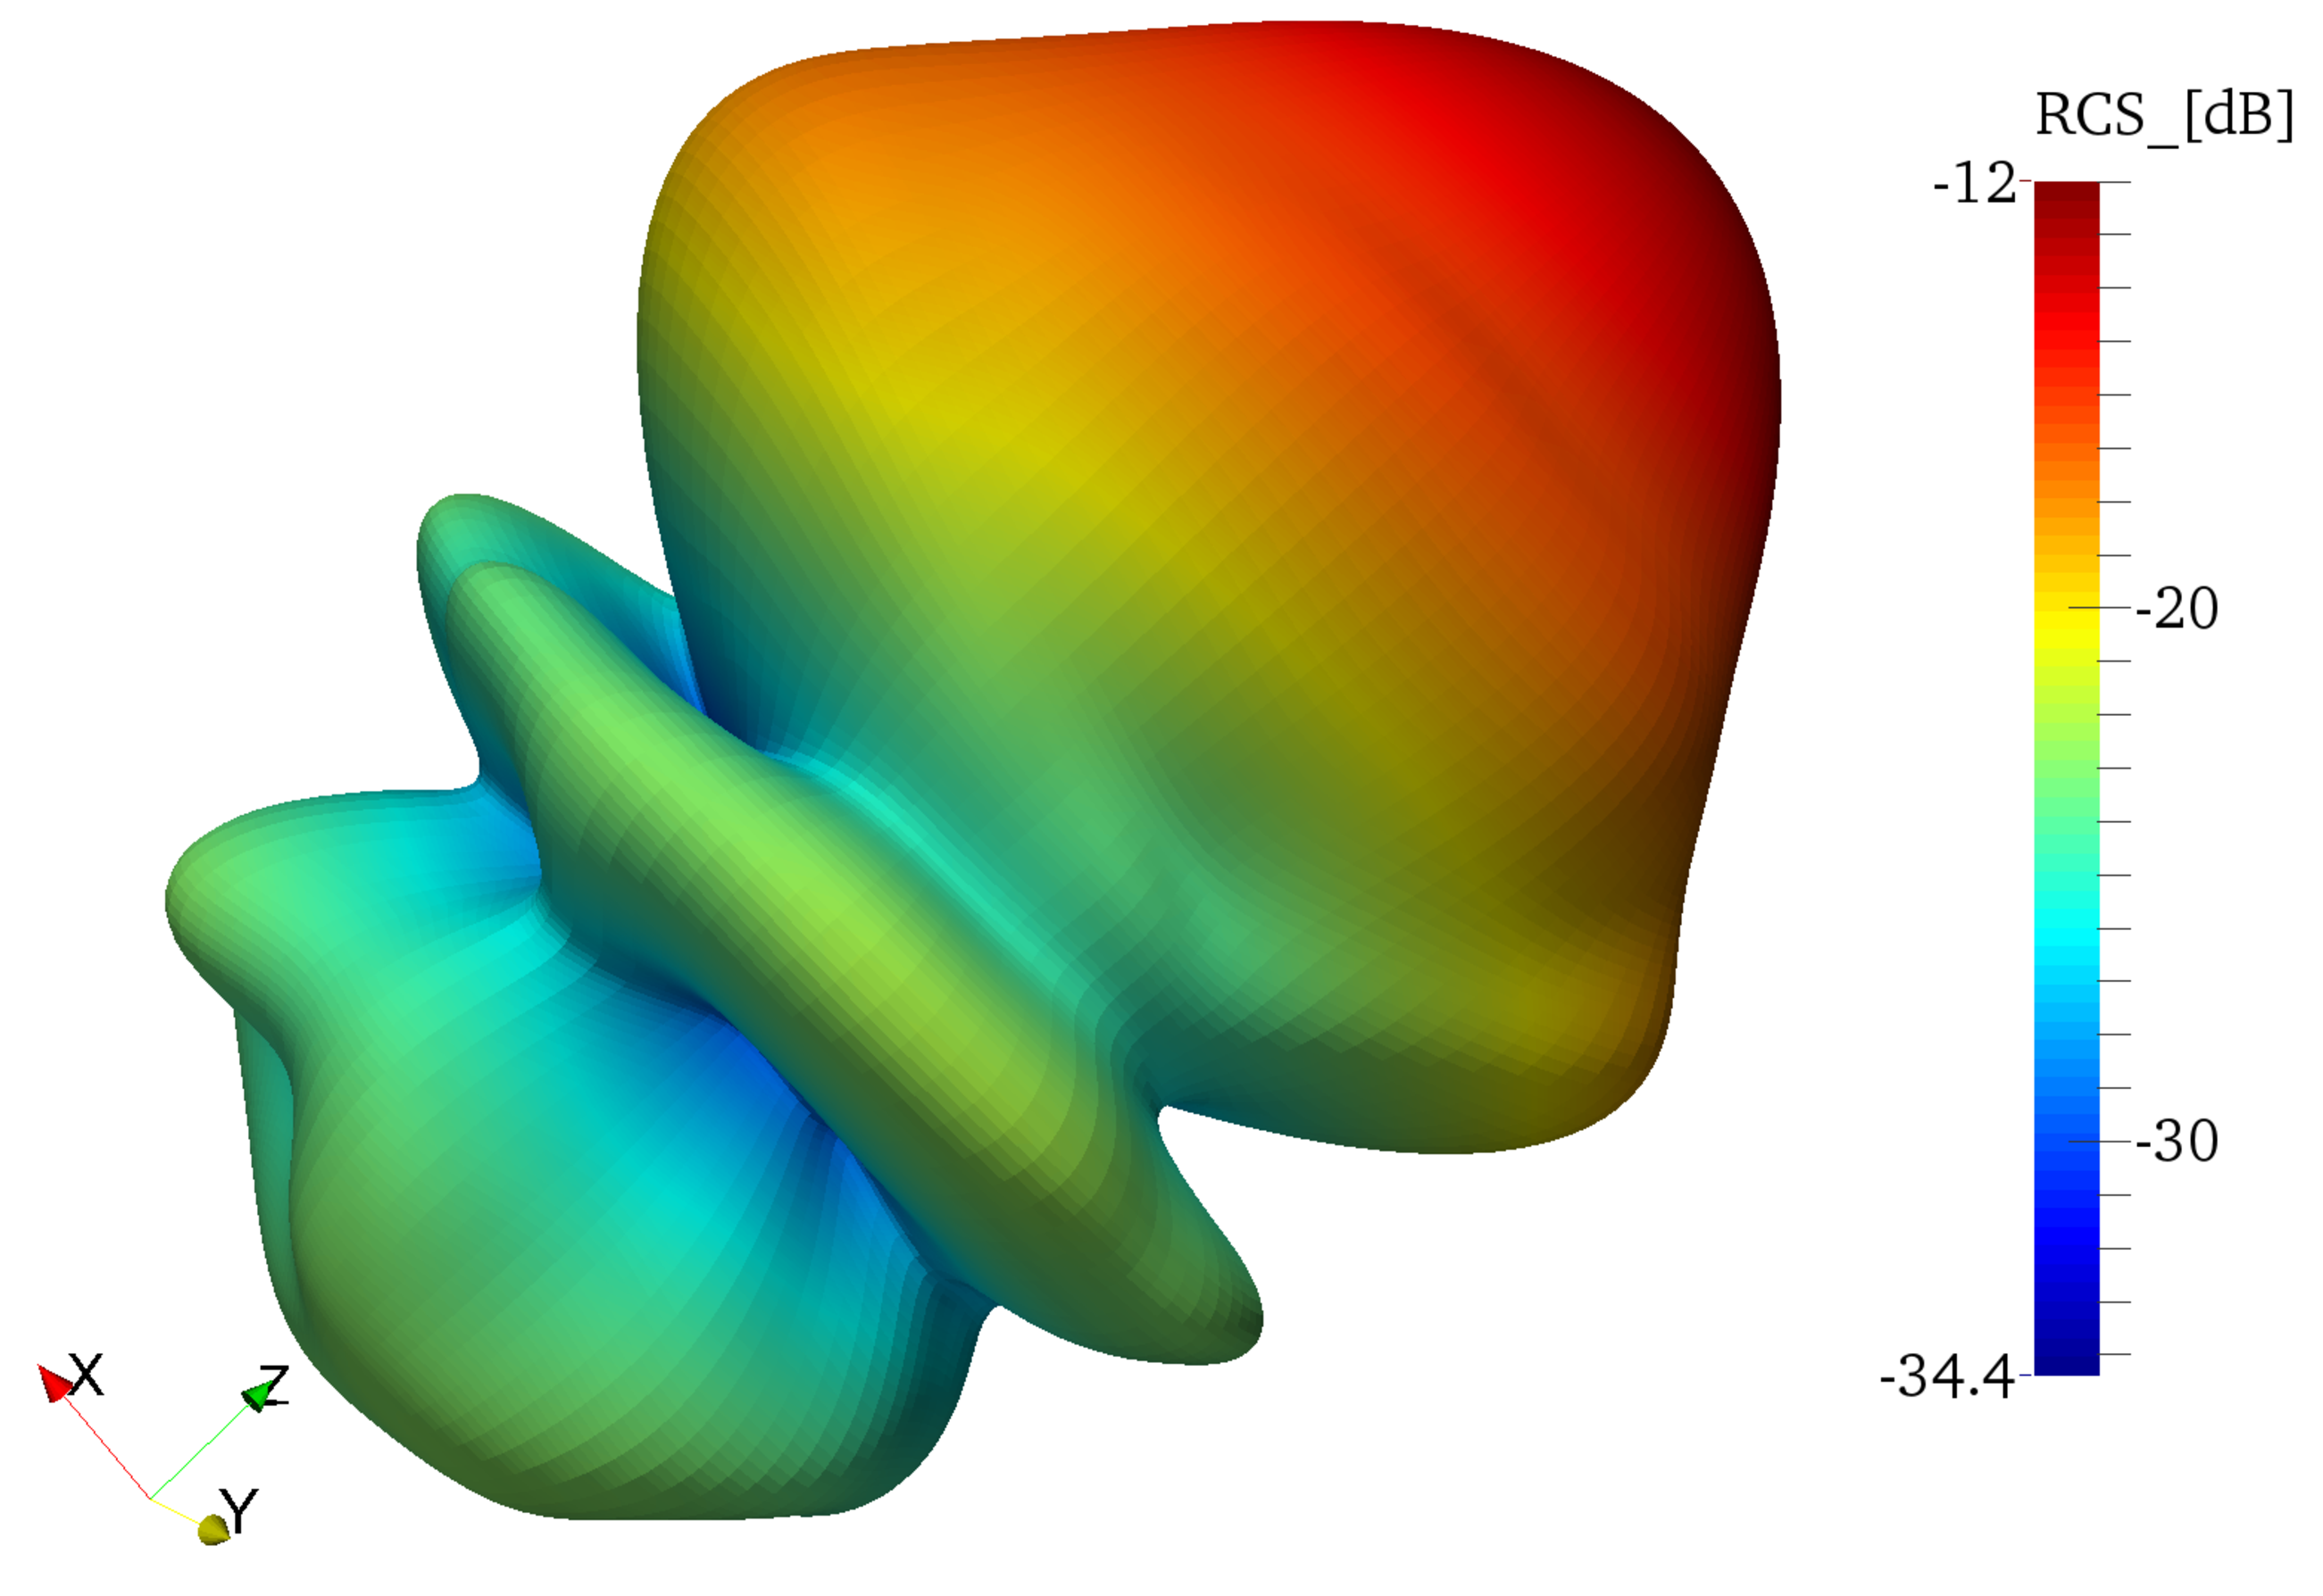
\includegraphics[width=11cm]{SphereRCS}
\caption{Radar cross section of the sphere, computed with FES.}
\label{fig:SphereRCS}
\end{figure}
\clearpage
As said previously, in Paraview it is possible to visualize the electric far field vectors (in the limit of $r\rightarrow \infty$), and hence its polarization. In Fig. \ref{fig:SpherePol}, these vectors are shown and one can see that the fields scattered in $\hat{\mathbf{z}}$-direction remain polarized as the impinging wave, while in other directions the fields might change their polarization.

\begin{figure}[h]
\centering
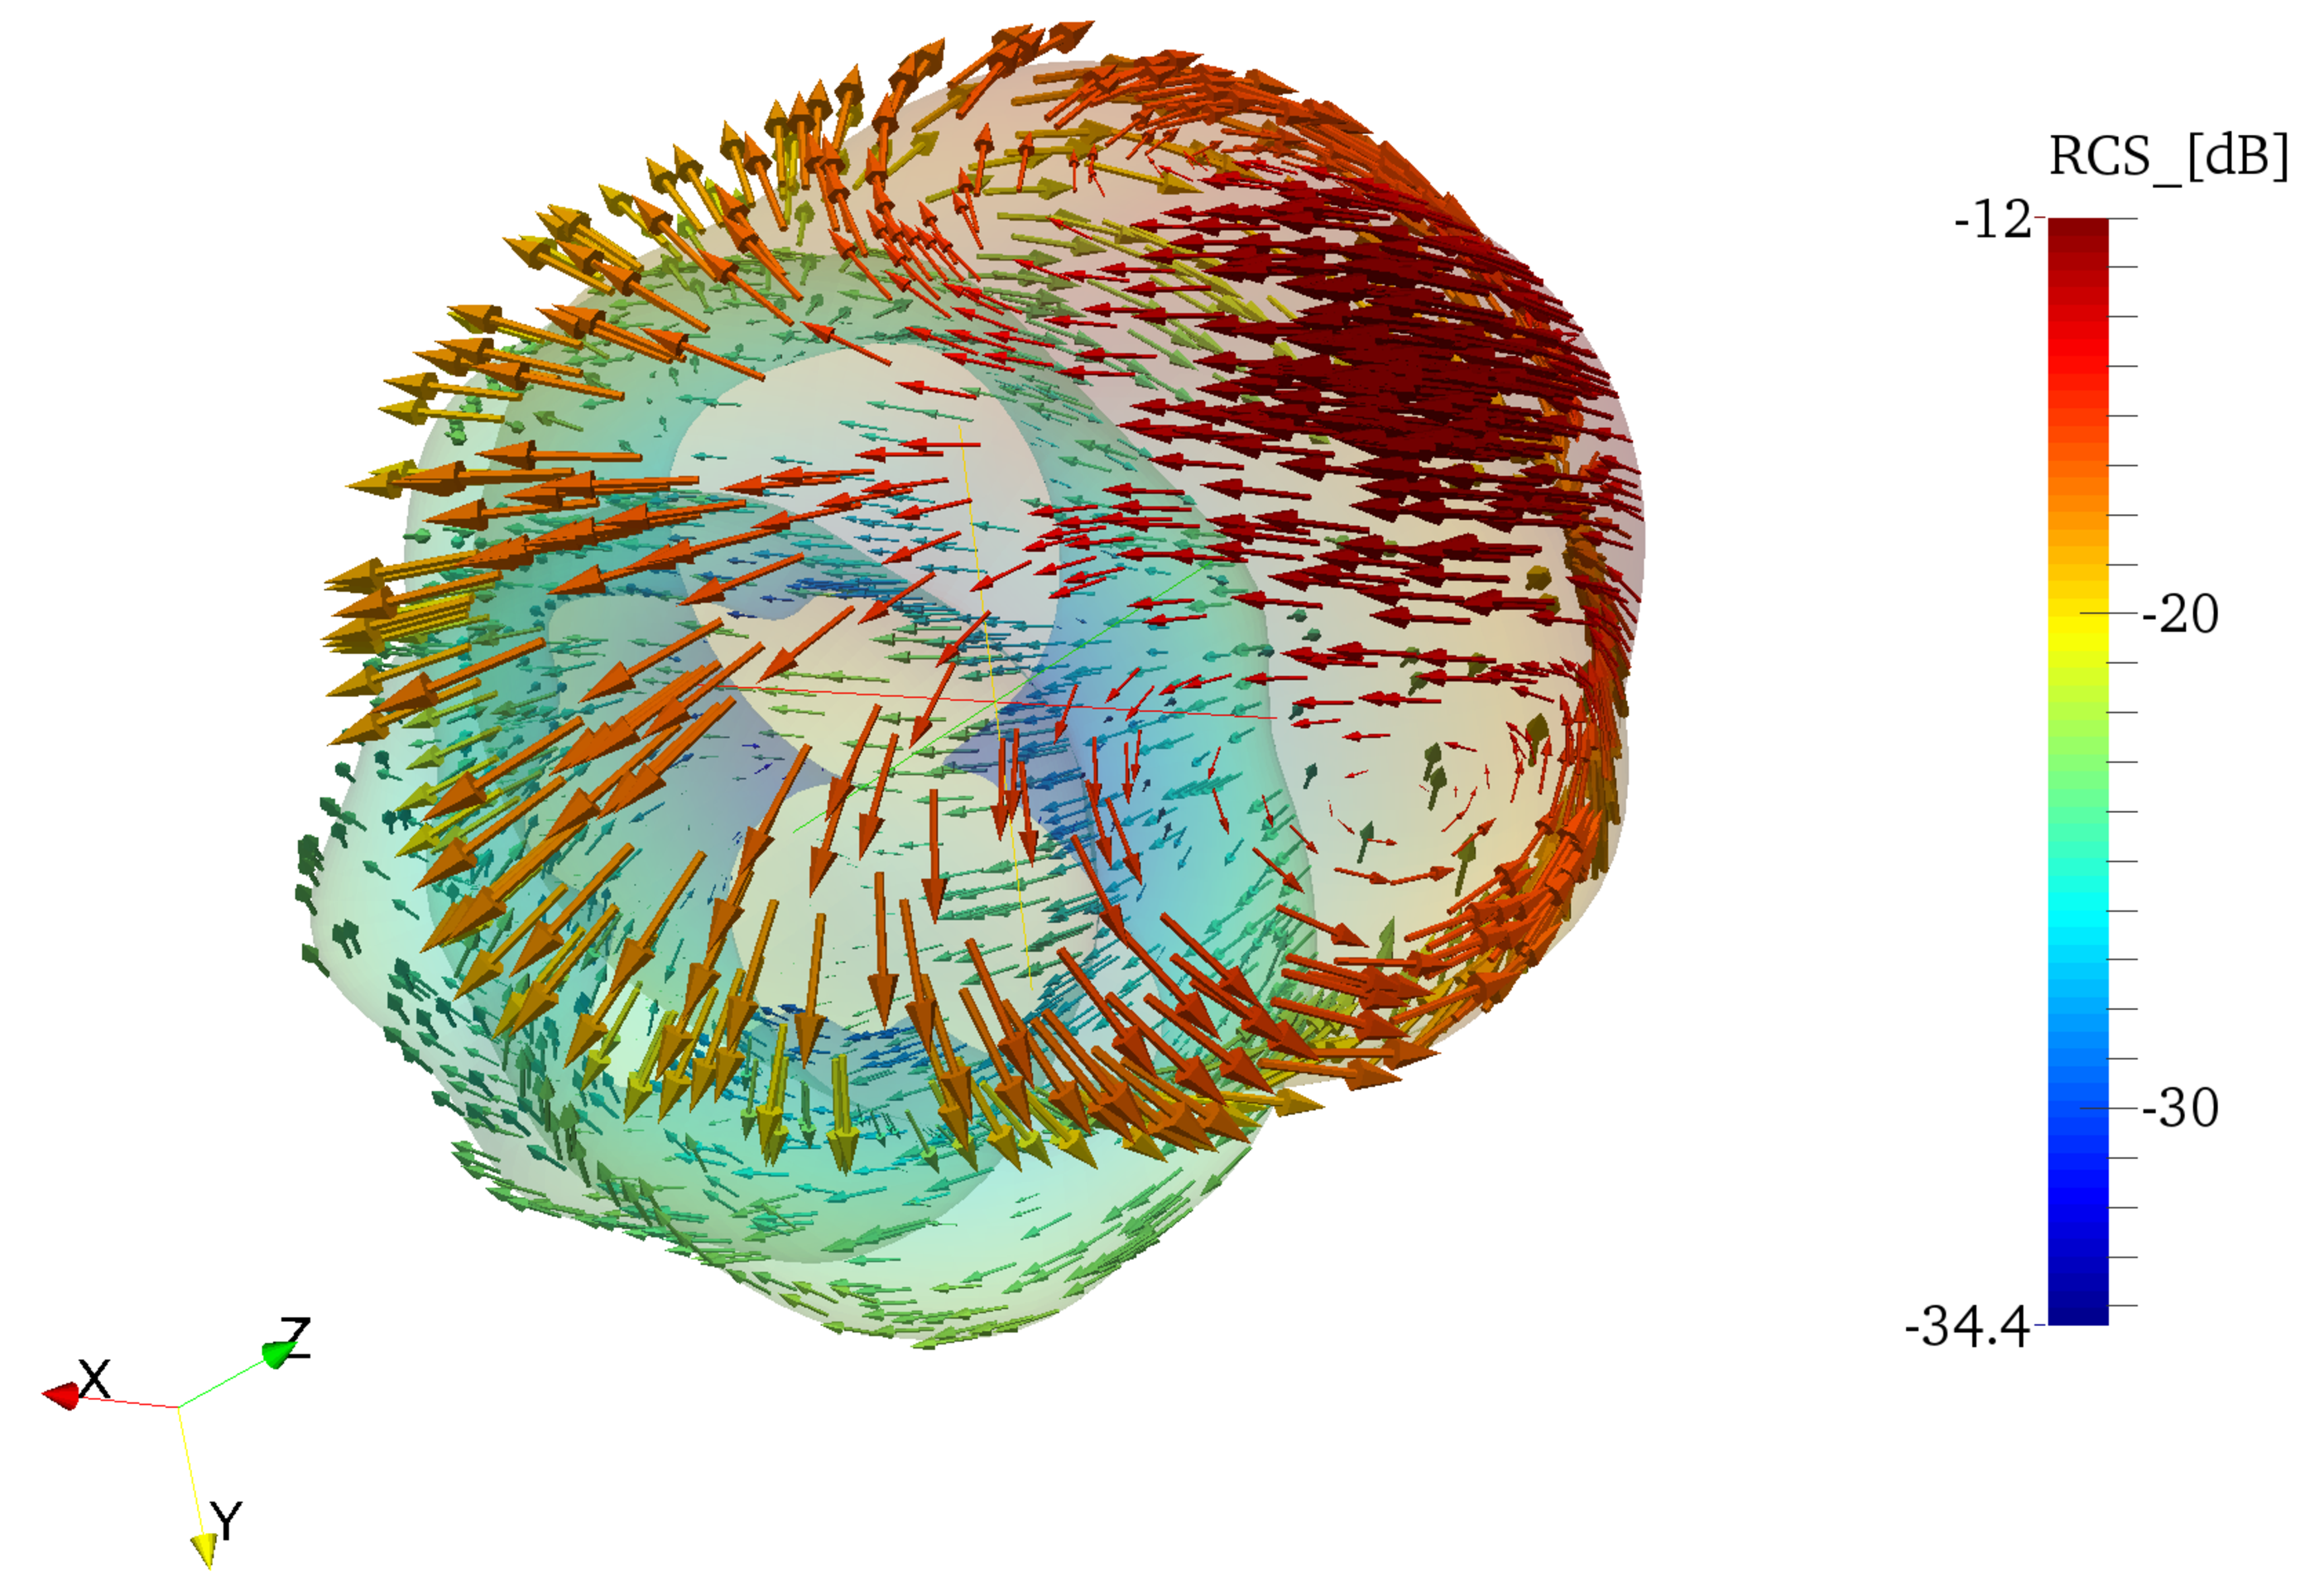
\includegraphics[width=12cm]{SpherePol}
\caption{Polarization of the electric far field visualized with Paraview.}
\label{fig:SpherePol}
\end{figure}